% Single-file version of the paper, generated by paper/scripts/make_single_file.py
% from main.tex, tables/*.tex and references.bib. Do not edit by hand: edit those and rerun.
\documentclass[conference]{IEEEtran}
% ---- begin tables/preamble ----
% Add to the paper's preamble (or % Add to the paper's preamble (or % Add to the paper's preamble (or % Add to the paper's preamble (or \input{tables/preamble} after \documentclass).
\usepackage{booktabs}          % \toprule \midrule \bottomrule
\usepackage[table]{xcolor}     % \cellcolor
\usepackage{graphicx}
\definecolor{bestbg}{RGB}{226,239,218}
% Best corrected model per engine and column (reviewer item #42: "color the best").
\newcommand{\best}[1]{\cellcolor{bestbg}\textbf{#1}}
% Bengali text (example table, review item T4). Needs XeLaTeX and the bundled
% font fonts/NotoSerifBengali-Regular.ttf (Noto, SIL Open Font License).
% Under pdfLaTeX the Bengali text is replaced by a placeholder so the paper
% still compiles.
\usepackage{iftex}
\ifXeTeX
  \usepackage{fontspec}
  % Times, as IEEEtran uses under pdfLaTeX; loaded by file name so it works
  % on Overleaf, TeX Live and Tectonic alike.
  \setmainfont{texgyretermes}[Extension=.otf, UprightFont=*-regular,
    BoldFont=*-bold, ItalicFont=*-italic, BoldItalicFont=*-bolditalic]
  \newfontfamily\bnfont[Script=Bengali, Path=fonts/, Extension=.ttf]{NotoSerifBengali-Regular}
  \newcommand{\bn}[1]{{\bnfont #1}}
\else
  % latexmkrc makes Overleaf use XeLaTeX anyway. If pdfLaTeX still runs, warn
  % (an error made Overleaf report a failed compile) and show a placeholder.
  \PackageWarningNoLine{preamble}{This paper needs XeLaTeX for its Bengali
    examples (Overleaf: Menu > Compiler > XeLaTeX)}
  \newcommand{\bn}[1]{\textcolor{red}{\textbf{[Bengali text missing: compile with XeLaTeX]}}}
\fi
 after \documentclass).
\usepackage{booktabs}          % \toprule \midrule \bottomrule
\usepackage[table]{xcolor}     % \cellcolor
\usepackage{graphicx}
\definecolor{bestbg}{RGB}{226,239,218}
% Best corrected model per engine and column (reviewer item #42: "color the best").
\newcommand{\best}[1]{\cellcolor{bestbg}\textbf{#1}}
% Bengali text (example table, review item T4). Needs XeLaTeX and the bundled
% font fonts/NotoSerifBengali-Regular.ttf (Noto, SIL Open Font License).
% Under pdfLaTeX the Bengali text is replaced by a placeholder so the paper
% still compiles.
\usepackage{iftex}
\ifXeTeX
  \usepackage{fontspec}
  % Times, as IEEEtran uses under pdfLaTeX; loaded by file name so it works
  % on Overleaf, TeX Live and Tectonic alike.
  \setmainfont{texgyretermes}[Extension=.otf, UprightFont=*-regular,
    BoldFont=*-bold, ItalicFont=*-italic, BoldItalicFont=*-bolditalic]
  \newfontfamily\bnfont[Script=Bengali, Path=fonts/, Extension=.ttf]{NotoSerifBengali-Regular}
  \newcommand{\bn}[1]{{\bnfont #1}}
\else
  % latexmkrc makes Overleaf use XeLaTeX anyway. If pdfLaTeX still runs, warn
  % (an error made Overleaf report a failed compile) and show a placeholder.
  \PackageWarningNoLine{preamble}{This paper needs XeLaTeX for its Bengali
    examples (Overleaf: Menu > Compiler > XeLaTeX)}
  \newcommand{\bn}[1]{\textcolor{red}{\textbf{[Bengali text missing: compile with XeLaTeX]}}}
\fi
 after \documentclass).
\usepackage{booktabs}          % \toprule \midrule \bottomrule
\usepackage[table]{xcolor}     % \cellcolor
\usepackage{graphicx}
\definecolor{bestbg}{RGB}{226,239,218}
% Best corrected model per engine and column (reviewer item #42: "color the best").
\newcommand{\best}[1]{\cellcolor{bestbg}\textbf{#1}}
% Bengali text (example table, review item T4). Needs XeLaTeX and the bundled
% font fonts/NotoSerifBengali-Regular.ttf (Noto, SIL Open Font License).
% Under pdfLaTeX the Bengali text is replaced by a placeholder so the paper
% still compiles.
\usepackage{iftex}
\ifXeTeX
  \usepackage{fontspec}
  % Times, as IEEEtran uses under pdfLaTeX; loaded by file name so it works
  % on Overleaf, TeX Live and Tectonic alike.
  \setmainfont{texgyretermes}[Extension=.otf, UprightFont=*-regular,
    BoldFont=*-bold, ItalicFont=*-italic, BoldItalicFont=*-bolditalic]
  \newfontfamily\bnfont[Script=Bengali, Path=fonts/, Extension=.ttf]{NotoSerifBengali-Regular}
  \newcommand{\bn}[1]{{\bnfont #1}}
\else
  % latexmkrc makes Overleaf use XeLaTeX anyway. If pdfLaTeX still runs, warn
  % (an error made Overleaf report a failed compile) and show a placeholder.
  \PackageWarningNoLine{preamble}{This paper needs XeLaTeX for its Bengali
    examples (Overleaf: Menu > Compiler > XeLaTeX)}
  \newcommand{\bn}[1]{\textcolor{red}{\textbf{[Bengali text missing: compile with XeLaTeX]}}}
\fi
 after \documentclass).
\usepackage{booktabs}          % \toprule \midrule \bottomrule
\usepackage[table]{xcolor}     % \cellcolor
\usepackage{graphicx}
\definecolor{bestbg}{RGB}{226,239,218}
% Best corrected model per engine and column (reviewer item #42: "color the best").
\newcommand{\best}[1]{\cellcolor{bestbg}\textbf{#1}}
% Bengali text (example table, review item T4). Needs XeLaTeX and the bundled
% font fonts/NotoSerifBengali-Regular.ttf (Noto, SIL Open Font License).
% Under pdfLaTeX the Bengali text is replaced by a placeholder so the paper
% still compiles.
\usepackage{iftex}
\ifXeTeX
  \usepackage{fontspec}
  % Times, as IEEEtran uses under pdfLaTeX; loaded by file name so it works
  % on Overleaf, TeX Live and Tectonic alike.
  \setmainfont{texgyretermes}[Extension=.otf, UprightFont=*-regular,
    BoldFont=*-bold, ItalicFont=*-italic, BoldItalicFont=*-bolditalic]
  \newfontfamily\bnfont[Script=Bengali, Path=fonts/, Extension=.ttf]{NotoSerifBengali-Regular}
  \newcommand{\bn}[1]{{\bnfont #1}}
\else
  % pdfLaTeX (Overleaf's default) cannot set Bengali. The example table then
  % uses tables/examples_body.pdf, pre-rendered with XeLaTeX; \bn is only a
  % visible fallback for any other Bengali text.
  \PackageWarningNoLine{preamble}{This paper needs XeLaTeX for its Bengali
    examples (Overleaf: Menu > Compiler > XeLaTeX)}
  \newcommand{\bn}[1]{\textcolor{red}{\textbf{[Bengali text missing: compile with XeLaTeX]}}}
\fi
% ---- end tables/preamble ----
\usepackage{amsmath}
\usepackage{cite}
\usepackage{url}

\begin{document}

% Title of the draft Bijon Sir reviewed (D59), with "Historical" added for scope (external review, D63).
\title{Does Zero-Shot Small-Model Post-Correction Help Historical Bengali OCR? A Negative Result Across Eight Models and Two OCR Engines}

\author{\IEEEauthorblockN{Arifur Rahman}
\IEEEauthorblockA{ID: 20234103222\\
Department of Computer Science and Engineering\\
Bangladesh University of Business and Technology\\
Dhaka, Bangladesh\\
arifur.rahman.cs04@gmail.com}}

\maketitle

% =====================================================================
\begin{abstract}
Small open language models are a cheap way to correct optical character recognition (OCR) of historical Bengali books, but we found no study that checks whether they help. We gave the output of two OCR engines for 40 pages from one collection of books printed between 1713 and 1914 to four general-purpose models, four Bengali-pretrained checkpoints and a spell-checker, without examples, and compared the corrected text with human transcriptions. We also tried larger models, a model trained on synthetic errors, and ways to limit the edits. No model on its own significantly lowered the character error rate (CER), and every method changed text that was already correct. Larger Qwen3 models fixed more words than they broke, but their edits to other words added at least as many character errors as the fixes removed. Repetition settings often used against looping made the outputs much worse. Limiting edits to words the engine was unsure of gained about 1\% at best. Until a correction step has been tested against reference transcriptions, the raw OCR should be kept.
\end{abstract}

\begin{IEEEkeywords}
Bengali OCR, post-OCR correction, small language models, zero-shot prompting, historical documents, low-resource NLP, negative results
\end{IEEEkeywords}

% =====================================================================
\section{Introduction}

Archives, libraries and research collections that hold scanned Bengali print need faithful machine-readable text to search their collections, extract information from them, or supply passages to document-based AI systems. OCR turns page images into text but leaves recognition errors, and historical Bengali print is a hard case. Tesseract's character accuracy ranges from 37 to 84 percent across Bengali document types~\cite{rabby2024enhancement}; small stroke differences distinguish many characters, conjunct glyphs combine consonants, and vowel signs can sit before, after, above or below their consonant~\cite{rabby2024enhancement}. Worn type, uneven inking and ornate display lettering add to the difficulty of historical books.

A text-only correction step after OCR is attractive: it needs no change to the engine, it can take the output of any engine, and small open models may suit institutions with limited computing resources~\cite{vershinin2025lightweight}. Such a step is useful only if it repairs recognition errors while preserving text that was already right, including historical spellings, because a fluent rewrite can be a less faithful transcription. Repair and preservation therefore have to be measured separately.

Published results do not settle whether the step helps. Fine-tuned models have improved OCR text~\cite{thomas2024leveraging,beshirov2025bulgarian}, and large models have helped on nearly clean English~\cite{koynov2025opportunities}. Without task-specific training the results are mixed: open models helped English but not Finnish~\cite{kanerva2025nofreelunches}, one of four quantised 7 to 13 billion parameter models improved an English newspaper corpus~\cite{vershinin2025lightweight}, and a 70-billion-parameter model raised error rates once input CER reached about 0.15~\cite{koynov2025opportunities}. Bengali OCR correction has relied on lexicons, morphology and edit distance~\cite{pal2000ocr,ahmed2016improving}, and a commercial model has cleaned OCR text from modern textbooks without a reference-based check of the result~\cite{joy2026bnmmlu}. We found no evaluation of language-model correction on historical Bengali print. Evaluations can also mislead: when greedy decoding loops, the Transformers library offers a repetition penalty and a ban on repeated $n$-grams as remedies, but both also count the prompt~\cite{hf2026logits}, so they penalise a model for copying the very text it should preserve.

We evaluate one correction step applied to the output of two OCR engines on 40 historical Bengali pages, with a control in which the error-free reference is the input. We ask:
\begin{itemize}
\item \textbf{RQ1.} Under the evaluated conditions, do open language models, prompted without task-specific examples, improve historical Bengali OCR relative to keeping the raw output, as measured by character and word error rates?
\item \textbf{RQ2.} How much correctly recognised text do they preserve, and how many recognition errors do they repair?
\item \textbf{RQ3.} How do decoding constraints and the tested safeguards change correction quality?
\end{itemize}
Region-level OCR, synthetic noise, larger and fine-tuned models, and two methods without a language model are extensions that help interpret the answers; Table~\ref{tab:experiments} lists which models and pages each one covers. Our contributions are:
\begin{enumerate}
\item A controlled evaluation of zero-shot post-correction of historical Bengali OCR: eight open models and a dictionary baseline on 40 pages of one collection, read by two engines, with a split frozen before any model was run and character- and word-level outcomes reported separately, extended to region-level OCR, synthetic noise, larger models and a fine-tuned model.
\item A preservation analysis: a clean-text control, counts of correct words broken and wrong words fixed, and an edit-level account of why the word-level repairs of some models do not lower CER.
\item A decoding ablation showing that repetition constraints substantially worsen copying models, on OCR text and on error-free input; in the Transformers library they also act on the prompt, and restricting them to generated tokens removes much, but not all, of the damage. Tests of prompt variants, confidence gating and engine fusion complete it.
\end{enumerate}
The code, page lists, prompts, per-page OCR text and model outputs are released (Section~\ref{sec:repro}).

% =====================================================================
\section{Related Work}

\subsection{Bengali OCR systems}
Bengali OCR research has mostly addressed recognition itself, and document type matters: Rabby et al.\ train separate word-segmentation models for computer-composed, letterpress, typewritten and handwritten material, obtaining character accuracy of 83 to 90 percent compared with Tesseract's 37 to 84 percent~\cite{rabby2024enhancement}. Other work operates at different scales. Safir et al.\ recognise single handwritten words without surrounding context, with CER 0.091 and WER 0.273~\cite{safir2021endtoend}. Chaudhury et al.\ address degraded printed Bangla by separating text from background with a generative adversarial network, then using an encoder-decoder recogniser designed to reduce word error rate~\cite{chaudhury2022deep}. These approaches improve recognition but leave errors on difficult or degraded pages. None supplies a separate correction step for those errors.

\subsection{Post-OCR correction before language models}
Nguyen et al.'s survey describes post-OCR methods developed before large language models and notes the poorer recognition quality of historical material~\cite{nguyen2021survey}. Shared benchmarks came from the ICDAR competitions: about 12 million characters of English and French monographs and periodicals spanning four centuries in 2017~\cite{chiron2017icdar}, then about 22 million characters in ten European languages in 2019, where the best system improved the text by 44\%~\cite{rigaud2019icdar}. Copying is useful in low-resource correction. A model that can copy characters from first-pass OCR reduced error rates by an average of 34\% across three endangered languages~\cite{rijhwani2020ocr}. Bengali approaches have relied on lexical resources. Pal et al.\ parse words into roots and suffixes for lexicon lookup~\cite{pal2000ocr}; Ahmed et al.\ use edit distance and character n-grams with about 541{,}000 dictionary words, lowering error rates by about 3\% on 50 documents~\cite{ahmed2016improving}. Such methods require aligned OCR/reference pairs or language-specific lexicons. We know of no comparable resource for historical Bengali print, hence our interest in models that require no task-specific training.

\subsection{Post-OCR correction with language models}
Table~\ref{tab:literature} summarises the studies closest to ours. It is a selected comparison from targeted searches up to October 2026, including a semantic search of published papers, not a systematic review. Three factors separate success from failure. \emph{Task-specific training} helps most: fine-tuned Llama 2 and BART lowered CER on 19th-century English newspapers~\cite{thomas2024leveraging}, the best HIPE-OCRepair systems combined continued pre-training with fine-tuning and outperformed the zero-shot ones~\cite{ehrmann2026hipeocrepair}, and fine-tuning on synthetic character-level corruption outperformed training on real OCR pairs~\cite{bourne2025scrambled}. Without such training the results are mixed even for large models: fourteen foundation models were ``anything but efficient'' at correcting historical transcripts~\cite{boros2024postcorrection}, instruction-tuned models gave no average CER reduction on German periodicals~\cite{danilova2025german}, and one of four quantised 7 to 13 billion parameter models helped an English newspaper corpus~\cite{vershinin2025lightweight}.

\emph{Input quality} matters too: zero-shot GPT-4o-mini and Llama 3.3 70B lowered newspaper CER at an input CER of 0.07 but raised it at 0.15~\cite{koynov2025opportunities}, a frontier model helped Portuguese survey pages at 0.12~\cite{viana2026reframing}, and over-correction of text that was already accurate recurs, in HIPE-OCRepair and for GPT models on historical English~\cite{zhang2024prosody}.

\emph{Language and register} matter as well: open models improved English but not Finnish~\cite{kanerva2025nofreelunches}, a supervised system improved historical Bulgarian but was specific to its language and engine~\cite{beshirov2025bulgarian}, modern spelling correction suits historical text poorly~\cite{do2025reference}, and multimodal transcription of 18th-century Russian introduced characters from the wrong period~\cite{levchenko2025historical}. Among the studies surveyed here, zero-shot correction helped mainly with large or frontier models and input CER below about 0.15.

\subsection{Bengali language models and tokenisation}
Bengali models differ in whether they can generate text at all. BanglaBERT is an encoder for understanding tasks and cannot rewrite OCR output~\cite{bhattacharjee2022banglabert}; BanglaT5 is a sequence-to-sequence generation model~\cite{bhattacharjee2023banglat5}. The TituLLMs family uses Bengali-pretrained Llama 3.2 models at 1B and 3B, trained on about 37 billion tokens with an extended tokenizer~\cite{nahin2025titullms}. BanglaLlama continues pretraining other Llama models. Its authors report that Bengali and Hindi together account for less than 0.21 percent of Llama 2's pretraining tokens, compared with 89.7 percent for English~\cite{zehady2026banglallama}. Limited exposure is only part of the concern. Mahfuz et al.\ find that inefficient Bengali tokenisation increases computation and reduces generation quality when assessing the need for dedicated Bengali models~\cite{mahfuz2025toolate}. Across languages, Petrov et al.\ show that English-centric tokenizers require several times more tokens for equivalent content; Bengali needs roughly five to ten times the English count, compared with about 1.4 to 1.6 times for multilingual XLM-R and M2M100 tokenizers~\cite{petrov2023tokenizer}. Ahia et al.\ also associate over-segmentation with higher cost and poorer model performance~\cite{ahia2023cost}. General multilingual models therefore face both limited Bengali exposure and inefficient tokenisation. To our knowledge, Bengali-pretrained models have not been evaluated on OCR correction.

\subsection{Correction of Bengali and other Indic text}
The closest Bengali language-model correction study concerns grammar rather than OCR. Instruction-tuning improved its scores by 3 to 7 points over zero-shot use, though humans still did better. Mixing the older literary register with the modern register was among GPT-4o's hardest error categories~\cite{bhattacharyya2025banglagec}. In Hindi speech-recognition correction, fine-tuned models of 0.3 to 0.58 billion parameters outperformed much larger models. Zero-shot GPT-4o-mini increased WER from 28.6 to 31.8 and from 18.0 to 25.1 percent; the authors attribute this to over-correction that grows with model size~\cite{kumar2026postasr}. For Indic OCR, fine-tuned sequence-to-sequence models improved Sanskrit text, the byte-level ByT5 most~\cite{maheshwari2022sanskrit}, and a fine-tuned model given the surrounding sentence improved Hindi, Gujarati and Marathi OCR~\cite{bhandari2026contextual}. Supervised Bengali spelling systems include BSpell, which combines BERT and a convolutional sub-network and outperforms earlier checkers on two Bengali datasets and one Hindi dataset~\cite{rahman2023bspell}, and a transformer detector-purificator-corrector for Bengali and other resource-scarce Indic languages~\cite{bijoy2025transformer}. BnMMLU provides an example of language-model use after Bengali OCR: GPT-3.5 copy-edited EasyOCR output from modern textbooks and exam guides during dataset preparation. The authors report fewer formatting and spelling errors and manually check about 10\% of the items, but give no reference-based error rate for that step~\cite{joy2026bnmmlu}.

\subsection{Research gap}
The Bengali studies cover modern grammar and spelling, lexicon-based OCR correction~\cite{pal2000ocr,ahmed2016improving}, or unmeasured cleaning of modern print; we found no evaluation of language-model correction on historical Bengali print. Among the post-OCR studies in Table~\ref{tab:literature}, none prompts open models below seven billion parameters, reports an input CER above 0.25, applies one correction step across OCR engines, or tests how decoding settings change the result. Our evaluation addresses these gaps in language, scale, engine coverage and evaluation method.

% ---- begin tables/literature ----
% Literature comparison table (reviewer item #10: "Add tables if possible").
% Every cell was checked against the paper itself; see reviewer-feedback/paper-reviews.md.
% Row Zhang et al. (added 2026-10-18) was checked against its abstract (DocEng record). Preprints are not cited (author rule).
% Keys refer to paper/references.bib.
\begin{table*}[t]
\centering
\caption{Language-Model Correction of Recognition Output: Prior Work and This Study}
\label{tab:literature}
\setlength{\tabcolsep}{3.5pt}
\footnotesize
\renewcommand{\arraystretch}{1.15}
\begin{tabular}{>{\raggedright\arraybackslash}p{2.7cm}>{\raggedright\arraybackslash}p{1.25cm}>{\raggedright\arraybackslash}p{1.45cm}>{\raggedright\arraybackslash}p{3.3cm}>{\raggedright\arraybackslash}p{1.6cm}>{\raggedright\arraybackslash}p{1.55cm}>{\raggedright\arraybackslash}p{3.65cm}}
\toprule
Study & Language & Task & Models (size) & Setting & Input error & Did correction help? \\
\midrule
Thomas et al.~\cite{thomas2024leveraging} & English & post-OCR & Llama 2 (7B, 13B); BART & fine-tuned & CER 0.08 & Yes: CER $-$54.5\% (13B) \\
Danilova \& Aangenendt~\cite{danilova2025german} & German & post-OCR & Llama 2 13B, Mistral 7B; BART & fine-tuned & CER 0.02 & No CER gain on average; WER $-$22\% (best) \\
Kanerva et al.~\cite{kanerva2025nofreelunches} & English, Finnish & post-OCR & open models 8B--70B; GPT-4o & zero-shot & CER 0.07 / 0.09 & English: 6 of 7 models; Finnish: only GPT-4o \\
Koynov \& Doan~\cite{koynov2025opportunities} & English, German & post-OCR & GPT-4o-mini; Llama 3.3 70B & zero-shot (+ fine-tuned) & CER 0.07--0.25 & Yes at CER 0.07; worse at CER $\geq$0.15 \\
Vershinin et al.~\cite{vershinin2025lightweight} & English & post-OCR & 7B--13B, 4-bit quantized & zero-shot & CER 0.08 & 1 of 4 models improved CER \\
Beshirov et al.~\cite{beshirov2025bulgarian} & Bulgarian & post-OCR & BERT detector + LSTM corrector & supervised & --- & Yes \\
Ehrmann et al.~\cite{ehrmann2026hipeocrepair} & English, French, German & post-OCR & 8B--24B & zero-shot; fine-tuned & CER 0.004--0.057 & Fine-tuned: yes; zero-shot: mixed (worse than raw OCR on French) \\
Viana~\cite{viana2026reframing} & Portuguese & post-OCR & GPT-5.5 (frontier) & zero-shot & CER 0.12 & Yes: CER $-$60\% \\
Zhang et al.~\cite{zhang2024prosody} & English & post-OCR & GPT-3.5-turbo, GPT-4, GPT-4-turbo & prompted & --- & Yes: CER $-$18.9\% (best, mean); over-corrects good OCR \\
Bhattacharyya \& Bhattacharya~\cite{bhattacharyya2025banglagec} & Bengali & grammar correction & 1.1B--8B; GPT-4o & zero-shot; fine-tuned & clean modern text & Fine-tuned 3--7 points above zero-shot \\
Kumar et al.~\cite{kumar2026postasr} & Hindi & post-ASR & Llama 1B--70B, GPT-4o-mini; mT5, ByT5 (0.3--0.58B) & zero-shot; fine-tuned & WER 0.18--0.29 & Zero-shot: worse; fine-tuned small models: yes \\
\midrule
\textbf{This study} & \textbf{Bengali} & \textbf{post-OCR} & \textbf{0.25B--8B; 32B on 10 pages; SymSpell; engine fusion} & \textbf{zero-shot; one fine-tuned pilot} & \textbf{CER 0.23--0.34} & \textbf{No significant CER reduction by any ungated model; gating $-$0.004 (exploratory), fusion $-$0.003 (descriptive)} \\
\bottomrule
\end{tabular}
\end{table*}
% ---- end tables/literature ----

% =====================================================================
\section{Methodology}

\subsection{Overview}
Each page passes through two OCR engines, then through a correction model in chunks (Fig.~\ref{fig:method}). We score both versions of the text against its manual transcription. Keeping recognition and correction separate lets the same correction step accept output from any engine. All models are used as released, without training or fine-tuning, except in one fine-tuning experiment. The main evaluation covers eight core models and a dictionary baseline. Diagnostic analyses and extensions cover the subsets listed in Table~\ref{tab:experiments}; the extensions are described in Section~\ref{sec:further}.

% ---- begin tables/experiments ----
% Experiment map (editorial review 2026-10-18, sec. 3 and 5; test families added
% after the external review of 2026-10-19, items 6 and 10). Hand-written design
% table: it lists which models, pages and inputs each analysis covers and how it
% is tested, no results. Family sizes checked against the generated table notes.
\begin{table*}[t]
\centering
\caption{Experiment Map: Models, Pages, Inputs and Test Families of Each Analysis}
\label{tab:experiments}
\setlength{\tabcolsep}{3pt}
\footnotesize
\renewcommand{\arraystretch}{1.12}
\begin{tabular}{>{\raggedright\arraybackslash}p{2.8cm}>{\raggedright\arraybackslash}p{4.6cm}>{\raggedright\arraybackslash}p{0.9cm}>{\raggedright\arraybackslash}p{3.2cm}>{\raggedright\arraybackslash}p{3.9cm}>{\raggedright\arraybackslash}p{1.2cm}}
\toprule
Analysis & Correction methods & Pages & Inputs & Tests & Section \\
\midrule
Main evaluation & 8 core models (Gemma-2B-it, Qwen3 1.7B, Phi-4-mini, Llama 3.2 1B, BanglaT5, TituLLMs 1B, 1B Instruct, 3B Instruct) and SymSpell & 40 & Tesseract, EasyOCR, clean text & \textbf{Primary}: 36 (CER, WER), Holm. Exploratory: 18 per secondary measure, Holm; equivalence, unadjusted & \ref{sec:main}, \ref{sec:clean} \\
Decoding ablation & 4 general-purpose core models & 40 & Tesseract, EasyOCR (not Phi-4-mini), clean text & Exploratory: 33, Holm & \ref{sec:decoding} \\
Constraints on generated tokens & 4 general-purpose core models & 40 & Tesseract, clean text & Exploratory: 24 per comparison (vs plain, vs whole sequence), Holm & \ref{sec:decoding} \\
Prompt and chunking variants & 4 general-purpose core models & 40 & Tesseract, EasyOCR & Exploratory: 32, Holm & \ref{sec:variants} \\
Precision and prompt format & TituLLMs 3B Instruct and Phi-4-mini in float32; TituLLMs 1B with a completion prompt (1B and 3B Instruct: Tesseract text); BanglaT5 with its normaliser & 40 & as in the main runs (Phi-4-mini: Tesseract only) & Exploratory, unadjusted (Instruct: Holm over 2) & \ref{sec:precision} \\
Confidence gating & outputs of the main evaluation & 40 & Tesseract, EasyOCR & Exploratory: 54, Holm & \ref{sec:gating} \\
Page-level safeguards & outputs of the main evaluation & 40 & Tesseract, EasyOCR & Exploratory: 18 and 72, Holm & \ref{sec:safeguards} \\
Region-level OCR & 8 core models, SymSpell, Qwen3 4B & 40 & Tesseract and EasyOCR region text & Exploratory: 20 per metric, Holm & \ref{sec:region} \\
Synthetic noise & 4 general-purpose core models & 40 & references at 5 noise levels & Exploratory: 20 per metric, Holm & \ref{sec:noise} \\
Model size & Qwen3 0.6B, 4B, 8B; Gemma~3 1B, 4B; Llama 3.2 3B & 40 & Tesseract, EasyOCR, clean text & Exploratory: 18 per metric, Holm & \ref{sec:scale} \\
Large model & Qwen3 32B (4-bit) & 10 & Tesseract, EasyOCR, clean text & Exploratory: 36 per metric, Holm & \ref{sec:scale} \\
Fine-tuning pilot & ByT5-small fine-tuned on synthetic noise & 40 & Tesseract, EasyOCR, clean text & Exploratory: 3 per metric, Holm & \ref{sec:finetune} \\
No language model & SymSpell variants (2 lexicons, edit distance 1 or 2); engine fusion (2 rules) & 40 & Tesseract, EasyOCR, clean text (fusion: EasyOCR base) & Dictionary: exploratory, 12, Holm. Fusion: descriptive & \ref{sec:classical} \\
Edit-level analysis & Qwen3 1.7B, 4B, 8B; Llama 3.2 3B; fine-tuning pilot; fusion & 40 & Tesseract, EasyOCR & Descriptive & \ref{sec:editlevel} \\
Commentary filter & 8 core models & 40 & Tesseract, EasyOCR & Descriptive & \ref{sec:precision} \\
Gradient-based attribution & 8 core models & 10 chunks & Tesseract, clean text & Descriptive & \ref{sec:attribution} \\
CPU timing & 5 core models (Gemma-2B-it, Qwen3 1.7B, Llama 3.2 1B, BanglaT5, TituLLMs 1B) & 15 & Tesseract and EasyOCR text of an earlier OCR run & None & \ref{sec:computing} \\
\bottomrule
\end{tabular}
\par\smallskip
\begin{minipage}{\linewidth}\footnotesize All analyses use plain greedy decoding and the main prompt unless the analysis varies them. Core: the eight models of the main runs. Tests: two-sided Wilcoxon signed-rank tests with paired-bootstrap intervals; the number is the size of the Holm family, which controls the error only within that family. Only the main evaluation's 36 CER and WER tests are confirmatory; the extensions were added after the main evaluation to test explanations of its result.\end{minipage}
\end{table*}
% ---- end tables/experiments ----

\begin{figure*}[t]
\centering
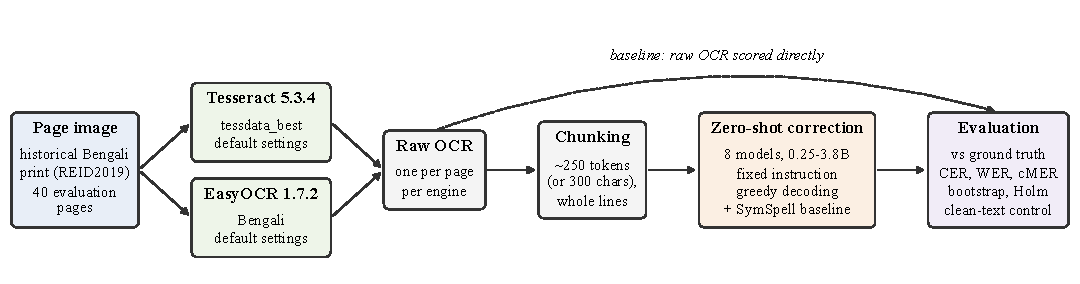
\includegraphics[width=\textwidth]{figures/fig_method.pdf}
\caption{Pipeline of the study. Each page image is read by two OCR engines. The raw text is chunked and corrected zero-shot by one of eight models, or by a dictionary spell-checker, and both raw and corrected text are scored against the ground truth. The dashed arrow marks the uncorrected baseline: raw OCR scored directly.}
\label{fig:method}
\end{figure*}

\subsection{Dataset}
We use the ground-truth transcriptions released with the ICDAR 2019 Competition on Recognition of Early Indian Printed Documents (REID2019)~\cite{clausner2019reid}, produced by the British Library's Two Centuries of Indian Print project with the PRImA Research Lab and Jadavpur University. We use version~2 of the British Library's release, whose XML coordinates were improved~\cite{britishlibrary2019bengaligt}. The source volumes are Bengali books printed between 1713 and 1914. The digitised images are out of copyright and the transcriptions are released under the Public Domain Mark.

The release contains 81 page images with PAGE-XML annotations. Twenty-nine of them (36\%) have text regions marked but no transcribed text, so no error rate can be computed, and they are excluded; 52 pages remain. We drop the two pages with the thinnest transcriptions, measured by the share of text regions that actually contain text, which leaves a pool of 50 pages. The pool is split into 10 development pages and 40 evaluation pages, and the split was frozen in saved page-identifier lists and committed to version control before any correction model was run. The development pages were used to debug the pipeline, as the source of the worked examples in one prompt variant, to estimate the synthetic noise model, as historical training lines for the fine-tuned model, and to choose its checkpoint; they never contribute to a reported evaluation-set estimate. All 40 evaluation pages are scored (Fig.~\ref{fig:dataset}). They come from 37 books, with at most two pages from any one book (Table~\ref{tab:dataset}). The release gives no publication date per book. Each page was labelled by its main content, from its transcription, by a single annotator without a second check: 10 title pages, often in ornate display type, 8 verse pages (including verse followed by a commentary), 13 prose pages, and 9 lists (tables of contents, indexes, tables and dictionary entries); the labels are released with the code. A random sample of 15 of the evaluation pages (seed 403) was also processed on a CPU; it provides the CPU timings and an earlier decoding comparison.

\begin{figure*}[t]
\centering
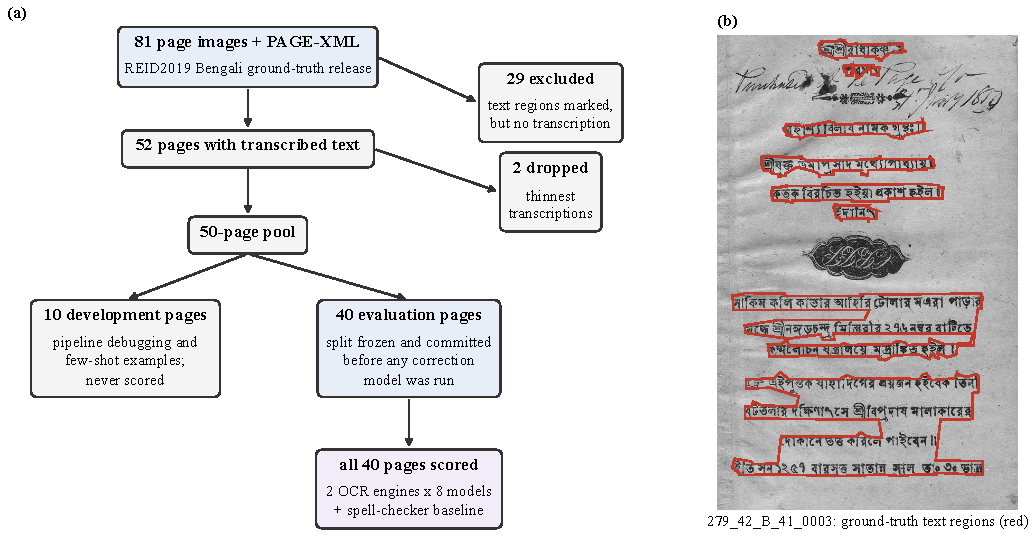
\includegraphics[width=\textwidth]{figures/fig_dataset.pdf}
\caption{Dataset. (a) How the 81 pages of the release become the 40 evaluation pages. (b) A sample evaluation page, with the ground-truth text regions outlined in red.}
\label{fig:dataset}
\end{figure*}

% ---- begin tables/dataset ----
\begin{table}[t]
\centering
\caption{Evaluation Pages}
\label{tab:dataset}
\setlength{\tabcolsep}{4pt}
\footnotesize
\begin{tabular}{ll}
\toprule
Pages & 40 \\
Books & 37 (at most 2 pages per book) \\
Printed & 1713--1914 (no per-book dates) \\
Page types & 10 title, 8 verse, 13 prose, 9 list \\
Reference characters per page & median 577 (range 193--2715) \\
Reference words per page & median 89 \\
Raw Tesseract length / reference & mean 1.03, median 1.00 \\
Raw EasyOCR length / reference & mean 1.02, median 0.99 \\
\bottomrule
\end{tabular}
\par\smallskip
\begin{minipage}{\linewidth}\footnotesize Book: page identifier without its page number. Lengths after Unicode NFC normalisation and whitespace collapsing.\end{minipage}
\end{table}
% ---- end tables/dataset ----

\subsection{Baseline OCR}
\label{sec:ocr}
Two open-source engines produce the noisy text. Tesseract~5.3.4~\cite{smith2007tesseract,tesseract5} runs with its LSTM recogniser and the Bengali \texttt{tessdata\_best} model, and EasyOCR~1.7.2~\cite{jaidedai2024easyocr} with Bengali enabled. Both use their default settings, which for Tesseract means automatic page segmentation (mode~3), and receive the page image as released (colour scans at 400 dpi, about 1{,}800 by 3{,}000 pixels), without preprocessing. Both ran on a free Google Colab CPU runtime on 11 October 2026. Each engine produces one hypothesis per page. Two engines with different error profiles let us test whether correction behaves differently depending on which engine produced its input.

The engines read the whole page, while the ground truth covers only the annotated text regions. Text outside those regions, such as stamps, shelf marks or handwriting (Fig.~\ref{fig:dataset}b), therefore counts as inserted characters. The reference joins the region transcriptions in the order in which they appear in the PAGE-XML file; 30 of the 40 files also declare a reading order, and on 17 pages it differs from the file order. The OCR text keeps each engine's own reading order and is not matched to the reference, so a different order also counts as errors. The mismatch need not cancel in the paired differences, since a model may treat out-of-region text differently from the rest. We therefore repeat the main comparison against a reference in the declared reading order, and with a word-recall measure that ignores word order and extra text (Section~\ref{sec:robustness}), and we repeat the whole evaluation with each region read separately (Section~\ref{sec:further}). OCR output is not stable across installations: an earlier run of Tesseract on the 15-page sample, with an unrecorded Colab build from August 2026, gave different text on all 15 pages (mean CER 0.364 against 0.320), while EasyOCR changed little. Tesseract also drifted within one version. On 12 October, a rerun on Colab with the same version and model file reproduced the main run's text on all 40 pages (this rerun supplied the confidence scores, Section~\ref{sec:gatemethod}). On 17 October, the same setting on Colab and a conda-forge build on Kaggle gave text identical to each other but different from the main run (CER 0.22 between them). The Bengali model file, image decoding and resolution were ruled out; the Leptonica version, image libraries and CPU instruction sets of these runs were not recorded, so the cause cannot be identified. The OCR scripts now record them, with the full version report of Tesseract and a hash of the model file. All reported whole-page results therefore use one stored OCR run, which we release (Section~\ref{sec:repro}); only the CPU timings and the earlier decoding comparison on the 15-page sample use the August text.

\subsection{Correction layer}
\label{sec:correction}
\textbf{Zero-shot.} Each model is used as released, without training on correction examples, and the main prompt contains no worked examples. The decoder models receive an instruction and the OCR text; BanglaT5 receives the text alone, as detailed below. We chose this setting because we know of no large public set of Bengali OCR error pairs for training, and because it avoids the cost of task-specific training.

\textbf{Prompt.} The decoder models receive the same instruction, through each model's chat template:
\begin{quote}
\small\itshape
The following text was produced by OCR on a historical Bengali document and may contain recognition errors. Correct the OCR errors and output only the corrected Bengali text, with no explanation, preamble, or additional commentary.
\end{quote}
The OCR text follows the instruction. BanglaT5 is not instruction-tuned and has no chat template, so it receives the OCR text alone and is run as a text-to-text model. This prompt was fixed in advance and never revised in response to model output.

\textbf{Prompt variants.} For the four general-purpose models we also test three variants, each changing one thing: the same instruction followed by ``Preserve the historical spelling of the original text; if you are not sure whether something is an error, leave it unchanged''; the instruction translated into Bengali; and the instruction with three worked examples. The examples are single lines from three different development pages, chosen by a fixed rule: the first reference line of 30 to 90 characters whose best-matching OCR line has a CER between 0.05 and 0.30 and contains no Latin letters, taking the engines in turn.

\textbf{Chunking.} Following Kanerva et al.~\cite{kanerva2025nofreelunches}, each page is divided into chunks of about 250 tokens of the model's own tokenizer before correction. Chunks are formed by grouping complete lines, so no chunk boundary falls inside a line. Because the tokenizers differ, the resulting chunks range from 168 characters on average for Llama 3.2 1B to 483 for BanglaT5 (Table~\ref{tab:models}). As a model-independent alternative for the four general-purpose models, we also group lines into chunks of at most 300 characters, which every model then receives identically; a single longer line would form its own chunk, but none occurred on our pages.

\textbf{Decoding.} We use greedy decoding, without token sampling. The maximum number of new tokens is $\min(512,\max(64,1.5n))$, where $n$ is the token length of the input chunk, and an output that reaches this limit is counted as truncated. No other constraint is applied in the main condition. A repetition penalty and a ban on repeated $n$-grams are the library's remedies when greedy decoding loops. Both are off unless set (the library's neutral values are a penalty of 1.0 and no ban); a user who meets looping output, as we did on some development pages, may add them. We evaluate them, alone and together, as a decoding ablation (penalty 1.3; repeated four-grams banned; both together are \emph{guarded} decoding; Section~\ref{sec:decoding}). In the Transformers library~\cite{wolf2020transformers}, \texttt{generate} applies \texttt{RepetitionPenaltyLogitsProcessor} and \texttt{NoRepeatNGramLogitsProcessor} to the whole token sequence, which for a decoder-only model includes the prompt and so the OCR text being corrected~\cite{hf2026logits}. In version~5.19.0, which the runs used, the penalty can exclude the prompt only if its processor is constructed by hand, and the $n$-gram ban has no such option. A one-step test with Qwen3 0.6B on that version confirms both: the penalty changed the scores of all 42 distinct token ids of a correction prompt and of no other id, and the ban blocked the token that would repeat a four-token run of the prompt. The constraints then penalise every token the model copies and forbid it to reproduce any four-token run of its input. A follow-up run restricts each constraint to the generated tokens, the penalty through \texttt{prompt\_ignore\_length} and the ban through a processor that sees only the output, for the four general-purpose models on Tesseract and clean text. Since correction is mostly copying, plain greedy decoding is the main condition; decoding settings that suit one generation task need not suit another~\cite{wiher2022decoding}.

\subsection{Choice of models}
We evaluate eight core models of 0.25 to 3.84 billion parameters (Table~\ref{tab:models}). We call a model \emph{small} if it has at most about four billion parameters, so that it can run on a CPU; the larger models of Section~\ref{sec:further} are scale extensions. Parameter counts are computed from each checkpoint's configuration, with tied input and output embeddings counted once.
\begin{itemize}
\item \emph{General-purpose models.} Gemma-2B-it~\cite{gemma2024card} (Gemma~1, 2.51B parameters), Qwen3 1.7B~\cite{qwen2025card}, Phi-4-mini~\cite{phi4mini2025card} and Llama 3.2 1B~\cite{meta2024llama32} are open instruction-tuned multilingual models; Qwen3 and Phi-4-mini were released in 2025. Bengali is a very small share of the pretraining data of general models~\cite{zehady2026banglallama}. Qwen3 can produce a reasoning trace before its answer; we disable this through its chat template, so it answers directly.
\item \emph{Bengali-pretrained checkpoints.} TituLLMs 1B~\cite{nahin2025titullms} (checkpoint v1.1) is Llama 3.2 1B continually pretrained on Bengali text. It is a base model without instruction tuning and keeps the Llama vocabulary; the template shipped with its tokenizer only concatenates the messages, so it received our instruction and the OCR text as plain text to continue, with no cue for where a corrected version should begin. As a check, we also gave it a completion prompt without template, which states that the corrected text follows the OCR text and ends with ``Corrected text:'' (Section~\ref{sec:precision}). We also evaluate the instruction-tuned TituLLMs checkpoints at 1B and 3B parameters (v2.0 Instruct), which use an extended vocabulary of 170{,}497 tokens; their model cards give no prompt format, and their shipped template wraps the prompt in an Alpaca-style instruction and response frame, which we used; as a check, they also received the completion prompt on Tesseract text. BanglaT5~\cite{bhattacharjee2023banglat5} (about 248M parameters) is a sequence-to-sequence model pretrained only to restore corrupted text spans and released without task fine-tuning. Without a task prefix it acts as a denoiser rather than a corrector, so we report it as a control. Its model card also asks for inputs passed through the authors' text normaliser, which the main runs did not apply; a rerun with it is reported in Section~\ref{sec:precision}.
\end{itemize}
These results therefore describe checkpoint-and-prompt configurations, not a ranking of model families, and say nothing about Bengali pretraining in general; we treat the Bengali-pretrained checkpoints as diagnostic cases. BanglaBERT~\cite{bhattacharjee2022banglabert} was not considered because it is an encoder and cannot generate corrected text. All models are loaded with the Transformers library~\cite{wolf2020transformers}. Section~\ref{sec:further} adds newer and larger general-purpose models, up to 32 billion parameters, and one fine-tuned model.

% ---- begin tables/models ----
\begin{table}[t]
\centering
\caption{Models and Configuration}
\label{tab:models}
\setlength{\tabcolsep}{2.5pt}
\footnotesize
\begin{tabular}{>{\raggedright\arraybackslash}p{1.85cm}>{\raggedright\arraybackslash\scriptsize}p{2.75cm}cccc}
\toprule
Model & Checkpoint@revision & \shortstack{Params\\(B)} & \shortstack{GPU\\prec.} & Input & \shortstack{Chars/\\chunk} \\
\midrule
\multicolumn{6}{l}{\textit{General-purpose, instruction-tuned}} \\
Gemma-2B-it & \texttt{google/\allowbreak gemma-\allowbreak 2b-\allowbreak it@\allowbreak 9698841} & 2.51 & fp32 & template & 312 \\
Qwen3 1.7B & \texttt{Qwen/\allowbreak Qwen3-\allowbreak 1.7B@\allowbreak 70d244c} & 1.72 & fp32 & template & 190 \\
Phi-4-mini & \texttt{microsoft/\allowbreak Phi-\allowbreak 4-\allowbreak mini-\allowbreak instruct@\allowbreak cfbefac} & 3.84 & fp16 & template & 389 \\
Llama 3.2 1B & \texttt{meta-\allowbreak llama/\allowbreak Llama-\allowbreak 3.2-\allowbreak 1B-\allowbreak Instruct@\allowbreak 9213176} & 1.24 & fp32 & template & 168 \\
\multicolumn{6}{l}{\textit{Bengali-pretrained (diagnostic)}} \\
BanglaT5 & \texttt{csebuetnlp/\allowbreak banglat5@\allowbreak 76b135c} & 0.25 & fp32 & text & 483 \\
TituLLMs 1B & \texttt{hishab/\allowbreak titulm-\allowbreak llama-\allowbreak 3.2-\allowbreak 1b-\allowbreak v1.1@\allowbreak 521da71} & 1.24 & fp32 & template & 168 \\
TituLLMs 1B Instruct & \texttt{hishab/\allowbreak titulm-\allowbreak llama-\allowbreak 3.2-\allowbreak 1b-\allowbreak v2.0-\allowbreak Instruct-\allowbreak v1.0@\allowbreak 039dbd2} & 1.32 & fp32 & template & 422 \\
TituLLMs 3B Instruct & \texttt{hishab/\allowbreak titulm-\allowbreak llama-\allowbreak 3.2-\allowbreak 3b-\allowbreak v2.0-\allowbreak Instruct-\allowbreak v1.0@\allowbreak 6a96004} & 3.34 & fp16 & template & 422 \\
\bottomrule
\end{tabular}
\par\smallskip
\begin{minipage}{\linewidth}\footnotesize Checkpoint: Hugging Face model and revision. Parameters from each checkpoint's configuration, tied embeddings counted once. GPU prec.: precision on the T4 (fp16 for the two models whose fp32 weights exceed its memory). Input: the prompt through the chat template shipped with the checkpoint, or the OCR text alone. Chars/chunk: mean characters per chunk of about 250 tokens on raw Tesseract text. Decoding for all models: greedy, at most $\min(512,\max(64,1.5n))$ new tokens, no repetition penalty or n-gram ban.\end{minipage}
\end{table}
% ---- end tables/models ----

% ---- begin tables/cost ----
\begin{table}[t]
\centering
\caption{Tokenisation and Computational Cost}
\label{tab:cost}
\setlength{\tabcolsep}{2pt}
\footnotesize
\begin{tabular}{lccccc}
\toprule
Model & \shortstack{Tokens/\\char} & \shortstack{Tokens/\\word} & \shortstack{GPU weights\\(GB)} & \shortstack{CPU\\min/page} & \shortstack{GPU\\min/page} \\
\midrule
Gemma-2B-it & 0.60 & 3.9 & 10.0 & 10.4 & 0.38 \\
Qwen3 1.7B & 1.08 & 7.1 & 6.9 & 14.3 & 0.58 \\
Phi-4-mini & 0.45 & 3.0 & 7.7 & --- & 0.31 \\
Llama 3.2 1B & 1.22 & 8.0 & 5.0 & 9.5 & 0.37 \\
BanglaT5 & 0.29 & 1.9 & 1.0 & 2.2 & 0.05 \\
TituLLMs 1B & 1.22 & 8.0 & 5.0 & 12.5 & 0.59 \\
TituLLMs 1B Instruct & 0.38 & 2.5 & 5.3 & --- & 2.44 \\
TituLLMs 3B Instruct & 0.38 & 2.5 & 6.7 & --- & 0.32 \\
\bottomrule
\end{tabular}
\par\smallskip
\begin{minipage}{\linewidth}\footnotesize Tokens/char and tokens/word: each tokenizer on the 40 reference texts. GPU weights: parameters $\times$ 4 bytes in fp32 or 2 in fp16; peak memory during generation was not recorded. GPU: NVIDIA T4, plain decoding, the 40 pages of the main setting. CPU: free Colab CPU runtime in bfloat16, plain decoding, on the 15-page sample with its August 2026 OCR, a different input from the main setting (---: not run on CPU). Times are per page and engine.\end{minipage}
\end{table}
% ---- end tables/cost ----

\subsection{Classical baseline}
To test whether the outcome is specific to language models, we also correct the OCR with a dictionary spell-checker. SymSpell~\cite{garbe2025symspell} replaces every Bengali word that is not in its lexicon with the lexicon word at the smallest edit distance, breaking ties by frequency, if one exists within an edit distance of 2; known words, punctuation, digits and Latin text are left unchanged. The lexicon is the 50{,}000 most frequent words of the Bengali OpenSubtitles corpus~\cite{dave2018frequencywords}, of which 44{,}335 entries consist only of Bengali letters and signs. Its settings are the library defaults, fixed in advance. Because subtitles are modern and colloquial, we also test a lexicon of the 100{,}000 most frequent words of Bengali Wikipedia~\cite{wikimedia2023wikipedia} (143{,}069 articles), and an edit distance of 1 with each lexicon.

\subsection{Computing setting}
\label{sec:computing}
The motivating setting is CPU-only use by institutions that process Bengali documents without GPU infrastructure, so the eight core models were chosen small enough to run on a CPU; the larger models of the extensions need a GPU. All reported scores, however, come from GPU runs. Table~\ref{tab:cost} reports the CPU time per page for the five core models that were run on a free Google Colab CPU runtime in bfloat16, with plain decoding, on the 15-page sample and its August OCR text, so these times describe a different input from the main runs. The reported runs use free NVIDIA T4 GPUs on Kaggle, in float32, or in float16 for the two core models above 3B parameters, which do not fit the GPU's 15~GB in float32; float32 reruns of these two on two Kaggle T4 GPUs (Section~\ref{sec:precision}) and a CPU-against-GPU comparison (appendix) gave practically the same scores. No paid service is used at any stage.

\subsection{Metrics}
Before scoring, reference and hypothesis are normalised to Unicode NFC and runs of whitespace are collapsed, because Bengali conjuncts and vowel signs can be encoded as different code-point sequences that look identical. Zero-width joiners and non-joiners are kept, and the danda counts as an ordinary character. The character error rate is $\mathrm{CER}=(S+D+I)/N$, where $S$, $D$ and $I$ are the numbers of substituted, deleted and inserted characters in the alignment of the hypothesis with the reference and $N$ is the number of reference characters; the word error rate (WER) is the same quantity over words. Both are computed with jiwer~\cite{vaessen2022jiwer} for each page and averaged over pages, so every page counts equally regardless of its length; the pooled CER divides the total number of character errors by the total reference length. CER counts code points, so an error in one sign of a conjunct counts once although the reader sees the whole cluster as wrong; the grapheme-cluster CER is computed over extended grapheme clusters, which keep a conjunct and its vowel signs together. CER and WER are unbounded, since an output with many insertions can score above 1. We therefore also report the character and word match error rates, $\mathrm{cMER}=(S+D+I)/(H+S+D+I)$ and its word-level counterpart wMER, where $H$ is the number of matched units; both are bounded in $[0,1]$~\cite{ehrmann2026hipeocrepair}. Three further normalisations test the scoring choices: mapping ASCII digits to Bengali digits, removing zero-width joiners and non-joiners, and writing khanda-ta as the single code point U+09CE. CER and WER are the primary measures; CER always means the code-point CER unless named otherwise. The grapheme-cluster CER, cMER, wMER, pooled CER, a CER with all spaces removed and the reference-word recall of Section~\ref{sec:analyses} are secondary checks. They are not interchangeable: recall ignores word order and extra text, so it cannot penalise insertions or a wrong order, and it does not reward a repair that leaves a word wrong.

\subsection{Statistics}
For each engine and correction method, the unit of analysis is the per-page difference between the corrected and the uncorrected error rate. We report the mean difference with a 95\% percentile interval from a paired bootstrap of the 40 pages (10{,}000 resamples, seed 403), and the number of pages whose error rate fell or rose. We also run a two-sided Wilcoxon signed-rank test~\cite{wilcoxon1945} on the same differences. Pages whose difference is exactly zero, which are common when a method leaves the OCR unchanged, are dropped before ranking, the default of the test, so we report how many pages remain. The primary family is the 36 CER and WER tests (nine methods, two engines, two metrics), adjusted with the Holm procedure~\cite{holm1979}, which follows the reporting of Viana~\cite{viana2026reframing}. Every other test in this paper is exploratory: each table that reports one names its own Holm family, and Holm controls the error only within a family. Because pages from the same book are not independent, we repeat the bootstrap resampling whole books instead of pages. The four general-purpose models stay close to the raw OCR, but no detectable change is not the same as no change. We therefore test equivalence with two one-sided paired $t$-tests (TOST) against margins of $\pm0.01$ and $\pm0.02$ CER. The margins are about 3\% and 6\% of the raw CER, a change a user comparing transcriptions would hardly notice, and small next to the changes of the other methods. Because per-page differences can be heavy-tailed, we also check whether the 90\% paired-bootstrap interval lies within the margin; it gives the same decisions. Table~\ref{tab:experiments} lists every test family with its size and role: the primary family above, exploratory families with Holm correction within each, and descriptive analyses without tests.

The evaluation split was frozen before any model ran, and development pages never contribute to a reported evaluation-set estimate. We used this one fixed evaluation set and did not perform cross-validation. Greedy decoding removes sampling randomness, so the zero-shot runs were not repeated with different seeds; it does not guarantee identical outputs across devices or software builds (appendix). The fine-tuning pilot was trained once, with one seed (403).

\subsection{Analyses}
\label{sec:analyses}
\textbf{Sensitivity to the reference.} Two checks address the mismatch between whole-page OCR and region-level ground truth. First, we rebuild each reference with its regions in the reading order declared in the PAGE-XML file, where there is one (regions it does not list follow in file order), and repeat the paired comparison of CER. Second, we compute reference-word recall: the share of reference word tokens that also occur in the output, counted as a multiset. It ignores word order and does not penalise extra words, so neither a different reading order nor OCR text from outside the annotated regions lowers it; it does not reward repairs that leave a word wrong.

\textbf{Clean-text control.} To separate over-correction from the difficulty of noisy input, each model also receives the reference text itself in place of the OCR, with the same prompt and decoding. Any change it makes can then only be damage. The control is a diagnostic stress test of preservation under the tested prompt configuration; it does not estimate the quality of corrected OCR, and it does not rank the models in general.

\textbf{Word-level and edit analysis.} We align the ground-truth words with the raw OCR and with the corrected output. A ground-truth word that the raw OCR matched exactly and the output does not is a \emph{broken} word; a word the raw OCR missed and the output matches is a \emph{fixed} word~\cite{kumar2026postasr}. The \emph{change ratio} is the CER of the output measured against the raw OCR, divided by the CER of the raw OCR against the ground truth~\cite{koynov2025opportunities}; a ratio above 1 means the model changed more than there was to repair. \emph{Invented runs} are runs of at least six characters that the output contains and the raw OCR does not~\cite{koynov2025opportunities}. To see why repaired words need not lower CER, we assign every character error of the alignment with the reference to a reference word (an insertion to the word it follows) and split the change in character errors between fixed, broken and still-wrong words and the spaces between words. Each error is also labelled by the Bengali character class involved (consonant, vowel sign, virama, other sign, digit, punctuation or space). Output length, script shares, word retention, edit operations, character classes, page types and truncation are reported in the appendix.

\textbf{Commentary filter.} As a check on prompt fit, a generous filter drops every output line of which fewer than 30\% of the character trigrams occur in the page's OCR input. It removes preambles and descriptions of the text, but also invented lines, so its scores bound what any such filter could achieve; it is not one of the evaluated methods.

\textbf{Attribution.} To see which part of its input each output token is sensitive to, we adapt Grad-CAM~\cite{selvaraju2017gradcam} to token positions: the score is the logit of each generated token, and the map runs over the token positions of a layer's hidden states. We compute the literal version, which averages the gradient over positions, and an element-wise version, which multiplies gradient and hidden state at each position before summing over the hidden dimensions, at one-half and three-quarter depth, leaving out the first token, special tokens and the predicting position. For each generated token we record the share of the map on the OCR text, the rest of the prompt and the model's own earlier output, and, for a copied token, whether the map peaks within one position of its source. We scored up to 24 generated tokens in one chunk from each of 10 pages (seed 403), on Tesseract and clean text, for the eight core models.

\textbf{Output filter not applied.} Kanerva et al.\ strip leading and trailing text that does not align with the input, such as explanatory preambles~\cite{kanerva2025nofreelunches}. We did not apply this step, so all main scores use unfiltered model output and any preamble or commentary counts as error; the commentary filter above shows how much this matters.

\subsection{Safeguards and confidence gating}
\label{sec:gatemethod}
\textbf{Page-level safeguards.} As post-hoc checks, we replace a model's output by the raw OCR whenever its length falls outside 0.35 to 2.8 times the input length; these thresholds are taken from a zero-shot system in the HIPE-OCRepair task~\cite{ehrmann2026hipeocrepair} and are not tuned on our pages. A second rule, an edit-distance cap, keeps the output only if its CER measured against the raw OCR is at most $\tau$, for $\tau \in \{0.05, 0.1, 0.2, 0.3\}$, a grid fixed in advance. Each safeguarded result is compared with the raw OCR by the same paired bootstrap and Wilcoxon test, with Holm correction over the 18 length-rule tests and, separately, the 72 edit-cap tests.

\textbf{Confidence gating.} Both engines report how confident they are: Tesseract per word (0 to 100) and EasyOCR per detected text box (0 to 1), which every word in the box inherits. We re-ran both engines with the same versions on Colab on 12 October 2026, one day after the main run and before the drift (Section~\ref{sec:ocr}), to obtain these values; the re-run reproduced the stored OCR text on all 40 Tesseract pages and 37 EasyOCR pages, and confidences are mapped onto the stored words by word alignment. On the three EasyOCR pages that were not reproduced, as elsewhere, a stored word without a counterpart in the re-run counts as confident, so the gate never lets a model change it. The existing model outputs are then gated: after aligning the OCR words with the output words, an edit that replaces or deletes OCR words is kept only if every OCR word it touches has a confidence below a threshold, and an inserted word only if a neighbouring OCR word does; all other words stay as the OCR read them. The model therefore still corrects whole chunks with their context, but may change only what the engine was unsure of. The thresholds are fixed in advance: 50, 70 and 90 for Tesseract and 0.5, 0.7 and 0.9 for EasyOCR.

\subsection{Further experiments}
\label{sec:further}
Five further experiments test explanations of the main result: noisy or mismatched input, model size, the lack of training, and the use of a language model at all. Unless stated otherwise they use plain greedy decoding, the main prompt and the main chunking, and each forms its own exploratory Holm family.

\textbf{Region-level OCR.} Each PAGE-XML text region is cropped from the page image (its bounding box plus 8 pixels) and read on its own, Tesseract with page segmentation mode~6, which suits a single block of text. The crop settings were chosen in a comparison on 8 of the evaluation pages with a different Tesseract version (5.5.3), before any model saw region text. These pages therefore influenced the choice, and the region-level OCR scores are not fully independent of it; each correction is still compared with the raw OCR of the same regions. The 576 regions with text are joined in reading order and scored against the reference regions in the same order, so out-of-region text and reading-order differences no longer count as errors. Because of the Tesseract drift (Section~\ref{sec:ocr}), whole pages were read again in the same run, and region-level Tesseract output is compared only with that run; EasyOCR reproduced the main run (CER 0.002 between them). All eight models, the dictionary and Qwen3 4B correct the region text.

\textbf{Synthetic noise.} A character-level noise model, estimated from the OCR of the 10 development pages only (substitution, deletion and insertion rates per character, both engines pooled), corrupts the 40 references. One scale factor per level, found by bisection, sets the mean CER to 0.020, 0.048, 0.100, 0.199 and 0.297. The four general-purpose models correct each level, which locates any input CER at which correction starts to help.

\textbf{Newer and larger models.} Qwen3 0.6B, 4B and 8B~\cite{qwen2025card}, Gemma~3 1B and 4B~\cite{gemma3card2025} (instruction-tuned; the 4B model receives text only) and Llama 3.2 3B Instruct~\cite{meta2024llama32} correct all 40 pages of both engines and the clean text, in float16 above 3 billion parameters and otherwise in float32, except Gemma~3 4B, which overflows in float16 and runs in float32 on two GPUs. Qwen3 32B runs with 4-bit NF4 weights~\cite{dettmers2023qlora} and float16 computation on two T4 GPUs. Because of its cost it corrects only the 10 pages of the attribution analysis, and every other model is rescored on the same 10 pages for comparison.

\textbf{Fine-tuning.} ByT5-small~\cite{xue2022byt5}, a sequence-to-sequence model of about 300 million parameters whose tokens are bytes, so that Bengali needs no special tokenizer, is fine-tuned to turn corrupted text into clean text. ByT5 was the strongest corrector of Sanskrit OCR~\cite{maheshwari2022sanskrit}, and synthetic corruption has replaced aligned OCR data in English~\cite{bourne2025scrambled}, which historical Bengali lacks. The training text is about 40{,}000 Bengali Wikipedia segments of 60 to 300 characters plus the reference lines of the 10 development pages, repeated 20 times to add historical spelling, with any segment sharing 25 characters with an evaluation reference removed. One pair in ten is left clean, so the model also learns to copy; the others are corrupted with the development-page noise model at a CER drawn uniformly from 0.02 to 0.40. Training uses AdamW (learning rate $3\times10^{-4}$, effective batch 8) on one T4 GPU for 150 minutes, a budget that counts the development evaluations; the last evaluation, started within the budget, ended at 155 minutes. Training keeps the checkpoint with the lowest CER on the real OCR of the development pages. At test time, chunks of at most 300 characters of whole lines are corrected with their lines joined by spaces, as in training, and greedy decoding. A first run passed the line breaks on to the model, which had never seen one in training; it skipped and repeated whole lines, so we fixed the input format and report the second run.

\textbf{Engine fusion.} A method without a language model combines the two engines word by word. EasyOCR, the engine with the lower CER, is the base text, aligned word by word with Tesseract's. Where the two disagree over at most three words on each side, Tesseract's reading replaces EasyOCR's if its confidence ranks higher within the page; the ranks put the two engines' confidence scales on one footing. A second rule requires a rank at least 0.25 higher. Longer disagreements, and words only one engine read, keep EasyOCR. The confidences are those of the confidence gating (Section~\ref{sec:gatemethod}). Fusion is compared with EasyOCR only, its base; it needs two OCR readings, so it has no clean-text control.

\subsection{Reproducibility}
\label{sec:repro}
The page lists, page-type labels, prompts, few-shot selection rule, and the OCR, correction, baseline, scoring and statistics code are public~\cite{rahman2026repo}, with the frozen split committed before any model was run. Table~\ref{tab:models} names each checkpoint and the revision used; each model's own chat template was used as shipped with that revision, with Qwen3's reasoning trace disabled, and the generation settings are those given under \emph{Decoding} in Section~\ref{sec:correction}. The GPU runs (10--12 October 2026) used Transformers 5.19.0, the OCR used EasyOCR 1.7.2 and Tesseract 5.3.4, and scoring used jiwer 4.0.0 under Python 3.11. The PyTorch and CUDA versions of the Kaggle and Colab images used for the main runs were not recorded; all later GPU runs (16 to 18 October 2026, two T4 GPUs) used PyTorch 2.11.0 with CUDA 12.8 and Transformers 5.19.0, and the dictionary variants and engine fusion ran on a local CPU. An environment record in the repository lists the known versions, the local analysis environment, and the summary statistics behind every table. Because Tesseract's output could not be regenerated a week later (Section~\ref{sec:ocr}), the stored per-page OCR text and all model outputs are released under the CC BY 4.0 licence together with this paper. Apart from the small fine-tuning experiment, nothing is trained, and no paid service is used. Every score and table can be recomputed from the released outputs with one script (\texttt{paper/scripts/reproduce\_tables.sh}); run on 19 October 2026, it reproduced every summary file and every generated table byte for byte, except two analyses that need the page images, whose summaries are released. Regenerating the outputs themselves is possible on free computing resources, but may not reproduce them exactly, since the OCR has drifted and model outputs can differ across devices and software builds (Section~\ref{sec:ocr} and the appendix).

% =====================================================================
\section{Results}
\label{sec:results}

Each comparison pairs a corrected page with its raw OCR; a change $\Delta$ is corrected minus raw, so positive values mean the correction made the text worse. Mean CER averages page CERs; pooled CER divides all character errors by all reference characters. The bootstrap intervals are unadjusted, whereas the significance marks come from Holm-adjusted Wilcoxon tests, so an interval can exclude zero for a change that is not significant after adjustment.

\subsection{Baseline OCR performance}
EasyOCR has lower error rates than Tesseract on all four baseline metrics (Table~\ref{tab:baseline}); CER is 0.297 rather than 0.341. Tesseract's high error rate is consistent with earlier Bengali evaluations~\cite{rabby2024enhancement}, although we found no published comparison of these engines on historical Bengali print. Neither gives clean input for correction: even EasyOCR has WER 0.757.

% ---- begin tables/baseline ----
\begin{table}[t]
\centering
\caption{Uncorrected OCR Baselines (40 Evaluation Pages)}
\label{tab:baseline}
\begin{tabular}{lcccc}
\toprule
Engine & CER & WER & cMER & wMER \\
\midrule
Tesseract & 0.341 & 0.827 & 0.290 & 0.652 \\
EasyOCR & 0.297 & 0.757 & 0.260 & 0.629 \\
\bottomrule
\end{tabular}
\par\smallskip
\begin{minipage}{\linewidth}\footnotesize cMER, wMER: character and word match error rates, $(S{+}D{+}I)/(H{+}S{+}D{+}I)$, bounded in $[0,1]$.\end{minipage}
\end{table}
% ---- end tables/baseline ----

\subsection{RQ1: Effect of correction on error rates}
\label{sec:rq1}

\subsubsection{Main evaluation}
\label{sec:main}
These whole-page scores also count text outside the annotated regions and differences in reading order as errors (Section~\ref{sec:ocr}). Both affect raw and corrected text, but a model may treat them differently, so the region-level evaluation (Section~\ref{sec:region}), which removes both at the source, isolates the correction step most cleanly; its raw and corrected text come from one OCR run per engine. We report both, and they agree. The main, ungated methods do not significantly reduce CER for either engine (Table~\ref{tab:matrix} and Fig.~\ref{fig:delta}). Confidence gating gives one small exception, discussed in Section~\ref{sec:gating}. After Holm correction, 23 of the 36 CER/WER comparisons are significant; 22 indicate increased error.

The methods fall into two groups. Gemma-2B-it, Qwen3 1.7B and Phi-4-mini stay close to the raw OCR: their CER changes lie between $-0.004$ and $+0.017$, none significant. Not significant is not the same as unchanged (Table~\ref{tab:equivalence}): equivalence within $\pm0.02$ CER holds only for Qwen3 1.7B on Tesseract and Gemma-2B-it on EasyOCR output, and within $\pm0.01$ for none; Phi-4-mini raises the bounded wMER significantly on both engines; and each model makes some pages better and others worse (Gemma-2B-it 16 and 16 of the 40 Tesseract pages, Qwen3 1.7B 22 and 13). Llama 3.2 1B raises CER slightly but significantly on both engines, by 0.039 and 0.033, the dictionary by 0.037 and 0.040, and the four Bengali-pretrained checkpoints by 0.52 to 1.34, on 38 to 40 pages. The instruction-tuned TituLLMs 1B is worse than its base checkpoint, although the two received differently formatted prompts (Section~\ref{sec:correction}). Switching engines changes the size of these effects little: the CER changes of each method differ by at most 0.035 between engines, and the methods keep their order.

Per page, the general-purpose models and the dictionary track the raw OCR closely, so a page's own difficulty sets its score, whereas the Bengali-pretrained checkpoints produce text of similar error whatever the input quality (appendix, Fig.~\ref{fig:corrected}).

The one significant improvement among the 36 primary tests is Qwen3 1.7B on Tesseract output, whose WER falls from 0.827 to 0.799 ($-0.028$, 95\% CI $[-0.047,-0.013]$, $p=0.002$). Its grapheme-cluster CER also falls, from 0.431 to 0.417 ($p=0.021$ after Holm correction over 18 tests), but its code-point CER does not change significantly ($-0.004$), and on EasyOCR text it improves no metric.

% ---- begin tables/eval_matrix ----
\begin{table*}[t]
\centering
\caption{Full Evaluation Matrix: 40 Pages, 2 Engines, 9 Correction Methods}
\label{tab:matrix}
\setlength{\tabcolsep}{3pt}
\footnotesize
\begin{tabular}{llccccccccc}
\toprule
Engine & Model & CER & $\Delta$CER [95\% CI] & $p_{\mathrm{Holm}}$ & WER & $\Delta$WER [95\% CI] & $p_{\mathrm{Holm}}$ & wMER & \shortstack{Pages\\better/worse} & Trunc. \\
\midrule
Tesseract & (no correction) & 0.341 & --- & --- & 0.827 & --- & --- & 0.652 & --- & --- \\
Tesseract & SymSpell (dictionary) & 0.378 & +0.037 [+0.031, +0.042] & $<$0.001 & 0.918 & +0.091 [+0.073, +0.110] & $<$0.001 & 0.737$^{+}$ & 1/39 & \best{0\%} \\
Tesseract & Gemma-2B-it & 0.353 & +0.012 [-0.001, +0.029] & 1.00\textsuperscript{ns} & 0.828 & +0.002 [-0.007, +0.012] & 1.00\textsuperscript{ns} & 0.661 & 16/16 & \best{0\%} \\
Tesseract & Qwen3 1.7B & \best{0.337} & \best{-0.004} [-0.014, +0.004] & 1.00\textsuperscript{ns} & \best{0.799} & \best{-0.028} [-0.047, -0.013] & 0.002 & \best{0.646} & \best{22/13} & 2\% \\
Tesseract & Phi-4-mini & 0.354 & +0.013 [-0.003, +0.037] & 1.00\textsuperscript{ns} & 0.822 & -0.005 [-0.026, +0.017] & 1.00\textsuperscript{ns} & 0.671$^{+}$ & 18/18 & 8\% \\
Tesseract & Llama 3.2 1B & 0.380 & +0.039 [+0.021, +0.058] & 0.002 & 0.803 & -0.023 [-0.055, +0.004] & 1.00\textsuperscript{ns} & 0.681$^{+}$ & 7/29 & \best{0\%} \\
Tesseract & BanglaT5 & 0.860 & +0.519 [+0.442, +0.588] & $<$0.001 & 1.162 & +0.335 [+0.161, +0.525] & $<$0.001 & 0.974$^{+}$ & 1/39 & 12\% \\
Tesseract & TituLLMs 1B & 1.084 & +0.743 [+0.690, +0.793] & $<$0.001 & 1.604 & +0.778 [+0.652, +0.915] & $<$0.001 & 0.927$^{+}$ & 0/40 & 100\% \\
Tesseract & TituLLMs 1B Instruct & 1.642 & +1.301 [+1.072, +1.545] & $<$0.001 & 2.280 & +1.454 [+1.164, +1.773] & $<$0.001 & 0.945$^{+}$ & 0/40 & 80\% \\
Tesseract & TituLLMs 3B Instruct & 0.958 & +0.618 [+0.506, +0.736] & $<$0.001 & 1.135 & +0.308 [+0.139, +0.479] & 0.004 & 0.982$^{+}$ & 1/38 & 8\% \\
\midrule
EasyOCR & (no correction) & 0.297 & --- & --- & 0.757 & --- & --- & 0.629 & --- & --- \\
EasyOCR & SymSpell (dictionary) & 0.337 & +0.040 [+0.033, +0.046] & $<$0.001 & 0.852 & +0.095 [+0.072, +0.118] & $<$0.001 & 0.712$^{+}$ & 1/38 & \best{0\%} \\
EasyOCR & Gemma-2B-it & \best{0.301} & \best{+0.003} [-0.006, +0.012] & 1.00\textsuperscript{ns} & 0.756 & -0.001 [-0.010, +0.008] & 1.00\textsuperscript{ns} & 0.636 & 11/19 & \best{0\%} \\
EasyOCR & Qwen3 1.7B & 0.315 & +0.017 [+0.004, +0.033] & 0.38\textsuperscript{ns} & 0.771 & +0.013 [-0.012, +0.053] & 1.00\textsuperscript{ns} & \best{0.628} & \best{13/18} & 5\% \\
EasyOCR & Phi-4-mini & 0.315 & +0.017 [+0.000, +0.046] & 0.47\textsuperscript{ns} & 0.762 & +0.005 [-0.011, +0.029] & 1.00\textsuperscript{ns} & 0.647$^{+}$ & \best{13/25} & 2\% \\
EasyOCR & Llama 3.2 1B & 0.330 & +0.033 [+0.012, +0.058] & 0.017 & \best{0.748} & \best{-0.009} [-0.031, +0.011] & 1.00\textsuperscript{ns} & 0.642 & 8/29 & 2\% \\
EasyOCR & BanglaT5 & 0.831 & +0.534 [+0.471, +0.591] & $<$0.001 & 1.217 & +0.459 [+0.332, +0.603] & $<$0.001 & 0.985$^{+}$ & 1/39 & 25\% \\
EasyOCR & TituLLMs 1B & 1.033 & +0.735 [+0.671, +0.794] & $<$0.001 & 1.447 & +0.690 [+0.570, +0.816] & $<$0.001 & 0.914$^{+}$ & 0/40 & 100\% \\
EasyOCR & TituLLMs 1B Instruct & 1.633 & +1.336 [+1.116, +1.581] & $<$0.001 & 2.289 & +1.532 [+1.237, +1.856] & $<$0.001 & 0.949$^{+}$ & 0/40 & 92\% \\
EasyOCR & TituLLMs 3B Instruct & 0.886 & +0.589 [+0.510, +0.663] & $<$0.001 & 1.040 & +0.283 [+0.203, +0.364] & $<$0.001 & 0.979$^{+}$ & 0/40 & 5\% \\
\bottomrule
\end{tabular}
\par\smallskip
\begin{minipage}{\linewidth}\footnotesize $\Delta$ = corrected $-$ uncorrected (positive = worse). CI: paired bootstrap, 10{,}000 resamples, seed 403. $p_{\mathrm{Holm}}$: two-sided Wilcoxon signed-rank test, Holm-corrected over the 36 CER and WER tests, the primary family of the study; pages whose error rate did not change are dropped by the test (zero differences). ns: not significant. wMER: word match error rate; $^{+}$/$^{-}$: significantly higher/lower than the raw OCR (exploratory family of 18 tests). Pages better/worse: pages whose CER fell/rose, of 40. Trunc.: pages whose output hit the token cap. \colorbox{bestbg}{\textbf{Shaded}}: best value in the column among the corrected methods of that engine (lowest error, most pages better, least truncation); it is not compared with the raw OCR.\end{minipage}
\end{table*}
% ---- end tables/eval_matrix ----

% ---- begin tables/equivalence ----
\begin{table}[t]
\centering
\caption{Equivalence Tests for the Models Closest to the Raw OCR}
\label{tab:equivalence}
\setlength{\tabcolsep}{3pt}
\footnotesize
\begin{tabular}{lccccc}
\toprule
 & & & \multicolumn{2}{c}{TOST $p$} & \\
\cmidrule(lr){4-5}
Model & $\Delta$CER & 90\% CI & $\pm$0.01 & $\pm$0.02 & \shortstack{Better/\\worse/same} \\
\midrule
\multicolumn{6}{l}{\textit{Tesseract}} \\
Gemma-2B-it & +0.012 & [+0.001, +0.026] & 0.589 & 0.150 & 16/16/8 \\
Qwen3 1.7B & -0.004 & [-0.012, +0.003] & 0.099 & $<$0.001 & 22/13/5 \\
Phi-4-mini & +0.013 & [-0.001, +0.033] & 0.618 & 0.272 & 18/18/4 \\
Llama 3.2 1B & +0.039 & [+0.024, +0.055] & 0.998 & 0.975 & 7/29/4 \\
\midrule
\multicolumn{6}{l}{\textit{EasyOCR}} \\
Gemma-2B-it & +0.003 & [-0.004, +0.011] & 0.078 & $<$0.001 & 11/19/10 \\
Qwen3 1.7B & +0.017 & [+0.006, +0.031] & 0.830 & 0.365 & 13/18/9 \\
Phi-4-mini & +0.017 & [+0.001, +0.042] & 0.716 & 0.421 & 13/25/2 \\
Llama 3.2 1B & +0.033 & [+0.015, +0.053] & 0.971 & 0.860 & 8/29/3 \\
\bottomrule
\end{tabular}
\par\smallskip
\begin{minipage}{\linewidth}\footnotesize $\Delta$CER: corrected $-$ raw OCR. 90\% CI: paired bootstrap. TOST: two one-sided paired $t$-tests against an equivalence margin of $\pm$0.01 or $\pm$0.02 CER; $p<0.05$ means the change is within the margin. Not adjusted for multiplicity (exploratory). Last column: pages whose CER fell, rose or stayed the same, of 40.\end{minipage}
\end{table}
% ---- end tables/equivalence ----

\begin{figure*}[t]
\centering
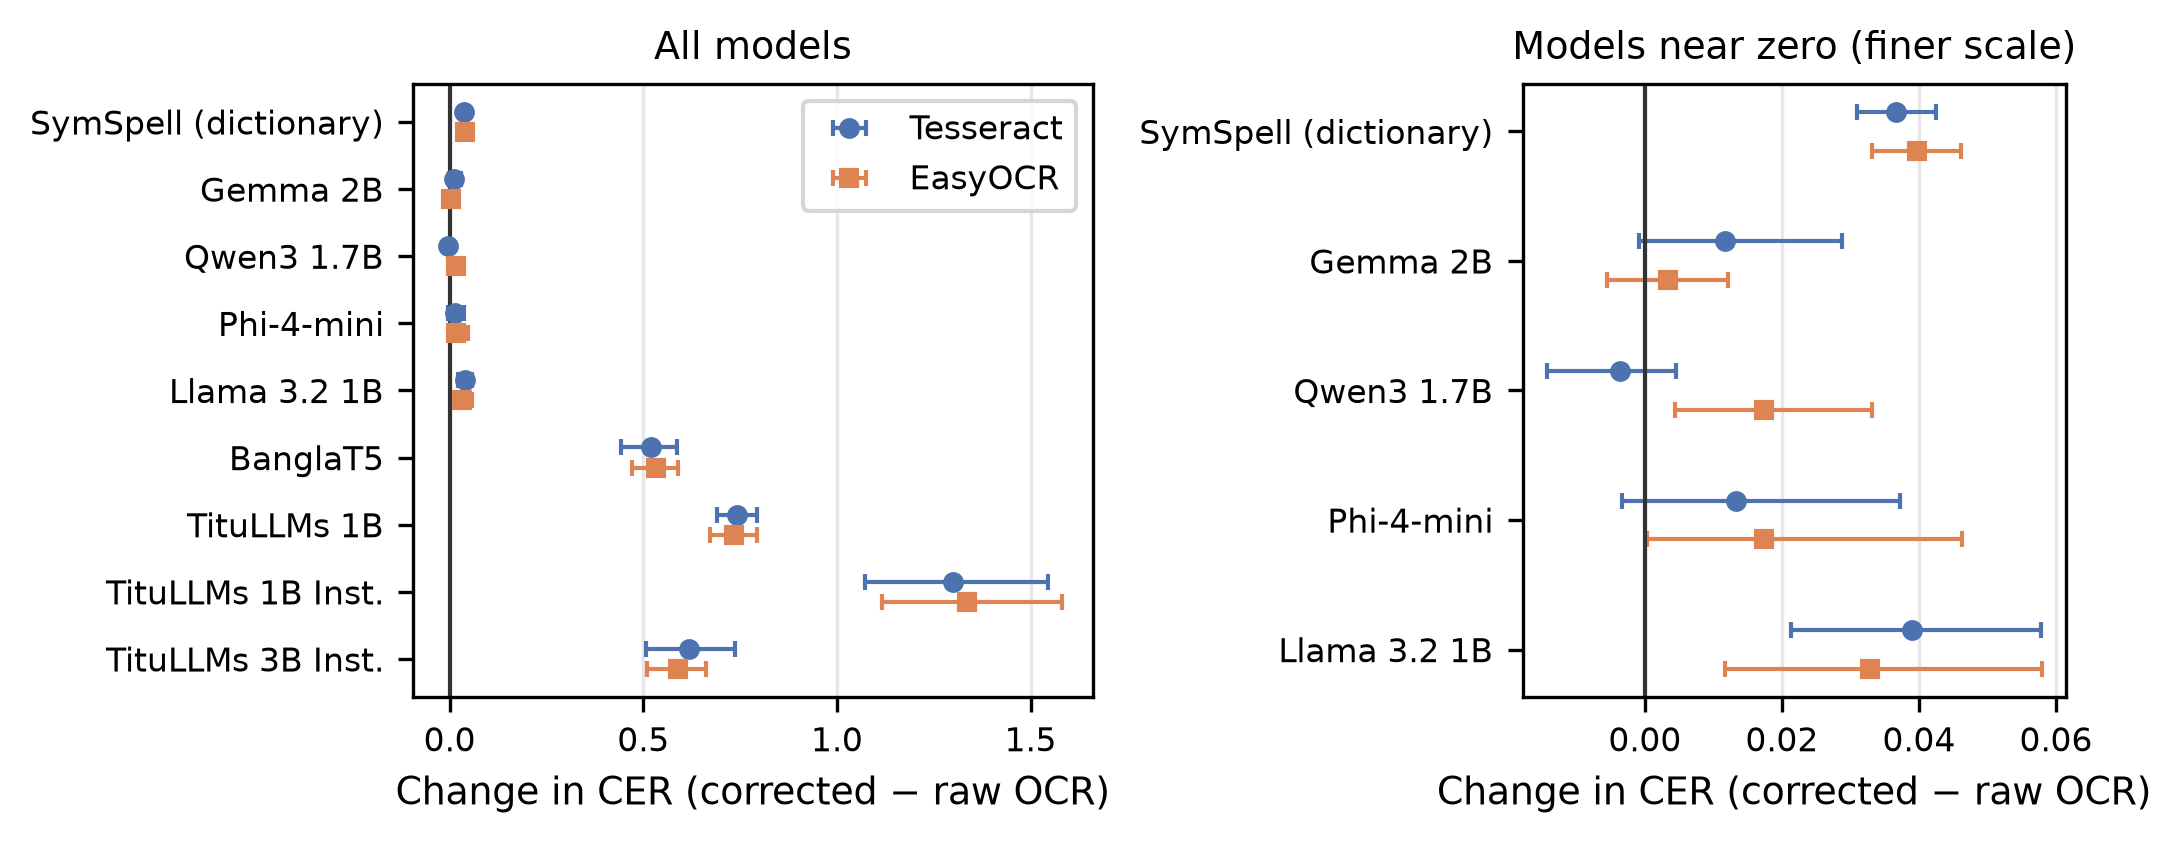
\includegraphics[width=0.85\textwidth]{figures/fig_delta.png}
\caption{Mean change in CER (corrected minus raw OCR) per method and engine, with 95\% paired-bootstrap intervals over the 40 pages. Values above zero mean the correction made the text worse. Left: all methods. Right: the methods near zero on a finer scale.}
\label{fig:delta}
\end{figure*}

\subsubsection{Robustness of the statistics and the reference}
\label{sec:robustness}
The character-level conclusions do not depend on how the error is measured, how pages are resampled, or how the reference is ordered (Table~\ref{tab:robustness}, appendix). The pooled CER is lower than the mean page CER (0.298 against 0.341 for raw Tesseract output, 0.286 against 0.297 for EasyOCR), because short pages have higher error rates, but it ranks the methods in the same way, and on it no method is below the raw OCR. Grapheme-cluster CER improves only for Qwen3 1.7B on Tesseract output, as reported above. On the bounded cMER (Table~\ref{tab:damage}), 13 of the 18 tests are significant after Holm correction, all increases. Resampling whole books instead of pages gives practically the same intervals, as expected with 37 books for 40 pages.

Against a reference rebuilt in the declared reading order, which changes 17 of the 40 references, the raw OCR scores slightly better (CER 0.335 and 0.294 against 0.341 and 0.297), and the same 12 of the 18 CER comparisons are significant, all increases; Qwen3 1.7B on Tesseract output stays at $-0.004$ ($p=0.82$). Reference-word recall, which ignores word order and extra text, is 0.431 and 0.484 for the raw OCR. No method raises it significantly: Qwen3 1.7B comes closest ($+0.003$ and $+0.002$), and every other method lowers it significantly, Gemma-2B-it included ($-0.017$ and $-0.019$). The absence of a significant improvement therefore persists under the declared reading order and under order-free word recall, and also when each region is read separately (Section~\ref{sec:region}).

\subsubsection{Region-level OCR}
\label{sec:region}
Reading each annotated region on its own removes out-of-region text and reading-order differences at the source (Section~\ref{sec:further}), and it lowers the input CER. For EasyOCR, region OCR has CER 0.225 against 0.297 for the whole page read in the same run (paired difference $-0.072$, 95\% CI $[-0.120,-0.033]$); for Tesseract, with whole pages and regions read by the same build in the same run, 0.333 against 0.425 ($-0.092$, $[-0.152,-0.029]$). Correction still does not help (Table~\ref{tab:region}). No method lowers CER on either engine. Every method is significantly worse on EasyOCR text, and on Tesseract text all except Qwen3 1.7B ($+0.015$, $p=0.063$) and Qwen3 4B ($+0.009$, $p=0.19$). On whole-page EasyOCR output only Llama 3.2 1B among the general-purpose models was significantly worse; on region text all of them are, adding 0.009 to 0.066 CER. Phi-4-mini's $+0.066$, the widest interval, is driven by three pages whose output reached the token limit: they account for 87\% of its total increase, one of them alone rose by 1.35. Its median page change is $+0.007$, and it is worse on 30 of the 40 pages. A possible reason is that, with fewer errors to repair, their wrong edits weigh more. The dictionary raises CER by 0.036 and 0.044, and the Bengali-pretrained checkpoints again regenerate the text (CER 0.82 to 1.63). Qwen3 4B lowers WER while raising CER, on EasyOCR text significantly in both directions ($-0.030$ and $+0.014$).

% ---- begin tables/region ----
\begin{table*}[t]
\centering
\caption{Correction of Region-Level OCR (Mean CER and Change, 40 Pages)}
\label{tab:region}
\setlength{\tabcolsep}{4pt}
\footnotesize
\begin{tabular}{lcccccccc}
\toprule
 & \multicolumn{4}{c}{Tesseract} & \multicolumn{4}{c}{EasyOCR} \\
\cmidrule(lr){2-5}\cmidrule(lr){6-9}
Method & CER & $\Delta$CER [95\% CI] & $\Delta$WER & \shortstack{Broken /\\fixed (words)} & CER & $\Delta$CER [95\% CI] & $\Delta$WER & \shortstack{Broken /\\fixed (words)} \\
\midrule
Raw region OCR & 0.333 &  &  &  & 0.225 &  &  &  \\
\midrule
SymSpell (dictionary) & 0.369$^{+}$ & +0.036 [+0.031, +0.041] & +0.108$^{+}$ & 598 / 50 & 0.269$^{+}$ & +0.044 [+0.037, +0.050] & +0.104$^{+}$ & 662 / 150 \\
Gemma-2B-it & 0.349$^{+}$ & +0.016 [+0.006, +0.031] & +0.021$^{+}$ & 127 / 8 & 0.240$^{+}$ & +0.016 [+0.005, +0.034] & +0.008 & 60 / 2 \\
Qwen3 1.7B & 0.347 & +0.015 [+0.005, +0.026] & -0.002 & 125 / 57 & 0.234$^{+}$ & +0.009 [+0.002, +0.019] & -0.012 & 95 / 109 \\
Phi-4-mini & 0.346$^{+}$ & +0.013 [+0.005, +0.023] & +0.007 & 127 / 16 & 0.291$^{+}$ & +0.066 [+0.009, +0.149] & +0.014 & 209 / 24 \\
Llama 3.2 1B & 0.413$^{+}$ & +0.080 [+0.058, +0.104] & +0.027 & 326 / 21 & 0.271$^{+}$ & +0.046 [+0.029, +0.065] & +0.014 & 169 / 36 \\
BanglaT5 & 0.883$^{+}$ & +0.551 [+0.466, +0.619] & +0.349$^{+}$ & 2114 / 30 & 0.846$^{+}$ & +0.622 [+0.581, +0.665] & +0.490$^{+}$ & 2103 / 90 \\
TituLLMs 1B & 0.905$^{+}$ & +0.573 [+0.512, +0.630] & +0.532$^{+}$ & 1627 / 93 & 0.985$^{+}$ & +0.761 [+0.713, +0.803] & +0.685$^{+}$ & 1619 / 101 \\
TituLLMs 1B Instruct & 1.629$^{+}$ & +1.296 [+1.060, +1.593] & +1.637$^{+}$ & 1570 / 40 & 1.596$^{+}$ & +1.371 [+1.228, +1.516] & +1.622$^{+}$ & 1739 / 36 \\
TituLLMs 3B Instruct & 0.901$^{+}$ & +0.568 [+0.466, +0.675] & +0.372$^{+}$ & 2080 / 4 & 0.824$^{+}$ & +0.599 [+0.520, +0.667] & +0.308$^{+}$ & 2000 / 2 \\
Qwen3 4B & 0.342 & +0.009 [-0.001, +0.021] & -0.015 & 158 / 173 & 0.239$^{+}$ & +0.014 [+0.005, +0.023] & -0.030$^{-}$ & 121 / 217 \\
\bottomrule
\end{tabular}
\par\smallskip
\begin{minipage}{\linewidth}\footnotesize Each PAGE-XML text region read separately (576 regions with text) and scored against the regions in reading order. Whole-page OCR from the same run: Tesseract 0.425, EasyOCR 0.297; region OCR changes them by -0.092 [-0.152, -0.029] and -0.072 [-0.120, -0.033] (paired bootstrap). The Tesseract build of this run does not reproduce the main run's text (CER 0.22 between them), so Tesseract region results are compared only within this run; EasyOCR reproduces the main run (CER 0.002 between them). $\Delta$: corrected $-$ raw region OCR (positive = worse). $^{+}$/$^{-}$: significantly higher/lower, Wilcoxon signed-rank, Holm-corrected over the 20 cells of the table for each metric (exploratory). Broken / fixed: reference words the raw OCR had right that the output gets wrong, and words it had wrong that the output gets right, as counts of the 4{,}497 aligned reference words, so the two can be compared directly.\end{minipage}
\end{table*}
% ---- end tables/region ----

\subsubsection{Synthetic noise}
\label{sec:noise}
If the OCR were simply too noisy to correct, correction should start to help as the noise falls. It does not (Table~\ref{tab:noise}, Fig.~\ref{fig:noise}). On references corrupted to mean CERs of 0.020, 0.048, 0.100, 0.199 and 0.297, each of the four general-purpose models raised the CER at every level, and all 20 increases are significant. Only at the highest level (0.297) did two models lower the word error rate significantly, Llama 3.2 1B by 0.006 and Phi-4-mini by 0.018, while still raising CER. No tested noise level produced a CER reduction: at an input CER of 0.020 the corrected text has CER 0.044 to 0.107, two to five times the input. Gemma-2B-it adds the least, 0.016 to 0.034, and Llama 3.2 1B the most, 0.087 to 0.169 (computed from unrounded values, so differences of the rounded table entries can differ by 0.001). The synthetic noise is not a perfect stand-in for real OCR errors: at the same input CER of about 0.30, the models leave synthetic noise worse than real EasyOCR output (Qwen3 1.7B: 0.362 against 0.315), so the sweep shows the trend, not the exact level a real OCR text would reach.

\begin{figure}[t]
\centering
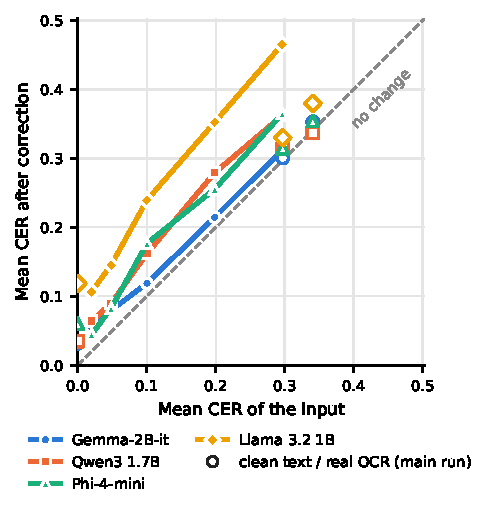
\includegraphics[width=0.85\columnwidth]{figures/fig_noise.pdf}
\caption{Mean CER after correction against mean CER of the input for the four general-purpose models. Lines: the 40 references corrupted with synthetic OCR noise at five levels. Open markers: the clean-text control (input CER 0) and the real OCR of the two engines in the main run. Points above the dashed line are made worse by the correction.}
\label{fig:noise}
\end{figure}

% ---- begin tables/noise ----
\begin{table}[t]
\centering
\caption{Correction of Synthetic Noise (Mean CER After Correction)}
\label{tab:noise}
\setlength{\tabcolsep}{4pt}
\footnotesize
\begin{tabular}{lccccc}
\toprule
Input CER & 0.020 & 0.048 & 0.100 & 0.199 & 0.297 \\
\midrule
Gemma-2B-it & 0.054$^{+}$ & 0.080$^{+}$ & 0.119$^{+}$ & 0.215$^{+}$ & 0.312$^{+}$ \\
Qwen3 1.7B & 0.064$^{+}$ & 0.090$^{+}$ & 0.162$^{+}$ & 0.279$^{+}$ & 0.362$^{+}$ \\
Phi-4-mini & 0.044$^{+}$ & 0.083$^{+}$ & 0.177$^{+}$ & 0.256$^{+}$ & 0.365$^{+}$ \\
Llama 3.2 1B & 0.107$^{+}$ & 0.145$^{+}$ & 0.239$^{+}$ & 0.352$^{+}$ & 0.465$^{+}$ \\
\bottomrule
\end{tabular}
\par\smallskip
\begin{minipage}{\linewidth}\footnotesize The 40 references corrupted with a character-level noise model estimated from the OCR of the 10 development pages only, scaled to each target CER. $^{+}$/$^{-}$: higher/lower than the input, Wilcoxon signed-rank, Holm-corrected over the 20 cells (exploratory).\end{minipage}
\end{table}
% ---- end tables/noise ----

\subsubsection{Model size}
\label{sec:scale}
Table~\ref{tab:scale} adds six general-purpose models to the four of the main runs: Qwen3 at 0.6, 4 and 8 billion parameters, Gemma~3 at 1 and 4 billion, and Llama 3.2 3B. None lowers CER on either engine. More parameters do not help consistently within a family: Gemma~3 4B damages more than Gemma~3 1B ($+0.062$ against $+0.022$ on Tesseract text), while Llama 3.2 3B stays close to the raw OCR where Llama 3.2 1B was significantly worse. Qwen3 is the only family in which size moves correction towards improvement. Of the 4{,}497 aligned reference words, Qwen3 0.6B breaks 349 correct words and fixes 100 on Tesseract text, whereas the 4B and 8B models fix more than they break (209 and 263 fixed against 104 and 112 broken; on EasyOCR text 201 and 340 against 100 and 113), and their WER falls significantly (by 0.021 to 0.065). Their CER does not fall (changes of $+0.003$ and $+0.004$, not significant), so the extra repaired words do not show at the character level; Section~\ref{sec:editlevel} shows which edits account for this. Every model also changes error-free input (CER 0.024 to 0.212).

% ---- begin tables/scale ----
\begin{table*}[t]
\centering
\caption{General-Purpose Models by Family and Size (Change Against Raw OCR, 40 Pages)}
\label{tab:scale}
\setlength{\tabcolsep}{4pt}
\footnotesize
\begin{tabular}{lccccccc}
\toprule
 & \multicolumn{2}{c}{$\Delta$CER} & Clean text & \multicolumn{2}{c}{$\Delta$WER} & \multicolumn{2}{c}{Broken / fixed (words)} \\
\cmidrule(lr){2-3}\cmidrule(lr){4-4}\cmidrule(lr){5-6}\cmidrule(lr){7-8}
Model & Tesseract & EasyOCR & CER & Tesseract & EasyOCR & Tesseract & EasyOCR \\
\midrule
Qwen3 0.6B & +0.043 & +0.065$^{+}$ & 0.212 & -0.048 & +0.012 & 349 / 100 & 377 / 104 \\
Qwen3 1.7B$^{\dagger}$ & -0.004 & +0.017 & 0.035 & -0.028$^{-}$ & +0.013 & 65 / 83 & 95 / 89 \\
Qwen3 4B & +0.003 & +0.004 & 0.032 & -0.021$^{-}$ & -0.032$^{-}$ & 104 / 209 & 100 / 201 \\
Qwen3 8B & +0.004 & +0.003 & 0.029 & -0.029$^{-}$ & -0.065$^{-}$ & 112 / 263 & 113 / 340 \\
Gemma-2B-it$^{\dagger}$ & +0.012 & +0.003 & 0.032 & +0.002 & -0.001 & 77 / 11 & 72 / 12 \\
Gemma 3 1B & +0.022$^{+}$ & +0.029$^{+}$ & 0.024 & -0.027 & +0.036 & 185 / 20 & 181 / 13 \\
Gemma 3 4B & +0.062$^{+}$ & +0.057$^{+}$ & 0.069 & -0.014 & -0.020 & 439 / 181 & 314 / 227 \\
Llama 3.2 1B$^{\dagger}$ & +0.039$^{+}$ & +0.033$^{+}$ & 0.119 & -0.023 & -0.009 & 214 / 33 & 156 / 38 \\
Llama 3.2 3B & +0.016 & +0.004 & 0.059 & -0.014 & -0.033$^{-}$ & 143 / 72 & 126 / 137 \\
Phi-4-mini$^{\dagger}$ & +0.013 & +0.017 & 0.060 & -0.005 & +0.005 & 192 / 33 & 207 / 42 \\
\bottomrule
\end{tabular}
\par\smallskip
\begin{minipage}{\linewidth}\footnotesize $\Delta$: corrected $-$ raw OCR (positive = worse); clean text: CER of the output when the reference itself is the input. $^{\dagger}$: core models of the main runs; the others extend the comparison to newer checkpoints and to size within the Qwen3, Gemma and Llama families (same prompt, chunking and plain decoding; float16 above 3B parameters, Gemma 3 in float32). $^{+}$/$^{-}$: Holm-significant, Wilcoxon signed-rank, within each run's exploratory family (main run 24 cells, added models 18 cells, per metric). Broken / fixed: reference words the raw OCR had right that the output gets wrong, and words it had wrong that the output gets right, as counts of the 4{,}497 aligned reference words, so the two can be compared directly.\end{minipage}
\end{table*}
% ---- end tables/scale ----

On the 10 pages of the attribution analysis, Qwen3 32B in 4-bit continues the trend (Table~\ref{tab:large}). Of the 1{,}292 aligned reference words on these pages it fixes 91 and 139 wrong words, the most of any model, against 48 and 62 correct words broken, and lowers WER by 0.092 and 0.110. Its CER changes, $-0.003$ (95\% CI $[-0.015,+0.010]$) and $-0.006$ ($[-0.035,+0.019]$), are indistinguishable from zero. On error-free input it does more damage than Qwen3 1.7B, 4B or 8B on the same pages (CER 0.073 against 0.011 to 0.028). The Holm family for this subset is all 12 models rescored on the 10 pages (the eight core models and the four Qwen3 sizes) on three inputs, 36 comparisons per metric, of which the table shows the Qwen3 rows. This subset provides descriptive effect estimates; under the specified multiplicity correction, the tests cannot reach the significance threshold. A model nearly 20 times the size of the main runs' Qwen3 fixes more words than it breaks, but its CER does not fall measurably.

% ---- begin tables/large ----
\begin{table}[t]
\centering
\caption{Qwen3 from 0.6B to 32B Parameters on 10 Pages (Change Against the Input)}
\label{tab:large}
\setlength{\tabcolsep}{3pt}
\footnotesize
\begin{tabular}{lccccc}
\toprule
 & \multicolumn{3}{c}{$\Delta$CER} & \multicolumn{2}{c}{$\Delta$WER} \\
\cmidrule(lr){2-4}\cmidrule(lr){5-6}
Model & Tess. & Easy. & Clean & Tess. & Easy. \\
\midrule
Qwen3 0.6B & +0.008 & +0.095 & +0.194 & -0.063 & +0.109 \\
Qwen3 1.7B & +0.004 & +0.031 & +0.011 & -0.042 & +0.070 \\
Qwen3 4B & +0.007 & +0.001 & +0.021 & -0.016 & -0.021 \\
Qwen3 8B & +0.004 & -0.001 & +0.028 & -0.035 & -0.061 \\
Qwen3 32B (4-bit) & -0.003 & -0.006 & +0.073 & -0.092 & -0.110 \\
\bottomrule
\end{tabular}
\par\smallskip
\begin{minipage}{\linewidth}\footnotesize The 10 pages of the attribution analysis (raw CER 0.377 Tesseract, 0.272 EasyOCR). Qwen3 32B in 4-bit (NF4) on two T4 GPUs; the others as in Table~\ref{tab:scale}, restricted to the same pages. Tests: Wilcoxon signed-rank, Holm-corrected over the 36 cells of each metric, that is, all 12 models rescored on these pages (the 8 core models and Qwen3 0.6B, Qwen3 4B, Qwen3 8B, Qwen3 32B (4-bit)) on the 3 inputs; the table shows the Qwen3 rows. With 10 pages the smallest possible two-sided Wilcoxon $p$ is $2/2^{10}$, so after this correction no change can reach significance (smallest adjusted $p$ 0.070): the table gives descriptive estimates, and the text gives 95\% intervals.\end{minipage}
\end{table}
% ---- end tables/large ----

\subsubsection{Fine-tuning pilot}
\label{sec:finetune}
A small model trained for the task behaves much like the larger zero-shot Qwen3 models (Table~\ref{tab:finetune}). The fine-tuned ByT5-small lowers WER significantly on both engines, by 0.024 and 0.037; it fixes 113 and 282 wrong words while breaking 102 and 146 correct ones. CER does not fall. It rises by 0.012 on Tesseract text, significantly, with 25 of the 40 pages worse, and by 0.016 on EasyOCR text, where the bootstrap interval excludes zero but the Holm-corrected test is not significant. On error-free input it does less damage than any other method run on the 40 pages: CER 0.015, against 0.017 for the best dictionary setting and 0.032 for Gemma-2B-it. The checkpoint chosen on the development pages also stayed just above their raw OCR (CER 0.365 against 0.362). This is a preliminary pilot: the model saw about 14{,}300 of its 43{,}312 training pairs, once each, before the time budget ran out. It shows only that this short training produced copy-and-edit behaviour, not how well a fully trained model would correct.

% ---- begin tables/finetune ----
\begin{table*}[t]
\centering
\caption{Fine-Tuning Pilot: ByT5-Small Trained on Synthetic OCR Noise (40 Pages)}
\label{tab:finetune}
\setlength{\tabcolsep}{4pt}
\footnotesize
\begin{tabular}{lccccccc}
\toprule
Input & Raw CER & Corrected CER & $\Delta$CER [95\% CI] & $\Delta$WER & \shortstack{Broken /\\fixed (words)} & \shortstack{Pages better /\\worse} & Truncated \\
\midrule
Tesseract & 0.341 & 0.353$^{+}$ & +0.012 [-0.001, +0.026] & -0.024$^{-}$ & 102 / 113 & 11/25 & 5 \\
EasyOCR & 0.297 & 0.313 & +0.016 [+0.001, +0.034] & -0.037$^{-}$ & 146 / 282 & 19/19 & 5 \\
Clean text & 0.000 & 0.015$^{+}$ & +0.015 [+0.009, +0.023] & +0.051$^{+}$ & 196 / -- & 0/33 & 1 \\
\bottomrule
\end{tabular}
\par\smallskip
\begin{minipage}{\linewidth}\footnotesize google/byt5-small fine-tuned on Bengali Wikipedia segments and development-page reference lines, corrupted with the development-page noise model (no evaluation text in training). Training: 43{,}312 training pairs, 1{,}793 updates of 8 pairs (155 min on one T4 GPU, including the development evaluations); development-page CER 0.365 after correction against 0.362 raw (checkpoint chosen on it). $^{+}$/$^{-}$: Holm-significant over the 3 cells (exploratory). Broken / fixed: reference words the raw OCR had right that the output gets wrong, and words it had wrong that the output gets right, as counts of the 4{,}497 aligned reference words, so the two can be compared directly.\end{minipage}
\end{table*}
% ---- end tables/finetune ----

\subsubsection{Methods without a language model}
\label{sec:classical}
Two further methods use no language model (Table~\ref{tab:classical}). A better lexicon and a smaller edit distance reduce the dictionary's damage but do not remove it. The 100{,}000 most frequent words of Bengali Wikipedia miss 37\% of the reference word tokens, against 52\% for the subtitle lexicon. With this lexicon and an edit distance of 1, SymSpell raises CER by 0.007 and 0.008 instead of 0.037 and 0.040, and error-free text reaches CER 0.017 instead of 0.057. Every setting nevertheless remains significantly worse than the raw OCR on both engines: the best one still breaks 211 and 251 correct words and fixes 88 and 201 wrong ones.

Engine fusion combines the two readings instead of correcting one. With EasyOCR as the base and Tesseract's reading taken where its confidence ranks higher, CER falls from 0.297 to 0.294 and 0.295 for the two rules, and WER falls by 0.014 (significant for both). Like the larger Qwen3 models and the fine-tuned model, fusion fixes more words than it breaks (140 against 71, and 87 against 30), and the margin rule breaks fewer correct words than any language model without gating on the 40 pages. Its CER gain is small, 1.1\% and 0.8\% of the raw CER, and we report it as descriptive, not significant. Only the margin rule's change ($-0.002$) reaches $p<0.05$, and only after Holm correction over the two comparisons with EasyOCR ($p=0.045$); over the four comparisons of the first scoring, which also compared fusion with Tesseract output, it does not ($p=0.090$). We chose the smaller family after seeing that result, because a comparison with Tesseract output mostly measures the difference between the engines, so the $p=0.045$ cannot count as a confirmed effect.

% ---- begin tables/classical ----
\begin{table*}[t]
\centering
\caption{Methods Without a Language Model: Dictionary Variants and Engine Fusion (40 Pages)}
\label{tab:classical}
\setlength{\tabcolsep}{4pt}
\footnotesize
\begin{tabular}{lccccccc}
\toprule
 & \multicolumn{2}{c}{$\Delta$CER [95\% CI]} & Clean text & \multicolumn{2}{c}{$\Delta$WER} & \multicolumn{2}{c}{Broken / fixed (words)} \\
\cmidrule(lr){2-3}\cmidrule(lr){4-4}\cmidrule(lr){5-6}\cmidrule(lr){7-8}
Method & Tesseract & EasyOCR & CER & Tesseract & EasyOCR & Tesseract & EasyOCR \\
\midrule
SymSpell, subtitles, $d\le2$ (main) & +0.037$^{+}$ [+0.031, +0.042] & +0.040$^{+}$ [+0.033, +0.046] & 0.057 & +0.091$^{+}$ & +0.095$^{+}$ & 563 / 74 & 605 / 175 \\
SymSpell, subtitles, $d\le1$ & +0.016$^{+}$ [+0.013, +0.020] & +0.017$^{+}$ [+0.014, +0.021] & 0.025 & +0.062$^{+}$ & +0.057$^{+}$ & 408 / 60 & 425 / 168 \\
SymSpell, Wikipedia, $d\le2$ & +0.017$^{+}$ [+0.012, +0.022] & +0.021$^{+}$ [+0.016, +0.026] & 0.039 & +0.031$^{+}$ & +0.030$^{+}$ & 309 / 112 & 377 / 218 \\
SymSpell, Wikipedia, $d\le1$ & +0.007$^{+}$ [+0.004, +0.010] & +0.008$^{+}$ [+0.006, +0.011] & 0.017 & +0.019$^{+}$ & +0.012 & 211 / 88 & 251 / 201 \\
\midrule
Fusion, higher confidence & -- & -0.003 [-0.007, -0.001] & -- & -- & -0.014$^{-}$ & -- & 71 / 140 \\
Fusion, confidence margin & -- & -0.002 [-0.005, -0.000] & -- & -- & -0.014$^{-}$ & -- & 30 / 87 \\
\bottomrule
\end{tabular}
\par\smallskip
\begin{minipage}{\linewidth}\footnotesize $\Delta$: output $-$ raw OCR of that engine (positive = worse). SymSpell: lexicon of the 50{,}000 most frequent OpenSubtitles words (main baseline) or of the most frequent words of Bengali Wikipedia; $d$: maximum edit distance. Fusion: EasyOCR text in which short stretches where the engines disagree take Tesseract's reading if its confidence ranks higher within the page (margin: by at least 0.25); it is compared with EasyOCR, its base, only, and needs two OCR readings, so it has no clean-text control. $^{+}$/$^{-}$: Holm-significant, Wilcoxon signed-rank, over the 12 dictionary cells and, separately, the 2 fusion cells, per metric (exploratory). Fusion CER changes are descriptive, not significant. Holm-adjusted Wilcoxon $p$ over the 2 fusion cells / over the 4 cells of the first scoring, which added the comparisons with Tesseract output (the smaller family was chosen after it): higher-confidence rule 0.068 / 0.205; margin rule 0.045 / 0.090. Broken / fixed: reference words the raw OCR had right that the output gets wrong, and words it had wrong that the output gets right, as counts of the 4{,}497 aligned reference words, so the two can be compared directly.\end{minipage}
\end{table*}
% ---- end tables/classical ----

\subsection{RQ2: Preservation and repair}
\label{sec:rq2}

\subsubsection{Clean-text control}
\label{sec:clean}
Giving the models reference text removes any recognition error they could repair. Nevertheless, every method changes it (Table~\ref{tab:clean}). Among the core methods, Gemma-2B-it and Qwen3 1.7B do the least damage, with CER 0.032 and 0.035, leaving 6 and 2 of the 40 pages exactly unchanged. The corresponding CERs are 0.060 for Phi-4-mini, 0.057 for the dictionary baseline and 0.119 for Llama 3.2 1B. The dictionary replaces about 31 correct words per page, giving WER 0.268. The Bengali-pretrained checkpoints reach CERs of 0.83 to 1.57 despite the error-free input. These changes are over-correction by construction; their magnitude gives nearly the same ordering of methods as the main evaluation. Phi-4-mini's pooled CER (0.097) is far above its mean (0.060) because of one long page: partway through a chunk its output switches to English prose about physical properties of an object and runs to the token limit, at 1.94 times the reference length, which gives 70\% of its character errors on the 40 pages.

% ---- begin tables/clean ----
\begin{table}[t]
\centering
\caption{Clean-Text Control: Ground Truth Given as Input}
\label{tab:clean}
\setlength{\tabcolsep}{3pt}
\footnotesize
\begin{tabular}{lccccc}
\toprule
Model & \shortstack{Mean\\CER} & \shortstack{Pooled\\CER} & WER & wMER & \shortstack{Pages\\unchanged} \\
\midrule
SymSpell (dictionary) & 0.057 & 0.057 & 0.268 & 0.268 & 0/40 \\
Gemma-2B-it & 0.032 & 0.028 & 0.097 & 0.096 & 6/40 \\
Qwen3 1.7B & 0.035 & 0.031 & 0.156 & 0.154 & 2/40 \\
Phi-4-mini & 0.060 & 0.097 & 0.148 & 0.132 & 4/40 \\
Llama 3.2 1B & 0.119 & 0.118 & 0.163 & 0.157 & 3/40 \\
BanglaT5 & 0.833 & 0.837 & 1.059 & 0.937 & 0/40 \\
TituLLMs 1B & 0.988 & 0.976 & 1.341 & 0.810 & 0/40 \\
TituLLMs 1B Instruct & 1.565 & 1.554 & 2.129 & 0.891 & 0/40 \\
TituLLMs 3B Instruct & 0.967 & 0.954 & 1.173 & 0.927 & 0/40 \\
\bottomrule
\end{tabular}
\par\smallskip
\begin{minipage}{\linewidth}\footnotesize Each model receives the reference text itself, with the same prompt and plain decoding. Error rates are measured against that reference, so any value above 0 is damage to correct text; WER and wMER are per-page means. Pages unchanged: CER exactly 0 after normalisation.\end{minipage}
\end{table}
% ---- end tables/clean ----

\subsubsection{Words fixed and broken}
Table~\ref{tab:diagnostics} reports how many ground-truth words each output retains. Raw Tesseract output keeps 46\% of the distinct ground-truth words and raw EasyOCR output 53\%. Averaged over the outputs of both engines, the general-purpose models keep 46\% to 49\%, the dictionary baseline 37\%, and the Bengali-pretrained checkpoints between 3\% and 16\%. The script shares in the same table are pooled over all output characters, so they describe the text a method produced, not how often it produced any: the output of TituLLMs 3B Instruct is 97\% Bengali, but 27 of its 80 outputs are empty. Table~\ref{tab:damage} separates correct words that were changed from wrong words that were fixed, each as a share of its own group (words the raw OCR had right, words it had wrong), so the two shares cannot be compared with each other; counts of the same 4{,}497 reference words can (Table~\ref{tab:scale}). Gemma-2B-it broke 77 and 72 correct words and fixed 11 and 12. Qwen3 1.7B broke 65 and 95 and fixed 83 and 89, the only core model to fix more words than it broke, and only on Tesseract text. Phi-4-mini and Llama 3.2 1B broke 8\% to 11\% of the correct words, the dictionary baseline 29\% and 31\%, and the Bengali-pretrained checkpoints between 74\% and 99\%. The change ratio is below 1 for the general-purpose models and the dictionary (0.1 to 0.4) and between 3.9 and 7.0 for the Bengali-pretrained checkpoints.

% ---- begin tables/diagnostics ----
\begin{table}[t]
\centering
\caption{Output Diagnostics by Model}
\label{tab:diagnostics}
\setlength{\tabcolsep}{3pt}
\footnotesize
\begin{tabular}{lcccccc}
\toprule
Source & Len. & Bn & Latin & Other & GT ret. & Empty \\
\midrule
Raw Tesseract & 1.03$\times$ & 93\% & 0\% & 7\% & 46\% & 0/40 \\
Raw EasyOCR & 1.02$\times$ & 92\% & 0\% & 8\% & 53\% & 0/40 \\
\midrule
SymSpell (dictionary) & \best{1.00$\times$} & 93\% & \best{0\%} & 7\% & 37\% & 0/80 \\
Gemma-2B-it & 1.00$\times$ & 92\% & \best{0\%} & 8\% & 47\% & 0/80 \\
Qwen3 1.7B & 1.01$\times$ & 93\% & \best{0\%} & 7\% & \best{49\%} & 0/80 \\
Phi-4-mini & 1.00$\times$ & 92\% & 1\% & 7\% & 46\% & 0/80 \\
Llama 3.2 1B & 0.94$\times$ & 94\% & \best{0\%} & 6\% & 46\% & 0/80 \\
BanglaT5 & 0.45$\times$ & 72\% & 0\% & 28\% & 3\% & 0/80 \\
TituLLMs 1B & 1.50$\times$ & \best{97\%} & \best{0\%} & \best{3\%} & 16\% & 0/80 \\
TituLLMs 1B Instruct & 2.09$\times$ & 88\% & 5\% & 7\% & 13\% & 0/80 \\
TituLLMs 3B Instruct & 0.50$\times$ & 97\% & 0\% & 3\% & 4\% & 27/80 \\
\bottomrule
\end{tabular}
\par\smallskip
\begin{minipage}{\linewidth}\footnotesize Both engines together (80 outputs per model; 40 per raw OCR row). Len.: output length / reference length, mean over outputs (the raw OCR values are those of Table~\ref{tab:dataset}). Bn / Latin / Other: share of all non-space output characters, pooled over outputs, so empty outputs do not enter. GT ret.: share of distinct ground-truth words present in the output, mean over outputs (an empty output retains none). Empty: outputs with no text.\end{minipage}
\end{table}
% ---- end tables/diagnostics ----

% ---- begin tables/damage ----
\begin{table*}[t]
\centering
\caption{What Correction Changed: Bounded Error, Word-Level Damage and Fixes, and Change Ratio}
\label{tab:damage}
\setlength{\tabcolsep}{4pt}
\footnotesize
\begin{tabular}{llccccc}
\toprule
Engine & Model & cMER & \shortstack{Correct words\\broken} & \shortstack{Wrong words\\fixed} & \shortstack{Change\\ratio} & \shortstack{Invented\\runs} \\
\midrule
Tesseract & (no correction) & 0.290 & --- & --- & --- & --- \\
Tesseract & SymSpell (dictionary) & 0.325$^{+}$ & 29\% & 2.9\% & 0.3 & \best{0\%} \\
Tesseract & Gemma-2B-it & 0.303 & 4\% & 0.4\% & \best{0.2} & \best{0\%} \\
Tesseract & Qwen3 1.7B & \best{0.292} & \best{3\%} & 3.3\% & 0.2 & 0\% \\
Tesseract & Phi-4-mini & 0.305 & 10\% & 1.3\% & 0.2 & 1\% \\
Tesseract & Llama 3.2 1B & 0.338$^{+}$ & 11\% & 1.3\% & 0.4 & 0\% \\
Tesseract & BanglaT5 & 0.847$^{+}$ & 96\% & 1.8\% & 4.1 & 0\% \\
Tesseract & TituLLMs 1B & 0.705$^{+}$ & 74\% & \best{4.6\%} & 4.9 & 14\% \\
Tesseract & TituLLMs 1B Instruct & 0.744$^{+}$ & 79\% & 1.5\% & 6.9 & 33\% \\
Tesseract & TituLLMs 3B Instruct & 0.845$^{+}$ & 96\% & 0.3\% & 4.5 & 9\% \\
\midrule
EasyOCR & (no correction) & 0.260 & --- & --- & --- & --- \\
EasyOCR & SymSpell (dictionary) & 0.300$^{+}$ & 31\% & \best{6.9\%} & 0.4 & \best{0\%} \\
EasyOCR & Gemma-2B-it & \best{0.264} & \best{4\%} & 0.5\% & \best{0.1} & \best{0\%} \\
EasyOCR & Qwen3 1.7B & 0.275 & 5\% & 3.5\% & 0.2 & 0\% \\
EasyOCR & Phi-4-mini & 0.279$^{+}$ & 11\% & 1.6\% & 0.2 & 0\% \\
EasyOCR & Llama 3.2 1B & 0.298$^{+}$ & 8\% & 1.5\% & 0.4 & 0\% \\
EasyOCR & BanglaT5 & 0.828$^{+}$ & 99\% & 2.3\% & 3.9 & \best{0\%} \\
EasyOCR & TituLLMs 1B & 0.677$^{+}$ & 76\% & 4.8\% & 4.6 & 13\% \\
EasyOCR & TituLLMs 1B Instruct & 0.749$^{+}$ & 78\% & 2.2\% & 7.0 & 30\% \\
EasyOCR & TituLLMs 3B Instruct & 0.845$^{+}$ & 95\% & 0.3\% & 4.1 & 2\% \\
\bottomrule
\end{tabular}
\par\smallskip
\begin{minipage}{\linewidth}\footnotesize cMER $=(S{+}D{+}I)/(H{+}S{+}D{+}I)$, bounded in $[0,1]$. Correct words broken: share of ground-truth words the raw OCR had right that the output gets wrong; wrong words fixed: share the raw OCR had wrong that the output gets right (word alignment against the ground truth). Change ratio: CER of the output against the raw OCR, divided by the raw OCR's CER. Invented runs: share of output characters in runs of $\geq$6 characters with no counterpart in the raw OCR. $^{+}$/$^{-}$: cMER significantly higher/lower than the raw OCR, Wilcoxon signed-rank test, Holm-corrected over the 18 cMER tests (exploratory family). \colorbox{bestbg}{\textbf{Shaded}}: best corrected model per engine.\end{minipage}
\end{table*}
% ---- end tables/damage ----

\subsubsection{Where the character errors go}
\label{sec:editlevel}
Table~\ref{tab:editlevel} splits the change in character errors between the reference words a method fixes, those it breaks, those that stay wrong, and the spaces between words. A fixed word usually saves about one character error: Qwen3 4B and 8B remove 185 to 416 errors by fixing 201 to 340 words, mostly in vowel signs and punctuation. The cost lies elsewhere. The same models edit 394 to 667 words that stay wrong and add 159 to 255 character errors to them, mostly consonants, and the words they break add 89 to 157 more. These costs match or exceed the savings (net $+54$ to $+189$ errors over 29{,}599 reference characters), so CER does not fall, while WER falls because it counts only whether a word is entirely right. The fine-tuned pilot shows the same pattern with larger costs. Merged and split words are not the explanation: with all spaces removed before scoring, every CER moves by at most 0.02 and keeps its direction relative to the raw OCR. Engine fusion is the exception: it removes errors from words that stay wrong instead of adding them, which is why it lowers CER slightly.

% ---- begin tables/editlevel ----
\begin{table*}[t]
\centering
\caption{Where the Character Errors Go: Change in Character Errors by Reference-Word Group (40 Pages, Pooled)}
\label{tab:editlevel}
\setlength{\tabcolsep}{4pt}
\footnotesize
\begin{tabular}{lccccccc}
\toprule
Method & \shortstack{Words\\fixed / broken} & \shortstack{$\Delta$ errors,\\fixed words} & \shortstack{$\Delta$ errors,\\broken words} & \shortstack{$\Delta$ errors, still-wrong\\words (words edited)} & \shortstack{$\Delta$ errors,\\spaces and other} & \shortstack{$\Delta$ errors,\\total} & \shortstack{CER without spaces\\raw / corrected} \\
\midrule
\multicolumn{8}{l}{\textit{Tesseract}} \\
Qwen3 1.7B & 83 / 65 & -83 & +63 & +95 (293) & -55 & +20 & 0.340 / 0.338 \\
Qwen3 4B & 209 / 104 & -187 & +137 & +201 (559) & +38 & +189 & 0.340 / 0.343 \\
Qwen3 8B & 263 / 112 & -243 & +157 & +241 (667) & -46 & +109 & 0.340 / 0.345 \\
Llama 3.2 3B & 72 / 143 & -54 & +207 & +304 (620) & +187 & +644 & 0.340 / 0.360 \\
ByT5-small, fine-tuned & 113 / 102 & -73 & +114 & +187 (597) & +97 & +325 & 0.340 / 0.353 \\
\midrule
\multicolumn{8}{l}{\textit{EasyOCR}} \\
Qwen3 1.7B & 89 / 95 & -46 & +287 & +288 (248) & +53 & +582 & 0.303 / 0.320 \\
Qwen3 4B & 201 / 100 & -185 & +89 & +159 (394) & +87 & +150 & 0.303 / 0.306 \\
Qwen3 8B & 340 / 113 & -416 & +154 & +255 (622) & +61 & +54 & 0.303 / 0.304 \\
Llama 3.2 3B & 137 / 126 & -142 & +100 & +249 (481) & +44 & +251 & 0.303 / 0.308 \\
ByT5-small, fine-tuned & 282 / 146 & -286 & +255 & +399 (584) & +159 & +527 & 0.303 / 0.319 \\
Fusion, higher confidence & 140 / 71 & -163 & +86 & -46 (152) & +28 & -95 & 0.303 / 0.299 \\
\bottomrule
\end{tabular}
\par\smallskip
\begin{minipage}{\linewidth}\footnotesize Each character error of the alignment with the reference is assigned to a reference word (insertions to the word they follow); $\Delta$: errors in the corrected text minus errors in the raw OCR, summed over the 40 pages (29{,}599 reference characters per engine), so the groups add up to the total. Fixed / broken: reference words the output gets right that the raw OCR had wrong, and the reverse. Still wrong: wrong in both; in brackets, how many of them the method edited. Spaces and other: errors on the spaces between words (merged or split words) and insertions next to words that stay right. CER without spaces: mean page CER with all spaces removed. Descriptive, no test.\end{minipage}
\end{table*}
% ---- end tables/editlevel ----

\subsubsection{Examples}
Table~\ref{tab:editops} counts substitutions, deletions and insertions per page against the reference; Table~\ref{tab:examples} shows the outputs for two reference lines. In the first example, Gemma-2B-it and Llama 3.2 1B reproduce the Tesseract text unchanged. Qwen3 1.7B repairs a broken word, while the dictionary modernises a historical form. The Bengali-pretrained checkpoints return unrelated text or nothing. In the second example, Qwen3 1.7B repairs one word but damages another.

% ---- begin tables/examples ----
\begin{table*}[t]
\centering
\caption{Two Reference Lines with the Raw OCR and Each Method's Output on Tesseract Input}
\label{tab:examples}
\ifXeTeX
  % ---- begin tables/examples_body ----
\footnotesize
\renewcommand{\arraystretch}{1.15}
\begin{tabular}{p{2.3cm}p{7.2cm}p{7.2cm}}
\toprule
 & Example 1 & Example 2 \\
\midrule
Reference & \bn{শাখায় ঝুলিয়া থাকে, রাত্রি কালে আহার নিমিত্ত বহির্গত} & \bn{যুদ্ধেস্থিত কৌরবেরে দেখিয়া অর্জুন। অস্ত্রপাত} \\
Gloss & \textit{``[they] hang from branches, and at night go out for food''} & \textit{``seeing the Kauravas arrayed for battle, Arjuna \ldots''} \\
\midrule
Tesseract (raw) & \bn{\textcolor{red}{শাখার} \textcolor{red}{ঝুলিয়!} থাকে, রাত্রি কালে আহার \textcolor{red}{নিমিত} \textcolor{red}{বহির্ত}} \hfill{\scriptsize 0.11} & \bn{\textcolor{red}{বুদ্ধেছ্বিত} কৌরবেরে \textcolor{red}{দেখিয়।} \textcolor{red}{অর্জ্ন।} \textcolor{red}{অত্্রপাত}} \hfill{\scriptsize 0.16} \\
EasyOCR (raw) & \bn{\textcolor{red}{শখায়} \textcolor{red}{ঝালয়} থাকে, \textcolor{red}{বাত্রি} কালে \textcolor{red}{অহার} নিমিত্ত \textcolor{red}{হয়,}} \hfill{\scriptsize 0.23} & \bn{যুদ্ধেস্থিত কৌরবেরে \textcolor{red}{দেখিয়ী} \textcolor{red}{ভজ} \textcolor{red}{ন} \textcolor{red}{|} অস্ত্রপাত} \hfill{\scriptsize 0.16} \\
\midrule
SymSpell & \bn{\textcolor{red}{শাখার} \textcolor{red}{ঝুলিয়ে!} থাকে, রাত্রি কালে আহার \textcolor{red}{নিহিত} বহির্গত} \hfill{\scriptsize 0.13} & \bn{\textcolor{red}{বুদ্ধেছ্বিত} \textcolor{red}{গৌরবের} \textcolor{red}{দেখিয়ে।} \textcolor{red}{অর্জন।} \textcolor{red}{অত্্রপাত}} \hfill{\scriptsize 0.22} \\
Gemma-2B-it & \bn{\textcolor{red}{শাখার} \textcolor{red}{ঝুলিয়!} থাকে, রাত্রি কালে আহার \textcolor{red}{নিমিত} \textcolor{red}{বহির্ত}} \hfill{\scriptsize 0.11} & \bn{\textcolor{red}{বুদ্ধেছ্বিত} কৌরবেরে \textcolor{red}{দেখিয়।} \textcolor{red}{অর্জ্ন।} \textcolor{red}{অত্্রপাত}} \hfill{\scriptsize 0.16} \\
Qwen3 1.7B & \bn{\textcolor{red}{শাখার} ঝুলিয়া থাকে, রাত্রি কালে আহার \textcolor{red}{নিমিত} \textcolor{red}{বহির্ত}} \hfill{\scriptsize 0.09} & \bn{\textcolor{red}{বুদ্ধে} \textcolor{red}{ছ্বিত} কৌরবেরে দেখিয়া \textcolor{red}{অর্জ্ঞা} \textcolor{red}{অত্রপাত}} \hfill{\scriptsize 0.20} \\
Phi-4-mini & \bn{\textcolor{red}{শাখার} \textcolor{red}{ঝুলিয়!} থাকে, রাত্রি কালে আহার \textcolor{red}{নিমিত} \textcolor{red}{বহির্ত}} \hfill{\scriptsize 0.11} & \bn{\textcolor{red}{বুদ্ধেছ্বিত} কৌরবেরে \textcolor{red}{দেখিয়।} \textcolor{red}{অর্জ্ন।} \textcolor{red}{অত্্রপাত}} \hfill{\scriptsize 0.16} \\
Llama 3.2 1B & \bn{\textcolor{red}{শাখার} \textcolor{red}{ঝুলিয়!} থাকে, রাত্রি কালে আহার \textcolor{red}{নিমিত} \textcolor{red}{বহির্ত}} \hfill{\scriptsize 0.11} & \bn{\textcolor{red}{বুদ্ধেছ্বিত} কৌরবেরে \textcolor{red}{দেখিয়।} \textcolor{red}{অর্জ্ন।} \textcolor{red}{অত্্রপাত}} \hfill{\scriptsize 0.16} \\
BanglaT5 & \bn{\textcolor{red}{প্রাণীে।।।} \textcolor{red}{এই} \textcolor{red}{জাতিভুক্তি.ের} \textcolor{red}{অন্তর্ভুক্ত।।}} \hfill{\scriptsize 0.81} & \bn{\textcolor{red}{'অন্তস্থল'।} \textcolor{red}{১৯} \textcolor{red}{'।} \textcolor{red}{'অন্ত'।} \textcolor{red}{১৯} \textcolor{red}{'।} \textcolor{red}{'অন্ত'।} \textcolor{red}{১৯}} \hfill{\scriptsize 0.78} \\
TituLLMs 1B & \bn{\textcolor{red}{মাংসানী} \textcolor{red}{বলিয়া} \textcolor{red}{কয়েক} \textcolor{red}{জাতি} \textcolor{red}{আছে।} \textcolor{red}{তাহারা} \textcolor{red}{মাংস} \textcolor{red}{ভক্ষণ}} \hfill{\scriptsize 0.62} & \bn{\textcolor{red}{তুর্থ} \textcolor{red}{বর্ষে} \textcolor{red}{পঞ্চম} \textcolor{red}{সংখ্যা}} \hfill{\scriptsize 0.71} \\
TituLLMs 1B Inst. & \bn{\textcolor{red}{পাঠ্য} \textcolor{red}{তৈরি} \textcolor{red}{করতে} \textcolor{red}{পারে} \textcolor{red}{না।} \textcolor{red}{টেক্সটটি}} \hfill{\scriptsize 0.70} & \bn{\textcolor{red}{যে} \textcolor{red}{কোনো} \textcolor{red}{বিষয়ে} \textcolor{red}{বই,} \textcolor{red}{নিবন্ধ} \textcolor{red}{বা} \textcolor{red}{অন্যান্য} \textcolor{red}{সম্পদ}} \hfill{\scriptsize 0.78} \\
TituLLMs 3B Inst. & \textit{(empty)} \hfill{\scriptsize 1.00} & \bn{\textcolor{red}{একটি} \textcolor{red}{চিত্র।} \textcolor{red}{এটি} \textcolor{red}{শুধুমাত্র}} \hfill{\scriptsize 0.78} \\
\bottomrule
\end{tabular}
\par\smallskip
\begin{minipage}{\linewidth}\footnotesize Pages VT\_961\_k\_0172, 279\_2\_D\_32\_0007. Each row shows the span of the output aligned to the reference line, with words at either end dropped while that lowers its CER; words that differ from the reference are in \textcolor{red}{red}, and the number at the right is the span's CER against the reference. Glosses are approximate. A dotted circle marks a sign with no letter to attach to (for example a doubled virama) in the text itself.\end{minipage}
% ---- end tables/examples_body ----
\else
  % pdfLaTeX: the same table, rendered by XeLaTeX (render_examples_pdf.py)
  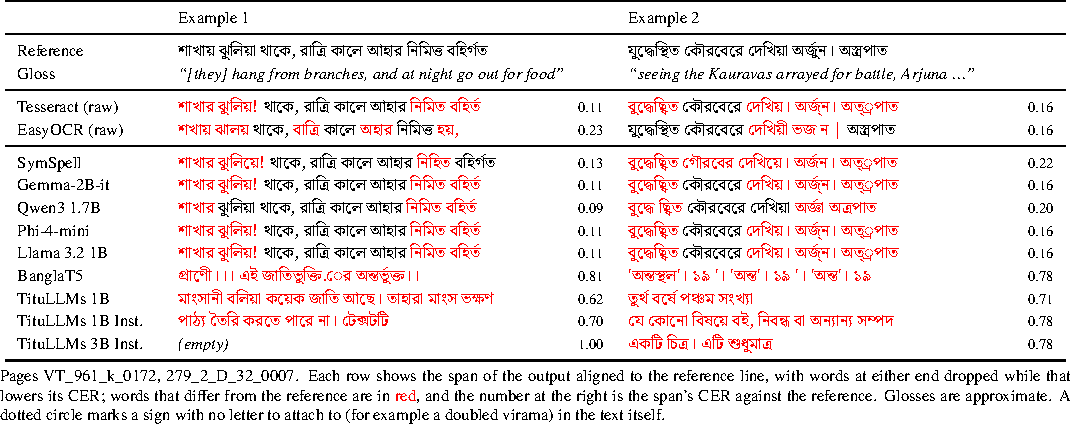
\includegraphics[width=\textwidth]{tables/examples_body.pdf}
\fi
\end{table*}
% ---- end tables/examples ----

\subsection{RQ3: Decoding, prompts and safeguards}
\label{sec:rq3}

\subsubsection{Decoding constraints}
\label{sec:decoding}
Table~\ref{tab:decoding} and Fig.~\ref{fig:decoding} compare plain greedy decoding with the repetition penalty alone, the four-gram ban alone and both together (guarded decoding), for the four general-purpose models on the 40 pages, with the OCR text of both engines and with the clean text as input. Every constraint, alone or combined, raised CER in all 33 completed comparisons with plain decoding (Phi-4-mini was not run on EasyOCR text), and all 33 increases are significant after Holm correction. Guarded decoding raised Gemma-2B-it's CER from 0.353 to 0.545 on Tesseract text, Qwen3 1.7B's from 0.337 to 0.925 and Phi-4-mini's from 0.354 to 1.740, so the three models that leave the OCR almost unchanged under plain decoding become clearly harmful. The clean-text control shows the same effect without any recognition error to repair: guarded decoding raised the CER of error-free input from 0.032 to 0.360 for Gemma-2B-it, from 0.035 to 0.940 for Qwen3 1.7B and from 0.060 to 1.406 for Phi-4-mini. The constrained outputs really are worse; what would mislead is to attribute that loss to the checkpoints' ability to correct, since the same checkpoints barely change their input under plain decoding. This comparison alone does not show why the constraints do this: besides acting on the prompt, a four-gram ban can block repetitions that the reference text itself contains, and a penalty can suppress valid repeated tokens. We therefore reran the four models on Tesseract and clean text with each constraint restricted to the generated tokens (Table~\ref{tab:decodinggen}). Restricting them removes much of the damage: the generated-only constraints are significantly less harmful than the whole-sequence ones in 21 of 24 settings, and with both constraints between 20\% and 91\% of the extra error disappears; Phi-4-mini's CER on Tesseract text falls from 1.740 to 0.688. Acting on the prompt is therefore a large part of the problem, but not all of it: the generated-only constraints are still significantly worse than plain decoding in 23 of 24 settings. The four-gram ban on the output alone adds 0.017 to 0.099 CER on Tesseract text, whereas the penalty on the output alone still adds 0.275 to 0.404 for Qwen3 1.7B, Phi-4-mini and Llama 3.2 1B (Gemma-2B-it: $+0.002$), so it also suppresses repetitions that the Bengali text genuinely contains. For copy-heavy correction, plain decoding is the safe choice.

% ---- begin tables/decoding_gen ----
\begin{table*}[t]
\centering
\caption{Repetition Constraints on the Whole Sequence and on Generated Tokens Only (Mean CER, 40 Pages)}
\label{tab:decodinggen}
\setlength{\tabcolsep}{4pt}
\footnotesize
\begin{tabular}{lcccccccc}
\toprule
 & & \multicolumn{2}{c}{Penalty} & \multicolumn{2}{c}{$n$-gram ban} & \multicolumn{2}{c}{Both (guarded)} & \\
\cmidrule(lr){3-4}\cmidrule(lr){5-6}\cmidrule(lr){7-8}
Model & Plain & Whole & Generated & Whole & Generated & Whole & Generated & \shortstack{Excess removed\\(both)} \\
\midrule
\multicolumn{9}{l}{\textit{Tesseract}} \\
Gemma-2B-it & 0.353 & 0.357 & 0.355$^{\circ}$ & 0.529 & 0.369$^{+}$ & 0.545 & 0.371$^{+}$ & 91\% \\
Qwen3 1.7B & 0.337 & 0.692 & 0.613$^{+}$ & 0.750 & 0.421$^{+}$ & 0.925 & 0.701$^{+}$ & 38\% \\
Phi-4-mini & 0.354 & 1.750 & 0.658$^{+}$ & 0.509 & 0.372$^{+}$ & 1.740 & 0.688$^{+}$ & 76\% \\
Llama 3.2 1B & 0.380 & 0.871 & 0.784$^{+\circ}$ & 0.795 & 0.479$^{+}$ & 0.972 & 0.785$^{+}$ & 32\% \\
\midrule
\multicolumn{9}{l}{\textit{Clean text}} \\
Gemma-2B-it & 0.032 & 0.049 & 0.045$^{+}$ & 0.327 & 0.117$^{+}$ & 0.360 & 0.103$^{+}$ & 78\% \\
Qwen3 1.7B & 0.035 & 0.628 & 0.454$^{+}$ & 0.625 & 0.191$^{+}$ & 0.940 & 0.537$^{+}$ & 45\% \\
Phi-4-mini & 0.060 & 1.282 & 0.280$^{+}$ & 0.366 & 0.080$^{+}$ & 1.406 & 0.327$^{+}$ & 80\% \\
Llama 3.2 1B & 0.119 & 0.812 & 0.775$^{+\circ}$ & 0.797 & 0.315$^{+}$ & 0.942 & 0.775$^{+}$ & 20\% \\
\bottomrule
\end{tabular}
\par\smallskip
\begin{minipage}{\linewidth}\footnotesize Whole: the constraint acts on the whole token sequence, prompt included, as \texttt{generate} applies it (Table~\ref{tab:decoding}); Generated: the same constraint restricted to the generated tokens (penalty 1.3 with \texttt{prompt\_ignore\_length}, four-gram ban on the output only). $^{+}$: significantly higher than plain decoding (23 of 24); $^{\circ}$: not significantly lower than the whole-sequence constraint (21 of 24 are lower). Wilcoxon signed-rank, Holm-corrected within each comparison type over the 24 settings (exploratory). Excess removed: the share of guarded decoding's increase over plain decoding that disappears when the constraints act on generated tokens only.\end{minipage}
\end{table*}
% ---- end tables/decoding_gen ----

Which constraint does the damage depends on the model. For Gemma-2B-it almost all of it comes from the $n$-gram ban ($+0.176$ on Tesseract text, against $+0.004$ for the penalty). For Phi-4-mini the penalty alone is catastrophic ($+1.396$, with 28 of 40 pages reaching the token limit) and the $n$-gram ban moderate ($+0.155$). For Qwen3 1.7B and Llama 3.2 1B each constraint alone raises CER by 0.35 to 0.49 on OCR text and by 0.59 to 0.69 on clean text. An evaluation that uses either constraint would thus misjudge a copying model, and testing only one of them would not show the size of the problem for every model. An earlier guarded-versus-plain comparison on the 15-page CPU sample (table note) also included two Bengali-pretrained checkpoints: guarded decoding raised the CER of the decoder-only TituLLMs 1B by more than 1, but not that of BanglaT5, an encoder-decoder model whose decoder does not see the input tokens as its own history.

\begin{figure*}[t]
\centering
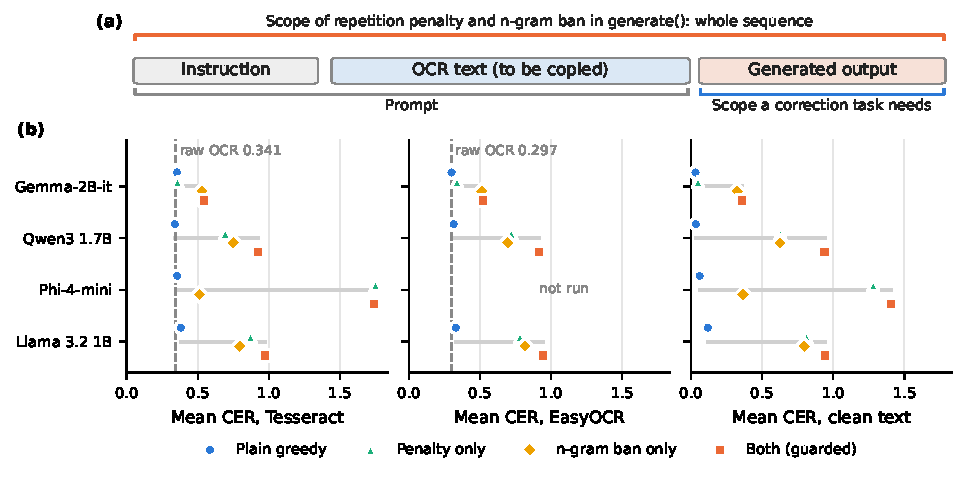
\includegraphics[width=0.85\textwidth]{figures/fig_decoding.pdf}
\caption{The decoding pitfall. (a) In the Transformers \texttt{generate} function, the repetition penalty and the $n$-gram ban act on the whole token sequence, which for a decoder-only model includes the OCR text in the prompt. (b) Mean CER of the four general-purpose models on the 40 pages under plain greedy decoding, the repetition penalty alone (1.3), the four-gram ban alone, and both (guarded), on Tesseract, EasyOCR and clean-text input; the dashed line is the raw OCR. Markers are offset vertically so that coinciding values stay visible.}
\label{fig:decoding}
\end{figure*}

% ---- begin tables/decoding ----
\begin{table*}[t]
\centering
\caption{Decoding Ablation on the 40 Pages: Repetition Penalty and $n$-Gram Ban, Alone and Together (Mean CER)}
\label{tab:decoding}
\setlength{\tabcolsep}{4pt}
\footnotesize
\begin{tabular}{llcccccll}
\toprule
Input & Model & Raw OCR & Plain & Penalty only & $n$-gram ban only & Both (guarded) & Guarded $-$ plain [95\% CI] & Truncated \\
\midrule
Tesseract & Gemma-2B-it & 0.341 & 0.353 & 0.357$^{+}$ & 0.529$^{+}$ & 0.545$^{+}$ & +0.192 [+0.156, +0.230] & 0/0/0 \\
Tesseract & Qwen3 1.7B & 0.341 & 0.337 & 0.692$^{+}$ & 0.750$^{+}$ & 0.925$^{+}$ & +0.587 [+0.532, +0.639] & 8/3/11 \\
Tesseract & Phi-4-mini & 0.341 & 0.354 & 1.750$^{+}$ & 0.509$^{+}$ & 1.740$^{+}$ & +1.385 [+1.175, +1.606] & 28/1/24 \\
Tesseract & Llama 3.2 1B & 0.341 & 0.380 & 0.871$^{+}$ & 0.795$^{+}$ & 0.972$^{+}$ & +0.592 [+0.508, +0.686] & 27/12/27 \\
\midrule
EasyOCR & Gemma-2B-it & 0.297 & 0.301 & 0.338$^{+}$ & 0.512$^{+}$ & 0.520$^{+}$ & +0.220 [+0.187, +0.257] & 0/0/0 \\
EasyOCR & Qwen3 1.7B & 0.297 & 0.315 & 0.721$^{+}$ & 0.695$^{+}$ & 0.917$^{+}$ & +0.602 [+0.548, +0.653] & 14/3/15 \\
EasyOCR & Llama 3.2 1B & 0.297 & 0.330 & 0.783$^{+}$ & 0.818$^{+}$ & 0.942$^{+}$ & +0.612 [+0.529, +0.700] & 21/21/23 \\
\midrule
Clean text & Gemma-2B-it & -- & 0.032 & 0.049$^{+}$ & 0.327$^{+}$ & 0.360$^{+}$ & +0.328 [+0.298, +0.359] & 0/0/0 \\
Clean text & Qwen3 1.7B & -- & 0.035 & 0.628$^{+}$ & 0.625$^{+}$ & 0.940$^{+}$ & +0.905 [+0.850, +0.966] & 10/7/22 \\
Clean text & Phi-4-mini & -- & 0.060 & 1.282$^{+}$ & 0.366$^{+}$ & 1.406$^{+}$ & +1.345 [+1.093, +1.618] & 19/2/18 \\
Clean text & Llama 3.2 1B & -- & 0.119 & 0.812$^{+}$ & 0.797$^{+}$ & 0.942$^{+}$ & +0.824 [+0.766, +0.885] & 27/17/25 \\
\bottomrule
\end{tabular}
\par\smallskip
\begin{minipage}{\linewidth}\footnotesize Plain: greedy decoding with only the length cap (the main runs). Penalty: \texttt{repetition\_penalty}=1.3; $n$-gram ban: \texttt{no\_repeat\_ngram\_size}=4; in a decoder-only model both also act on the prompt, so they penalise copying the OCR text. Clean text: the reference given as input, so any change is damage. $^{+}$/$^{-}$: higher/lower than plain decoding, Wilcoxon signed-rank test, Holm-corrected over the 33 preset-versus-plain tests (exploratory family). CI: paired bootstrap, 10{,}000 resamples, seed 403. Truncated: pages that reached the token limit (penalty/$n$-gram/both), of 40. Phi-4-mini was not run on EasyOCR text (time limit of the GPU session). An earlier ablation of guarded against plain decoding on 15 pages (August OCR, CPU, bfloat16) also covered two Bengali-pretrained checkpoints; guarded minus plain CER on Tesseract and EasyOCR text: TituLLMs 1B +1.07 and +1.56; BanglaT5 -0.01 and -0.02.\end{minipage}
\end{table*}
% ---- end tables/decoding ----

\subsubsection{Prompt and chunking variants}
\label{sec:variants}
Table~\ref{tab:variants} reports the four general-purpose models under the three prompt variants and the model-independent chunks. No variant brings any model significantly below the raw OCR. The preserve-spelling instruction lowered mean CER in seven of the eight model-and-engine pairs, by up to 0.026 (Llama 3.2 1B on EasyOCR output), but none of these changes is significant. The Bengali prompt and the three worked examples raised CER in most pairs; the increase is significant for Llama 3.2 1B with the Bengali prompt on both engines and with the examples on Tesseract output, and for Phi-4-mini with the Bengali prompt on EasyOCR output. Chunks of at most 300 characters changed mean CER by at most 0.016, with no significant change.

% ---- begin tables/variants ----
\begin{table}[t]
\centering
\caption{Prompt and Chunking Variants (Mean CER, 40 Pages)}
\label{tab:variants}
\setlength{\tabcolsep}{4pt}
\footnotesize
\begin{tabular}{llcc}
\toprule
Model & Variant & Tesseract & EasyOCR \\
\midrule
 & Raw OCR & 0.341 & 0.297 \\
\midrule
Gemma-2B-it & original & 0.353 & 0.301 \\
 & preserve spelling & 0.350 & 0.305 \\
 & Bengali prompt & 0.359 & 0.326 \\
 & three-shot & 0.435 & 0.390 \\
 & 300-char chunks & 0.343 & 0.300 \\
\midrule
Qwen3 1.7B & original & 0.337 & 0.315 \\
 & preserve spelling & 0.335 & 0.310 \\
 & Bengali prompt & 0.390 & 0.308 \\
 & three-shot & 0.368 & 0.303 \\
 & 300-char chunks & 0.343 & 0.299 \\
\midrule
Phi-4-mini & original & 0.354 & 0.315 \\
 & preserve spelling & 0.351 & 0.312 \\
 & Bengali prompt & 0.402 & 0.359$^{*}$ \\
 & three-shot & 0.447 & 0.324 \\
 & 300-char chunks & 0.343 & 0.319 \\
\midrule
Llama 3.2 1B & original & 0.380 & 0.330 \\
 & preserve spelling & 0.362 & 0.304 \\
 & Bengali prompt & 0.516$^{*}$ & 0.459$^{*}$ \\
 & three-shot & 0.480$^{*}$ & 0.395 \\
 & 300-char chunks & 0.380 & 0.321 \\
\bottomrule
\end{tabular}
\par\smallskip
\begin{minipage}{\linewidth}\footnotesize Original: English prompt, chunks of about 250 tokens. Each variant changes one thing: the preserve-spelling instruction, the prompt in Bengali, three worked examples, or chunks of at most 300 characters. $^{*}$: differs from the original setting, two-sided Wilcoxon signed-rank test, Holm-corrected over the 32 variant comparisons (exploratory family). Equal entries in a column come from different outputs (unrounded: Tesseract: Gemma-2B-it 300-char chunks 0.3432, Qwen3 1.7B 300-char chunks 0.3434, Phi-4-mini 300-char chunks 0.3435; Tesseract: Llama 3.2 1B original 0.3799, Llama 3.2 1B 300-char chunks 0.3796; EasyOCR: Qwen3 1.7B original 0.3146, Phi-4-mini original 0.3147).\end{minipage}
\end{table}
% ---- end tables/variants ----

Two checks of prompt fit change no conclusion (appendix). The instruction-tuned TituLLMs checkpoints often answer with commentary; a generous commentary filter (Table~\ref{tab:filter}) lowers the CER of TituLLMs 1B Instruct on Tesseract text from 1.64 to 0.87, but every Bengali-pretrained checkpoint stays far above the raw OCR (0.87 to 0.98 against 0.341), and the general-purpose models change by at most 0.009. Float32 precision and a completion-style prompt likewise leave every Bengali-pretrained checkpoint significantly worse than the raw OCR (Table~\ref{tab:checks}).

\subsubsection{Confidence gating}
\label{sec:gating}
Confidence gating (Table~\ref{tab:gated}) works at the word level instead of the page level. The engines are unsure of much of the text: 41\% of Tesseract words have a confidence below 50 and 77\% below 90, and 52\% of EasyOCR words lie in boxes below 0.5. Gating reduces the damage of the harmful methods, for example lowering the CER of TituLLMs 1B on Tesseract output from 1.084 to 0.454 and that of the dictionary baseline from 0.378 to 0.348 at the lowest threshold, but nearly all of them remain significantly worse than the raw OCR. For the general-purpose models gating keeps the CER at or just below the raw OCR on Tesseract output. Qwen3 1.7B at threshold 70 gives the only significant reduction of CER in this study (engine fusion gains about as much, but not significantly; Section~\ref{sec:classical}), from 0.341 to 0.337 ($-0.004$, 95\% CI $[-0.006,-0.002]$, $p=0.038$ after Holm correction over 54 tests), 1.1\% of the raw CER. Gating left 4 of the 40 pages identical to the raw OCR; of the 36 non-zero differences the test uses, 25 are improvements and 11 deteriorations. The gain is negligible and not robust: after Holm correction it is not significant at thresholds 50 or 90 (unadjusted $p=0.014$ and 0.069), not on EasyOCR output, and the ungated Qwen3 change it starts from is itself not significant. On EasyOCR output, where confidence is per box and therefore coarse, no gated method improves on the raw OCR. The thresholds were fixed in advance, not chosen on these pages, but the development pages have no confidence scores from this OCR run, so the gain could not be validated on held-out pages; we report it as exploratory. Lower thresholds, which allow fewer changes, give the lowest error throughout.

% ---- begin tables/gated ----
\begin{table}[t]
\centering
\caption{Confidence-Gated Correction (Mean CER, 40 Pages)}
\label{tab:gated}
\setlength{\tabcolsep}{2pt}
\footnotesize
\begin{tabular}{lcccccc}
\toprule
 & \multicolumn{3}{c}{Tesseract (word conf.)} & \multicolumn{3}{c}{EasyOCR (box conf.)} \\
\cmidrule(lr){2-4}\cmidrule(lr){5-7}
Method & 50 & 70 & 90 & 0.5 & 0.7 & 0.9 \\
\midrule
Raw OCR & 0.341 & 0.341 & 0.341 & 0.297 & 0.297 & 0.297 \\
\midrule
SymSpell (dictionary) & 0.348$^{+}$ & 0.353$^{+}$ & 0.365$^{+}$ & 0.315$^{+}$ & 0.328$^{+}$ & 0.334$^{+}$ \\
Gemma-2B-it & 0.340 & 0.340 & 0.341 & 0.298 & 0.300 & 0.302 \\
Qwen3 1.7B & 0.338 & 0.337$^{-}$ & 0.338 & 0.297 & 0.305 & 0.306 \\
Phi-4-mini & 0.338 & 0.338 & 0.340 & 0.297 & 0.301 & 0.308 \\
Llama 3.2 1B & 0.342 & 0.348 & 0.356 & 0.303 & 0.318$^{+}$ & 0.325$^{+}$ \\
BanglaT5 & 0.440$^{+}$ & 0.441$^{+}$ & 0.480$^{+}$ & 0.375$^{+}$ & 0.450$^{+}$ & 0.569$^{+}$ \\
TituLLMs 1B & 0.454$^{+}$ & 0.511$^{+}$ & 0.619$^{+}$ & 0.444$^{+}$ & 0.674$^{+}$ & 0.868$^{+}$ \\
TituLLMs 1B Instruct & 0.427$^{+}$ & 0.541$^{+}$ & 0.813$^{+}$ & 0.567$^{+}$ & 0.834$^{+}$ & 1.061$^{+}$ \\
TituLLMs 3B Instruct & 0.357 & 0.346 & 0.365 & 0.317 & 0.382 & 0.519$^{+}$ \\
\bottomrule
\end{tabular}
\par\smallskip
\begin{minipage}{\linewidth}\footnotesize A model's edit is kept only where every OCR word it changes has a confidence below the threshold (column header); elsewhere the raw OCR is kept. $^{+}$/$^{-}$: significantly higher/lower than the raw OCR, Wilcoxon signed-rank test, Holm-corrected over the 54 gated tests (exploratory family); pages left identical to the raw OCR are dropped by the test.\end{minipage}
\end{table}
% ---- end tables/gated ----

% =====================================================================
\section{Discussion}
\label{sec:discussion}

For practice, a correction step has to improve on keeping the raw OCR. We answer the three research questions, then discuss why word-level gains come without character-level gains, what explains the failures, and what follows for institutions.

\subsection{Answers to the research questions}
\textbf{RQ1.} At the character level, not under the evaluated conditions. No ungated model significantly reduced mean code-point CER, bounded cMER or pooled CER on either engine (Tables~\ref{tab:matrix}, \ref{tab:robustness} and~\ref{tab:scale}), nor on region-level OCR (Table~\ref{tab:region}); the 10-page intervals of Qwen3 32B include zero (Table~\ref{tab:large}). On the grapheme-cluster CER, Qwen3 1.7B on Tesseract text is the one significant exception (Section~\ref{sec:main}). The word error rate behaves differently: Qwen3 1.7B on Tesseract text, Qwen3 4B and 8B and the fine-tuned ByT5-small on both engines, and Llama 3.2 3B on EasyOCR text lower it significantly, as do Qwen3 4B on EasyOCR region text and two models at the highest synthetic noise level. The only significant CER reduction is exploratory and small, about 1\% of the raw CER: Qwen3 1.7B with confidence gating at one of three thresholds (Table~\ref{tab:gated}). Engine fusion gains about as much, but we report this gain as descriptive, not significant (Table~\ref{tab:classical}). The engines and the two OCR settings agree in direction and ranking.

\textbf{RQ2.} Preservation is the larger problem. Every method changed error-free text (Tables~\ref{tab:clean}, \ref{tab:scale} and~\ref{tab:finetune}), from CER 0.015 for the fine-tuned model to more than 0.8 for the Bengali-pretrained checkpoints, which regenerate the text and lose most correct words. The general-purpose core models keep most of their input, and the attribution maps on sampled chunks are consistent with copying (Table~\ref{tab:attribution}, appendix); they repair few words, and only Qwen3 1.7B on Tesseract text repairs more than it breaks. The larger Qwen3 models and the fine-tuned model repair more words than they break, but their other edits add at least as many character errors as the repairs remove (Table~\ref{tab:editlevel}).

\textbf{RQ3.} Repetition constraints that include the prompt changed the outcome most: alone or together they made every general-purpose model significantly worse, on OCR text and on error-free text (Table~\ref{tab:decoding}). Restricted to generated tokens they did much less damage, but still significantly more than plain decoding in all but one setting (Table~\ref{tab:decodinggen}). Float32 precision and a completion prompt did not bring a Bengali-pretrained checkpoint near the raw OCR (Table~\ref{tab:checks}). No tested prompt variant, chunking scheme or page-level safeguard produced a statistically significant CER reduction relative to raw OCR (Tables~\ref{tab:variants} and~\ref{tab:safeguards}), although some lowered mean CER slightly (for example 0.335 against 0.341 for Qwen3 1.7B with the preserve-spelling instruction on Tesseract text). Confidence gating and engine fusion reduced the damage, with the small gains noted under RQ1.

Table~\ref{tab:claims} lists each main claim with its evidence and states whether it rests on the primary test family, an exploratory test or a descriptive analysis.

% ---- begin tables/claims ----
% Claim-to-evidence summary (external review 2026-10-19, item 12). Hand-written
% design table: claims, where the evidence is, and its status; no numbers.
\begin{table*}[t]
\centering
\caption{Main Claims, Their Evidence and Their Status}
\label{tab:claims}
\setlength{\tabcolsep}{3.5pt}
\footnotesize
\renewcommand{\arraystretch}{1.12}
\begin{tabular}{>{\raggedright\arraybackslash}p{7.4cm}>{\raggedright\arraybackslash}p{4.6cm}>{\raggedright\arraybackslash}p{5.2cm}}
\toprule
Claim & Evidence & Status \\
\midrule
No ungated model significantly lowers code-point CER on whole-page OCR & Table~\ref{tab:matrix}; Tables~\ref{tab:robustness}, \ref{tab:scale}, \ref{tab:large} & Primary family (eight core models, dictionary); exploratory for the other models and measures \\
The same holds for region-level OCR and for synthetic noise down to an input CER of 0.02 & Tables~\ref{tab:region}, \ref{tab:noise} & Exploratory, Holm within each family \\
Larger Qwen3 models and the fine-tuning pilot lower WER but not CER & Tables~\ref{tab:scale}, \ref{tab:finetune} & Exploratory; the pilot is under-trained \\
Their word repairs are offset by edits to other words & Table~\ref{tab:editlevel} & Descriptive \\
Every method changes error-free text & Tables~\ref{tab:clean}, \ref{tab:scale}, \ref{tab:finetune} & Descriptive stress test of preservation \\
Repetition constraints make copying models much worse & Table~\ref{tab:decoding} & Exploratory, Holm within the family \\
In Transformers~5.19.0 these constraints also act on the prompt & One-step test, Section~\ref{sec:correction} & Verified \\
Restricting them to generated tokens removes much, but not all, of the damage & Table~\ref{tab:decodinggen} & Exploratory, Holm within each comparison \\
Confidence gating gives a small CER gain at one of three thresholds & Table~\ref{tab:gated} & Exploratory, not validated on held-out pages \\
Engine fusion gains about as much & Table~\ref{tab:classical} & Descriptive (test family chosen after a first scoring) \\
The tested Bengali-pretrained checkpoints regenerate text instead of editing it & Tables~\ref{tab:matrix}, \ref{tab:diagnostics}, \ref{tab:filter}; Fig.~\ref{fig:corrected} & Descriptive; specific to these checkpoints and prompts \\
\bottomrule
\end{tabular}
\end{table*}
% ---- end tables/claims ----

\subsection{Word-level gains without character-level gains}
A word counts as fixed only when it becomes exactly right, and as broken when any of its characters changes; CER also counts every changed character inside words that stay wrong, and every insertion and deletion. A model can therefore turn more words right than wrong, as the larger Qwen3 models and the fine-tuned model do, without lowering CER. The edit-level analysis (Section~\ref{sec:editlevel}) shows what offsets the repairs: the repaired words were mostly one sign away from correct, while the same models also change consonants in words that stay wrong and break some correct words, which together add at least as many character errors as the repairs remove. The distinction matters for use: a collection searched by whole words might benefit from the word-level gains, whereas a faithful transcription needs the character-level result. We did not measure either downstream use.

\subsection{Relation to prior work}
Our outcome agrees with reported zero-shot failures on Finnish~\cite{kanerva2025nofreelunches}, on historical transcripts in several languages~\cite{boros2024postcorrection} and on Hindi speech-recognition output~\cite{kumar2026postasr}, and our clean-text control measures directly the over-correction that HIPE-OCRepair~\cite{ehrmann2026hipeocrepair} and a study of GPT models on historical English~\cite{zhang2024prosody} report. The successful studies fine-tune for correction~\cite{thomas2024leveraging,ehrmann2026hipeocrepair}, use a frontier model~\cite{viana2026reframing}, or start from nearly clean English~\cite{koynov2025opportunities}. Our input CER (0.30 to 0.34) exceeds the 0.25 or less of those studies, but high input CER alone does not account for the difference: a 70-billion-parameter model helped at an input CER of 0.07~\cite{koynov2025opportunities}, whereas the small models here made even synthetic text with a CER of 0.02 worse, and they did not help on region-level OCR (0.23 and 0.33) either. The decoding ablation adds a caution for negative results in general: before a failure is attributed to correction itself, it should be checked under plain decoding.

\subsection{Possible explanations}
\begin{itemize}
\item \emph{Input noise.} High input CER alone does not explain the failures: every method damaged error-free text, every general-purpose model raised CER at all five synthetic noise levels down to 0.020 (Section~\ref{sec:noise}), and region-level OCR, with a lower input CER, was made worse more consistently than whole-page OCR (Section~\ref{sec:region}). The structure of real OCR errors, historical vocabulary or interactions between error types may still matter; the synthetic noise only approximates real errors, which the models handle somewhat better at the same CER.
\item \emph{Model size.} Within Qwen3, size moves correction towards repairing words: from 0.6B to 8B the balance of fixed and broken words turns from negative to positive, and WER falls. CER does not fall, and at 32B the model changes error-free text more than the smaller Qwen3 models (Section~\ref{sec:scale}). Up to 32 billion parameters in 4-bit, size alone did not make zero-shot correction lower CER.
\item \emph{Task-specific training.} A briefly trained pilot learned to copy and edit: it changed error-free text least of all methods and lowered WER, but not CER (Section~\ref{sec:finetune}). Because it saw only a third of its training data once, it does not show whether full training would lower CER.
\item \emph{Tokenisation.} Bengali needs several times the token count of English under English-centric tokenizers~\cite{petrov2023tokenizer,ahia2023cost}, and our models use 0.29 to 1.22 tokens per character (Table~\ref{tab:cost}). Fertility does not rank the outcomes: Llama 3.2 1B and TituLLMs 1B share a tokenizer and the highest fertility, yet one stays near the baseline while the other triples its error rate.
\item \emph{Historical spelling.} A model or lexicon built for modern Bengali may mistake older spellings for errors. Our subtitle dictionary replaces about 31 correct words per page of clean text, and half of the reference words are missing from it. A Wikipedia lexicon, which misses about a third of them, together with a smaller edit distance, cuts the dictionary's damage by four-fifths but does not remove it (Section~\ref{sec:classical}). Asking models to preserve spelling slightly reduces damage in seven of the eight general-purpose model-and-engine pairs. Mixing old and modern literary registers also caused difficulty for GPT-4o in grammar correction~\cite{bhattacharyya2025banglagec}. Historical spelling is therefore part of the explanation for the dictionary; for the language models we have not tested its effect directly.
\item \emph{Prompt format and instruction-following.} The instruction-tuned TituLLMs checkpoints often describe the input or return nothing rather than correct it. The prompt format explains only part of this: a completion prompt lowered the base checkpoint's CER by about 0.2 but left it far above the raw OCR, and normalising BanglaT5's input changed nothing (Section~\ref{sec:precision}). Instruction tuning that did not cover copy-and-edit tasks is a plausible cause; with a completion prompt instead of their template, TituLLMs 1B Instruct improved (CER 1.642 to 1.336 on Tesseract text) and 3B Instruct did not (0.958 to 0.960), and both stayed far worse than the raw OCR.
\end{itemize}
These explanations and results apply to the checkpoints and configuration tested here. They do not establish how other Bengali-pretrained checkpoints, or models fine-tuned with more data or with real OCR pairs, would perform.

\subsection{Practical implications}
For comparable historical Bengali material, the evidence supports keeping the raw OCR and validating any correction step against reference transcriptions before it replaces the OCR text. Keeping the raw OCR also saves two to fourteen minutes of CPU time per page, as measured on the 15-page sample (Table~\ref{tab:cost}). Restricting edits to low-confidence words reduced the damage of every method that had increased error, and fusing two engines by word confidence needs no model and no GPU and broke the fewest correct words; both gained about 1\% of the raw CER at best, in exploratory tests that need validation on held-out material. Larger models and the fine-tuned model lowered WER but not CER, so a project that values whole-word accuracy, for example for search, might consider them after checking their damage to correct text; we did not measure search or other downstream uses. In copy-heavy correction with Transformers generation, leave repetition constraints off: restricting them to generated tokens reduced their damage but did not remove it.
\subsection{Threats to validity and limitations}
\begin{itemize}
\item \emph{Sample size and statistics.} With 40 pages from 37 books the intervals are moderately wide. Only the 36 CER and WER tests of the main evaluation form the primary family; every other test is exploratory, Holm correction holds only within each family, and the 10-page comparison of the 32-billion-parameter model cannot reach significance at all.
\item \emph{Reference coverage and order.} The engines read the whole page, while the ground truth covers the annotated regions in file order. A reference in the declared reading order, an order-free word recall and region-level OCR gave the same conclusions, but the region-level Tesseract text comes from a later build whose output differs from the main run, so it is compared only with whole-page text of that build and never mixed with the main run's text.
\item \emph{Reuse of data.} The few-shot examples, the noise model and the fine-tuning checkpoint come from the 10 development pages, which were also used for debugging. The extensions were added after the main evaluation and reuse its 40 pages; the region crop settings were compared on 8 of them, and the fusion test family was fixed after a first scoring. The guarded decoding setting was chosen after seeing development output.
\item \emph{Model and prompt fit.} The results describe the tested checkpoint and prompt combinations: the instruction-tuned TituLLMs checkpoints received their shipped template and, on Tesseract text only, a completion prompt; no output filter removed preambles (which penalises the TituLLMs Instruct checkpoints most; the copying models add almost none), and Phi-4-mini was rerun in float32 on Tesseract text only.
\item \emph{Environment.} PyTorch and CUDA versions of the main runs were not recorded, and the OCR could not be regenerated a week later; the released outputs, not a rerun, are the reference for every reported score.
\item \emph{Metric scope.} We measured string agreement with the reference, not search, information extraction or a human corrector's time. WER and CER can disagree, as they do for the larger models.
\item \emph{External validity.} The pages are early printed books from one release, chosen by whether a transcription exists and labelled by page type by one annotator, so the page-type figures are descriptive; the results may not transfer to modern print or other collections. They also cover only the tested sizes: up to 8 billion parameters on 40 pages and one 32-billion-parameter model on 10, so they say nothing about frontier-scale models.
\end{itemize}
Three extensions follow most directly from these findings. First, the small gating and fusion gains were found in exploratory tests and need validation on held-out pages. Second, the fine-tuning pilot should be repeated with a complete training schedule, more data, or real OCR pairs once they exist, before anything is concluded about task-specific training. Third, because WER and CER diverge, the value of correction for search, extraction or a human corrector should be measured directly. Other collections, larger models and multimodal transcription would widen the scope.

% =====================================================================
\section{Conclusion}

We evaluated small language models as a post-correction step for historical Bengali OCR. On 40 pages of historical printed Bengali from one collection, read by two engines, none of the ungated models significantly reduced mean code-point CER, on whole pages, on region-level OCR or on synthetic noise down to an input CER of 0.02. Larger Qwen3 models and a briefly trained fine-tuning pilot repaired more words than they broke and lowered the word error rate, but their edits to other words added at least as many character errors as the repairs removed. Every method changed error-free text, and repetition constraints that included the source prompt substantially worsened the outputs of models that otherwise copy their input. Confidence gating and engine fusion reduced the damage but gained only about 1\% of the raw CER, in exploratory tests. For comparable material, institutions should keep the raw OCR and validate any correction step on reference transcriptions before it replaces the OCR text. These findings do not establish the limits of task-specific training, performance on other Bengali collections, or the value of correction for search and other downstream uses.

\appendices
\section{Additional Results}
This appendix holds the secondary diagnostics: the per-page analysis, the precision and prompt-format checks with the commentary filter, the edit profiles, the gradient-based attribution, the page-level safeguards, a check of CPU against GPU runs, and further tables.

\subsection{Per-page analysis}
Figure~\ref{fig:corrected} plots each page's corrected CER against its baseline CER, and Fig.~\ref{fig:scatter} the change in CER against the baseline CER. Two patterns appear. For the general-purpose models and the dictionary baseline, the points lie along the identity line and corrected CER follows baseline CER almost exactly (Spearman $\rho$ between 0.88 and 1.00 on both engines): these methods leave most of each page as it was, so the page's own difficulty determines its score. Qwen3 1.7B lowered CER on 22 of the 40 Tesseract pages and Gemma-2B-it on 16, but by amounts that their increases on other pages offset. For BanglaT5 and the TituLLMs models, corrected CER is unrelated or only weakly related to baseline CER ($\rho$ between $-0.00$ and 0.55): their output has a similar error rate whatever the input quality, which suggests that they regenerate the text instead of editing it. Their points form a horizontal band above the identity line (Fig.~\ref{fig:corrected}; the change in CER is plotted in Fig.~\ref{fig:scatter}). Split into thirds by baseline CER, BanglaT5, TituLLMs 1B and TituLLMs 3B Instruct have their smallest increase on the hardest third on both engines (TituLLMs 3B Instruct on Tesseract output: $+0.85$ on the easiest third, $+0.39$ on the hardest), and the dictionary shows the same pattern on a smaller scale; the general-purpose models stay within 0.07 of zero in every third.

\begin{figure*}[t]
\centering
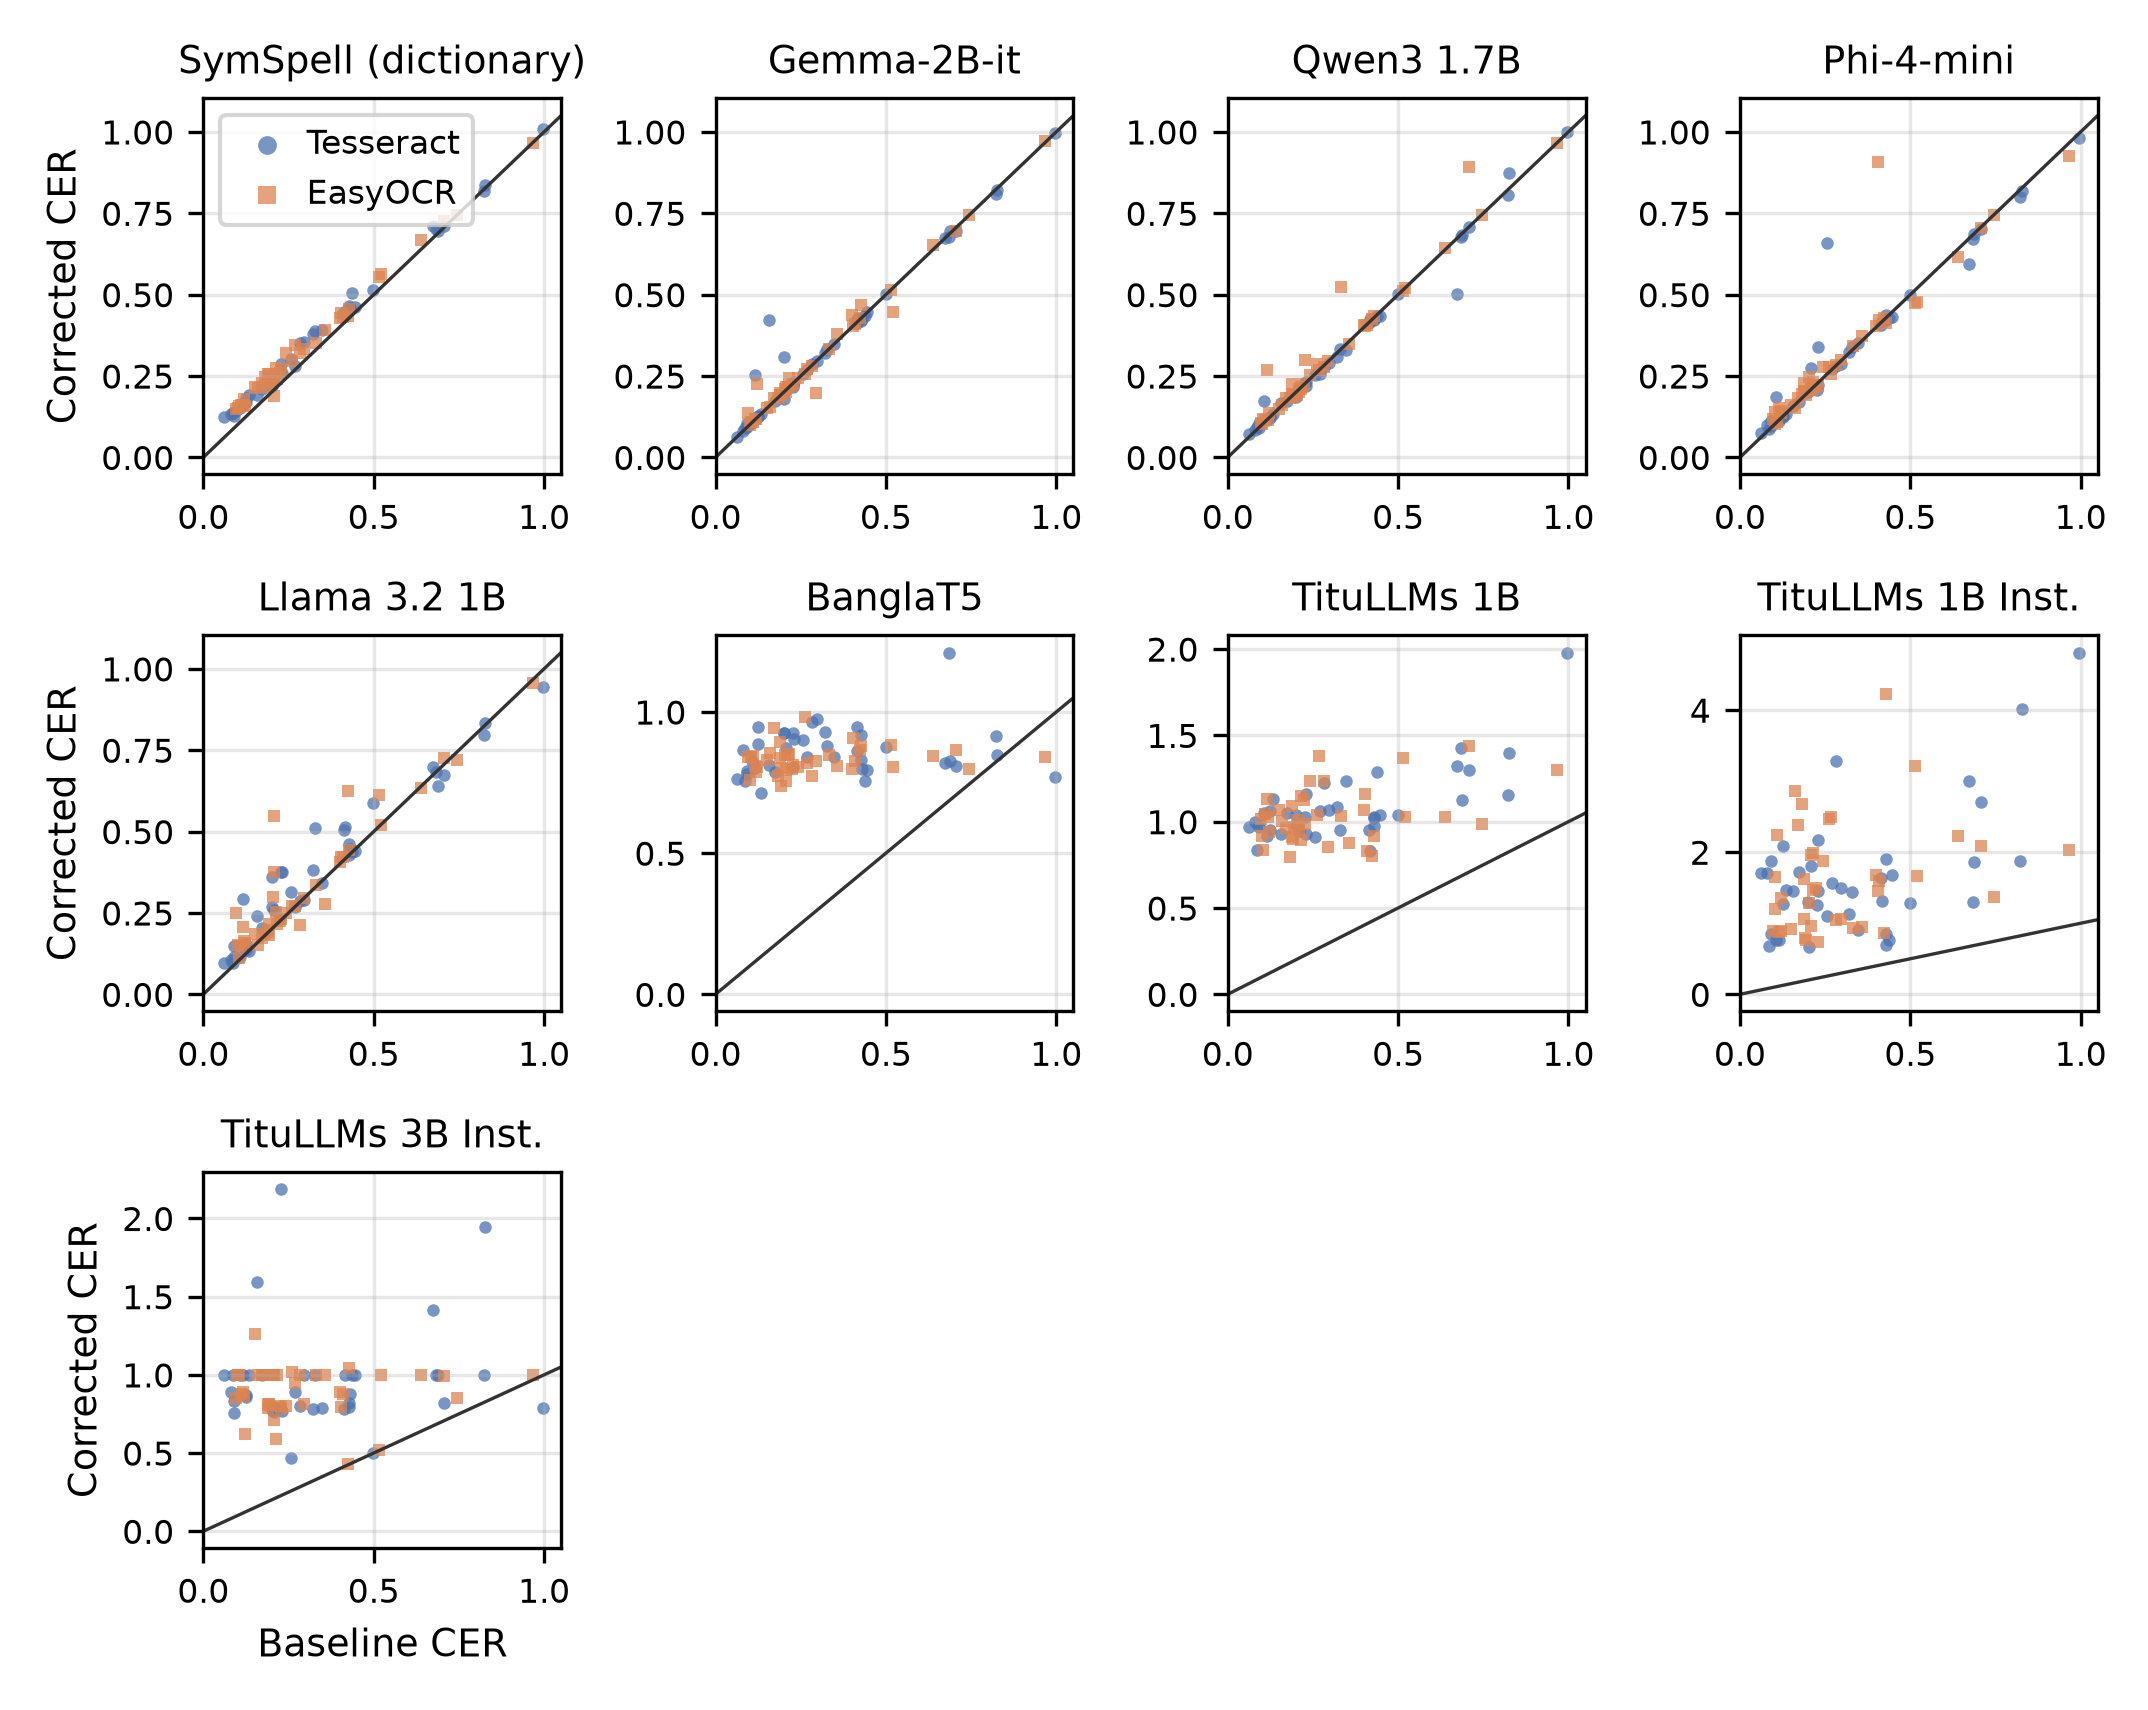
\includegraphics[width=\textwidth]{figures/fig_corrected.png}
\caption{Corrected CER per page against the page's baseline CER, one panel per method, for Tesseract (circles) and EasyOCR (squares). The diagonal is the identity line: points on it have the same CER as the raw OCR, points below it a lower CER. Vertical scales differ between panels.}
\label{fig:corrected}
\end{figure*}


\subsection{Precision and prompt format}
\label{sec:precision}
Two choices in the main runs could have made the Bengali-pretrained checkpoints look worse than they are: the numerical precision of the two largest models, and the prompt format (Table~\ref{tab:checks}).

\textbf{Precision.} TituLLMs 3B Instruct, run in float16, returned an empty page in 43 of its 120 outputs, each within 0.2 to 0.5~s, so it ended generation at or near its first token. Float16 overflow could cause this, so we reran it in float32 and recorded its first-token logits in both precisions. The first token was the same on all 208 chunks, and the end-of-sequence token on the same 87; no value was infinite or NaN, and the largest activation, about 1{,}000, was far below the float16 limit of 65{,}504. The float32 run returned the same empty pages and changed mean CER by at most 0.002 on OCR text and by $-0.040$ on the clean text, not significantly (95\% CI $[-0.132,+0.032]$), and Phi-4-mini in float32 gave the same CER on Tesseract text (0.354). The empty pages are the model's own behaviour, not a precision artefact.

\textbf{Prompt format.} The base TituLLMs 1B checkpoint received our instruction as plain text with no cue for where its answer should begin. With a completion-style prompt that ends with such a cue, its CER fell from 1.084 to 0.877 on Tesseract text, from 1.033 to 0.861 on EasyOCR text and from 0.988 to 0.605 on the clean text (Wilcoxon signed-rank, unadjusted $p<0.001$ in each case; exploratory), but it remains far worse than the raw OCR ($+0.54$ and $+0.56$ CER on OCR text). Passing BanglaT5's input through the normaliser its model card asks for changed its CER by at most 0.002. The prompt format thus matters for the base checkpoint, but neither check changes a conclusion: every rerun of a Bengali-pretrained checkpoint stays significantly worse than the raw OCR.

% ---- begin tables/checks ----
\begin{table*}[t]
\centering
\caption{Precision and Prompt-Format Checks (Mean CER, 40 Pages)}
\label{tab:checks}
\setlength{\tabcolsep}{3pt}
\scriptsize
\begin{tabular}{llcccccc}
\toprule
 & & \multicolumn{2}{c}{Tesseract} & \multicolumn{2}{c}{EasyOCR} & \multicolumn{2}{c}{Clean text} \\
\cmidrule(lr){3-4}\cmidrule(lr){5-6}\cmidrule(lr){7-8}
Check & Model & Main / check & $\Delta$ [95\% CI] & Main / check & $\Delta$ [95\% CI] & Main / check & $\Delta$ [95\% CI] \\
\midrule
Float32 & TituLLMs 3B Instruct & 0.958 / 0.959 & +0.000 [-0.001, +0.001] & 0.886 / 0.888 & +0.002 [-0.000, +0.005] & 0.967 / 0.927 & -0.040 [-0.132, +0.032] \\
Float32 & Phi-4-mini & 0.354 / 0.354 & -0.000 [-0.001, +0.000] & -- & -- & -- & -- \\
Completion prompt & TituLLMs 1B & 1.084 / 0.877 & -0.206$^{*}$ [-0.276, -0.118] & 1.033 / 0.861 & -0.172$^{*}$ [-0.262, -0.055] & 0.988 / 0.605 & -0.383$^{*}$ [-0.488, -0.295] \\
Normalised input & BanglaT5 & 0.860 / 0.858 & -0.001 [-0.014, +0.013] & 0.831 / 0.830 & -0.001 [-0.004, +0.002] & 0.833 / 0.831 & -0.002 [-0.007, +0.004] \\
\bottomrule
\end{tabular}
\par\smallskip
\begin{minipage}{\linewidth}\footnotesize Float32: instead of float16. Main: the setting of the main runs (float16 for the two models above 3B parameters; each model's shipped chat template; BanglaT5 on unnormalised text). Check: the same model rerun with one change. $\Delta$: check $-$ main; CI: paired bootstrap, 10{,}000 resamples; $^{*}$: Wilcoxon signed-rank $p<0.05$, unadjusted (exploratory); the three completion-prompt changes have $p<0.001$. --: Phi-4-mini in float32 was not run on EasyOCR text, and on the clean text only 1 of 40 pages finished within the session's time limit, so neither is reported. Float32 reruns: two Kaggle T4 GPUs. First-token check of TituLLMs 3B Instruct on all 208 chunks: the same first token in both precisions on 208, end-of-sequence first on 87 in both, no non-finite logits or hidden states, largest activation 1000 (float16 limit 65{,}504). Empty pages (float16/float32, Tesseract, EasyOCR, clean text): 13/13, 14/14, 16/16. Every check of a Bengali-pretrained checkpoint stays significantly worse than the raw OCR ($+$0.52 to $+$0.62 CER on OCR text, $p<0.001$).\end{minipage}
\end{table*}
% ---- end tables/checks ----

% ---- begin tables/filter ----
\begin{table*}[t]
\centering
\caption{Mean CER With a Generous Commentary Filter (40 Pages)}
\label{tab:filter}
\setlength{\tabcolsep}{5pt}
\footnotesize
\begin{tabular}{lcccccc}
\toprule
 & \multicolumn{3}{c}{Tesseract (raw 0.341)} & \multicolumn{3}{c}{EasyOCR (raw 0.297)} \\
\cmidrule(lr){2-4}\cmidrule(lr){5-7}
Model & Output & Filtered & Lines dropped & Output & Filtered & Lines dropped \\
\midrule
Gemma-2B-it & 0.353 & 0.348 & 15 / 890 & 0.301 & 0.299 & 19 / 1876 \\
Qwen3 1.7B & 0.337 & 0.337 & 1 / 764 & 0.315 & 0.316 & 37 / 1423 \\
Phi-4-mini & 0.354 & 0.345 & 6 / 797 & 0.315 & 0.306 & 25 / 1525 \\
Llama 3.2 1B & 0.380 & 0.379 & 2 / 829 & 0.330 & 0.329 & 10 / 1813 \\
BanglaT5 & 0.860 & 0.940 & 43 / 62 & 0.831 & 0.968 & 50 / 63 \\
TituLLMs 1B & 1.084 & 0.895 & 61 / 616 & 1.033 & 0.882 & 210 / 2001 \\
TituLLMs 1B Instruct & 1.642 & 0.866 & 339 / 840 & 1.633 & 0.901 & 461 / 1636 \\
TituLLMs 3B Instruct & 0.958 & 0.976 & 41 / 147 & 0.886 & 0.942 & 70 / 256 \\
\bottomrule
\end{tabular}
\par\smallskip
\begin{minipage}{\linewidth}\footnotesize Filter: an output line is dropped when fewer than 30\% of its character trigrams occur in the page's OCR input. It removes preambles and descriptions of the text, but also invented lines, so the filtered CER is a lower bound for any such filter, not a method we evaluate. Descriptive, no test.\end{minipage}
\end{table*}
% ---- end tables/filter ----

\subsection{Edit profiles by model}
\label{sec:profiles}

\emph{General-purpose models.} Gemma-2B-it, Qwen3 1.7B and Phi-4-mini leave substitutions, deletions and insertions close to the raw OCR's counts (on Tesseract text, Gemma-2B-it: 93, 76 and 64 against 92, 60 and 69). Llama 3.2 1B mainly deletes: deletions rise from 60 to 110 per page on Tesseract text and from 58 to 93 on EasyOCR text.

\emph{Dictionary baseline.} SymSpell adds substitutions (92 to 111 and 84 to 108). In the first example it replaces a historical form with a modern one, and pages with more words missing from its lexicon lose more correct words (see \emph{Lexicon coverage}); we did not check how many of its substitutions replace valid historical spellings rather than non-words.

\emph{BanglaT5.} Its output is on average 0.45 times the reference length, deletions rise to 503 and 434 per page, and 28\% of its non-space characters are punctuation, ASCII digits or other symbols. Like TituLLMs 3B Instruct, it rarely reaches the generation limit (at most 25\% of pages), so its errors do not come from truncation.

\emph{TituLLMs.} The three checkpoints fail in different ways. The base 1B model substitutes and inserts, reached the generation limit on every page, and repeats a segment of at least 20 characters three or more times in 51 of its 80 outputs. The 1B Instruct checkpoint writes 2.09 times the reference length, a third of it in runs of at least six characters absent from the input. The 3B Instruct checkpoint returned an empty page in 27 of its 80 outputs, and in 37 described the text (for example, that it appears to be a copy of a historical document) instead of correcting it.

\emph{Character classes.} The raw OCR is least accurate on Bengali digits (65\% and 53\% of reference digits wrong), the danda (59\% for Tesseract; EasyOCR never outputs one) and punctuation, and most accurate on consonants (19\% and 14\%). The general-purpose models raise the error rate of every class slightly. The largest change, Gemma-2B-it on digits (65\% to 75\% and 53\% to 73\%), is mostly a script conversion: it rewrites Bengali digits as ASCII digits (88 to 336 ASCII digits on Tesseract text), but mapping ASCII to Bengali digits before scoring changes its CER by only 0.002 and 0.006. Removing zero-width joiners and non-joiners changes any CER by at most 0.003, and normalising khanda-ta changes nothing.

\emph{Lexicon coverage.} 52\% of the Bengali word tokens in the references are missing from the dictionary's subtitle lexicon (37\% from a Wikipedia lexicon, Section~\ref{sec:classical}). On pages with more such words, SymSpell breaks a larger share of the words the OCR had right (Spearman $\rho=0.38$ on both engines, $p<0.02$).

\emph{Page types.} Lists (contents, indexes, tables) are the hardest pages for both engines (raw CER 0.576 and 0.511) and prose the easiest (0.199 and 0.184; Table~\ref{tab:pagetypes}, appendix). No method improves any page type consistently; with 8 to 13 pages per type, these figures are descriptive.

\subsection{Gradient-based attribution of generated tokens}
\label{sec:attribution}
The output analyses above show copying and regeneration directly. Token-level Grad-CAM maps (Section~\ref{sec:analyses}) add supplementary evidence about which input positions each generated token is sensitive to; they are not attention weights and do not establish a causal explanation. They cover one chunk from each of 10 pages, up to 24 generated tokens per chunk (Table~\ref{tab:attribution}, Fig.~\ref{fig:attribution}). The general-purpose models copy 90\% to 99\% of their output tokens from the input text, and for 58\% to 81\% of the copied tokens the element-wise map at mid depth peaks on the source token itself, against a chance rate of 1\% to 2\%. Their maps put about half of their mass on the input text and most of the rest on their own earlier output. In Fig.~\ref{fig:attribution} this shows as a diagonal: the map of each token Gemma-2B-it copies peaks at or beside its source. The Bengali-pretrained checkpoints copy only 3\% to 25\% of their output tokens, and their maps are spread over the prompt. TituLLMs 1B Instruct puts more of its map on its own earlier output (0.55 and 0.53) than on the OCR text (0.28 and 0.31), which fits its long, repetitive and invented output described above. The few tokens the Bengali-pretrained checkpoints do copy often peak on their source too (20\% to 68\% at mid depth), so the difference lies mainly in how much they copy, not in how they copy. The maps look much the same with Tesseract text and with clean text as input.

\begin{figure*}[t]
\centering
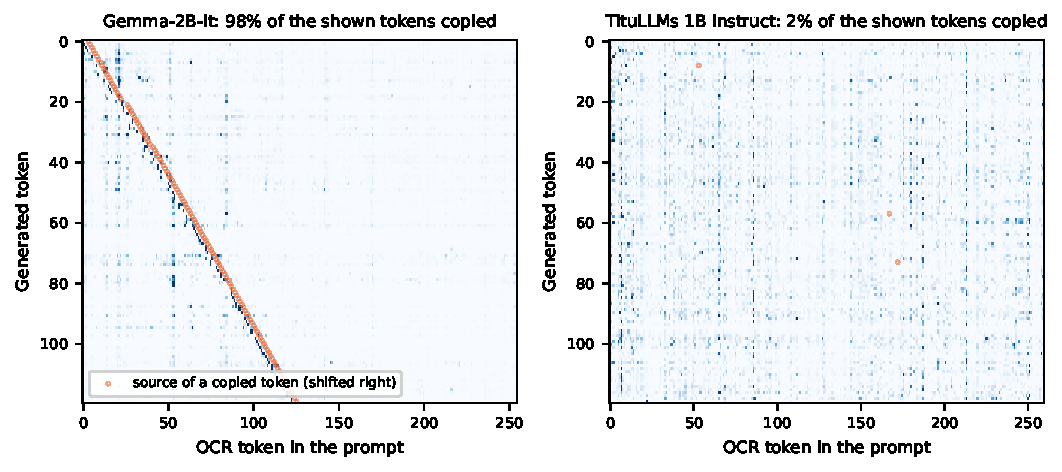
\includegraphics[width=0.85\textwidth]{figures/fig_attribution.pdf}
\caption{Element-wise Grad-CAM maps at mid depth for one chunk of Tesseract text: each row is a generated token, each column an OCR token of the prompt, darker means a larger share of the map (each row scaled to its own maximum). Open circles mark the source of each copied token, drawn three columns to the right so the map stays visible. Left: Gemma-2B-it copies, and the map of each copied token peaks beside its source. Right: TituLLMs 1B Instruct copies almost nothing, and its maps are spread over the prompt.}
\label{fig:attribution}
\end{figure*}

Literal Grad-CAM does not localise: its map peaks on the copied source token for only 0\% to 8\% of copied tokens, close to chance. Averaging the gradient over all positions, as Grad-CAM does for the channels of a CNN, keeps one weight per hidden dimension and discards which position the score depends on; the same weights then highlight every token whose hidden state resembles the source. The element-wise variant keeps the gradient at each position and so avoids this failure.

% ---- begin tables/attribution ----
\begin{table*}[t]
\centering
\caption{Gradient-Based Attribution of Generated Tokens: Token-Level Grad-CAM Maps}
\label{tab:attribution}
\setlength{\tabcolsep}{4pt}
\footnotesize
\begin{tabular}{lcccccccc}
\toprule
 & & \multicolumn{3}{c}{Share of the map (element-wise, mid)} & \multicolumn{4}{c}{Map peaks on the copied source token (\%)} \\
\cmidrule(lr){3-5}\cmidrule(lr){6-9}
Model & \shortstack{Copied\\tokens (\%)} & OCR text & \shortstack{Rest of\\prompt} & \shortstack{Own earlier\\output} & \shortstack{Element-wise\\mid} & \shortstack{Element-wise\\late} & \shortstack{Literal\\mid} & Chance \\
\midrule
\multicolumn{9}{l}{\textit{Tesseract text}} \\
Gemma-2B-it & 99 & 0.47 & 0.09 & 0.44 & 76 & 92 & 3 & 1.2 \\
Qwen3 1.7B & 96 & 0.52 & 0.15 & 0.33 & 73 & 70 & 2 & 1.3 \\
Phi-4-mini & 96 & 0.60 & 0.11 & 0.30 & 81 & 60 & 2 & 1.2 \\
Llama 3.2 1B & 99 & 0.46 & 0.20 & 0.34 & 58 & 68 & 1 & 1.3 \\
BanglaT5 & 11 & 1.00 & -- & -- & 25 & 18 & 2 & 1.5 \\
TituLLMs 1B & 16 & 0.46 & 0.12 & 0.43 & 47 & 43 & 2 & 1.3 \\
TituLLMs 1B Instruct & 21 & 0.28 & 0.16 & 0.55 & 51 & 78 & 4 & 1.5 \\
TituLLMs 3B Instruct & 3 & 0.34 & 0.25 & 0.42 & 20 & 40 & 0 & 1.4 \\
\midrule
\multicolumn{9}{l}{\textit{Clean text}} \\
Gemma-2B-it & 96 & 0.47 & 0.09 & 0.44 & 78 & 89 & 4 & 1.2 \\
Qwen3 1.7B & 96 & 0.51 & 0.15 & 0.35 & 78 & 67 & 1 & 1.3 \\
Phi-4-mini & 90 & 0.55 & 0.09 & 0.36 & 72 & 55 & 2 & 1.2 \\
Llama 3.2 1B & 93 & 0.46 & 0.20 & 0.34 & 65 & 62 & 1 & 1.4 \\
BanglaT5 & 14 & 1.00 & -- & -- & 37 & 43 & 0 & 1.6 \\
TituLLMs 1B & 23 & 0.44 & 0.12 & 0.44 & 41 & 36 & 5 & 1.4 \\
TituLLMs 1B Instruct & 19 & 0.31 & 0.16 & 0.53 & 63 & 56 & 8 & 1.4 \\
TituLLMs 3B Instruct & 25 & 0.50 & 0.17 & 0.33 & 68 & 61 & 6 & 1.4 \\
\bottomrule
\end{tabular}
\par\smallskip
\begin{minipage}{\linewidth}\footnotesize 10 chunks per input (one from each of 10 pages, seed 403), up to 24 generated tokens scored per chunk (240 per model and input; TituLLMs 3B Instruct: 144 on Tesseract and 192 on clean text, because of empty outputs); plain greedy decoding, the main prompt. Score: the logit of each generated token. Literal: Grad-CAM, gradients averaged over positions; element-wise: gradient $\times$ hidden state per position, summed over the hidden dimensions. Mid/late: hidden states at 1/2 and 3/4 of the depth. The first token, special tokens and the predicting position are left out of every map. Copied tokens: output tokens aligned with an identical OCR token. Peak: the largest map value over the OCR text lies within one position of the copied token's source; chance: the rate for a random peak. BanglaT5 is an encoder-decoder model, so its map covers only the encoder input, which is the OCR text.\end{minipage}
\end{table*}
% ---- end tables/attribution ----

\subsection{Page-level safeguards}
\label{sec:safeguards}
The length rule (Table~\ref{tab:safeguards}, appendix) replaces outputs only for three Bengali-pretrained checkpoints, on 5 to 23 of the 40 pages. This lowers their CER, for example from 0.958 to 0.660 for TituLLMs 3B Instruct on Tesseract output, but each remains significantly worse than the raw OCR (there $+0.319$, 95\% CI $[+0.193,+0.460]$, $p=0.001$ after Holm correction over 18 tests); the other models never trigger the rule. The edit-distance cap brings no method significantly below the raw OCR at any $\tau$ (lowest: Qwen3 1.7B on Tesseract output, 0.337 against 0.341, not significant); seven capped results are significantly worse, and for the Bengali-pretrained checkpoints the cap keeps the raw OCR on all but at most two pages.


\subsection{CPU and GPU runs}
\label{sec:cpugpu}
On the five pages whose EasyOCR text was byte-identical between the CPU and the GPU runs, Gemma-2B-it produced the same output on all five, and the outputs of Qwen3 1.7B and Llama 3.2 1B differed from their CPU counterparts by a CER of at most 0.004. The outputs of TituLLMs 1B and BanglaT5 differed more (CER 0.20 and 0.44 between runs), but their scores agreed (0.945 against 0.954 and 0.806 against 0.813). The check is narrow: hardware and precision change together (bfloat16 on the CPU, float32 on the GPU), only five EasyOCR pages qualify, no Tesseract page does because its text changed between the two OCR runs, and the two float16 models were never run on the CPU.

\begin{figure*}[t]
\centering
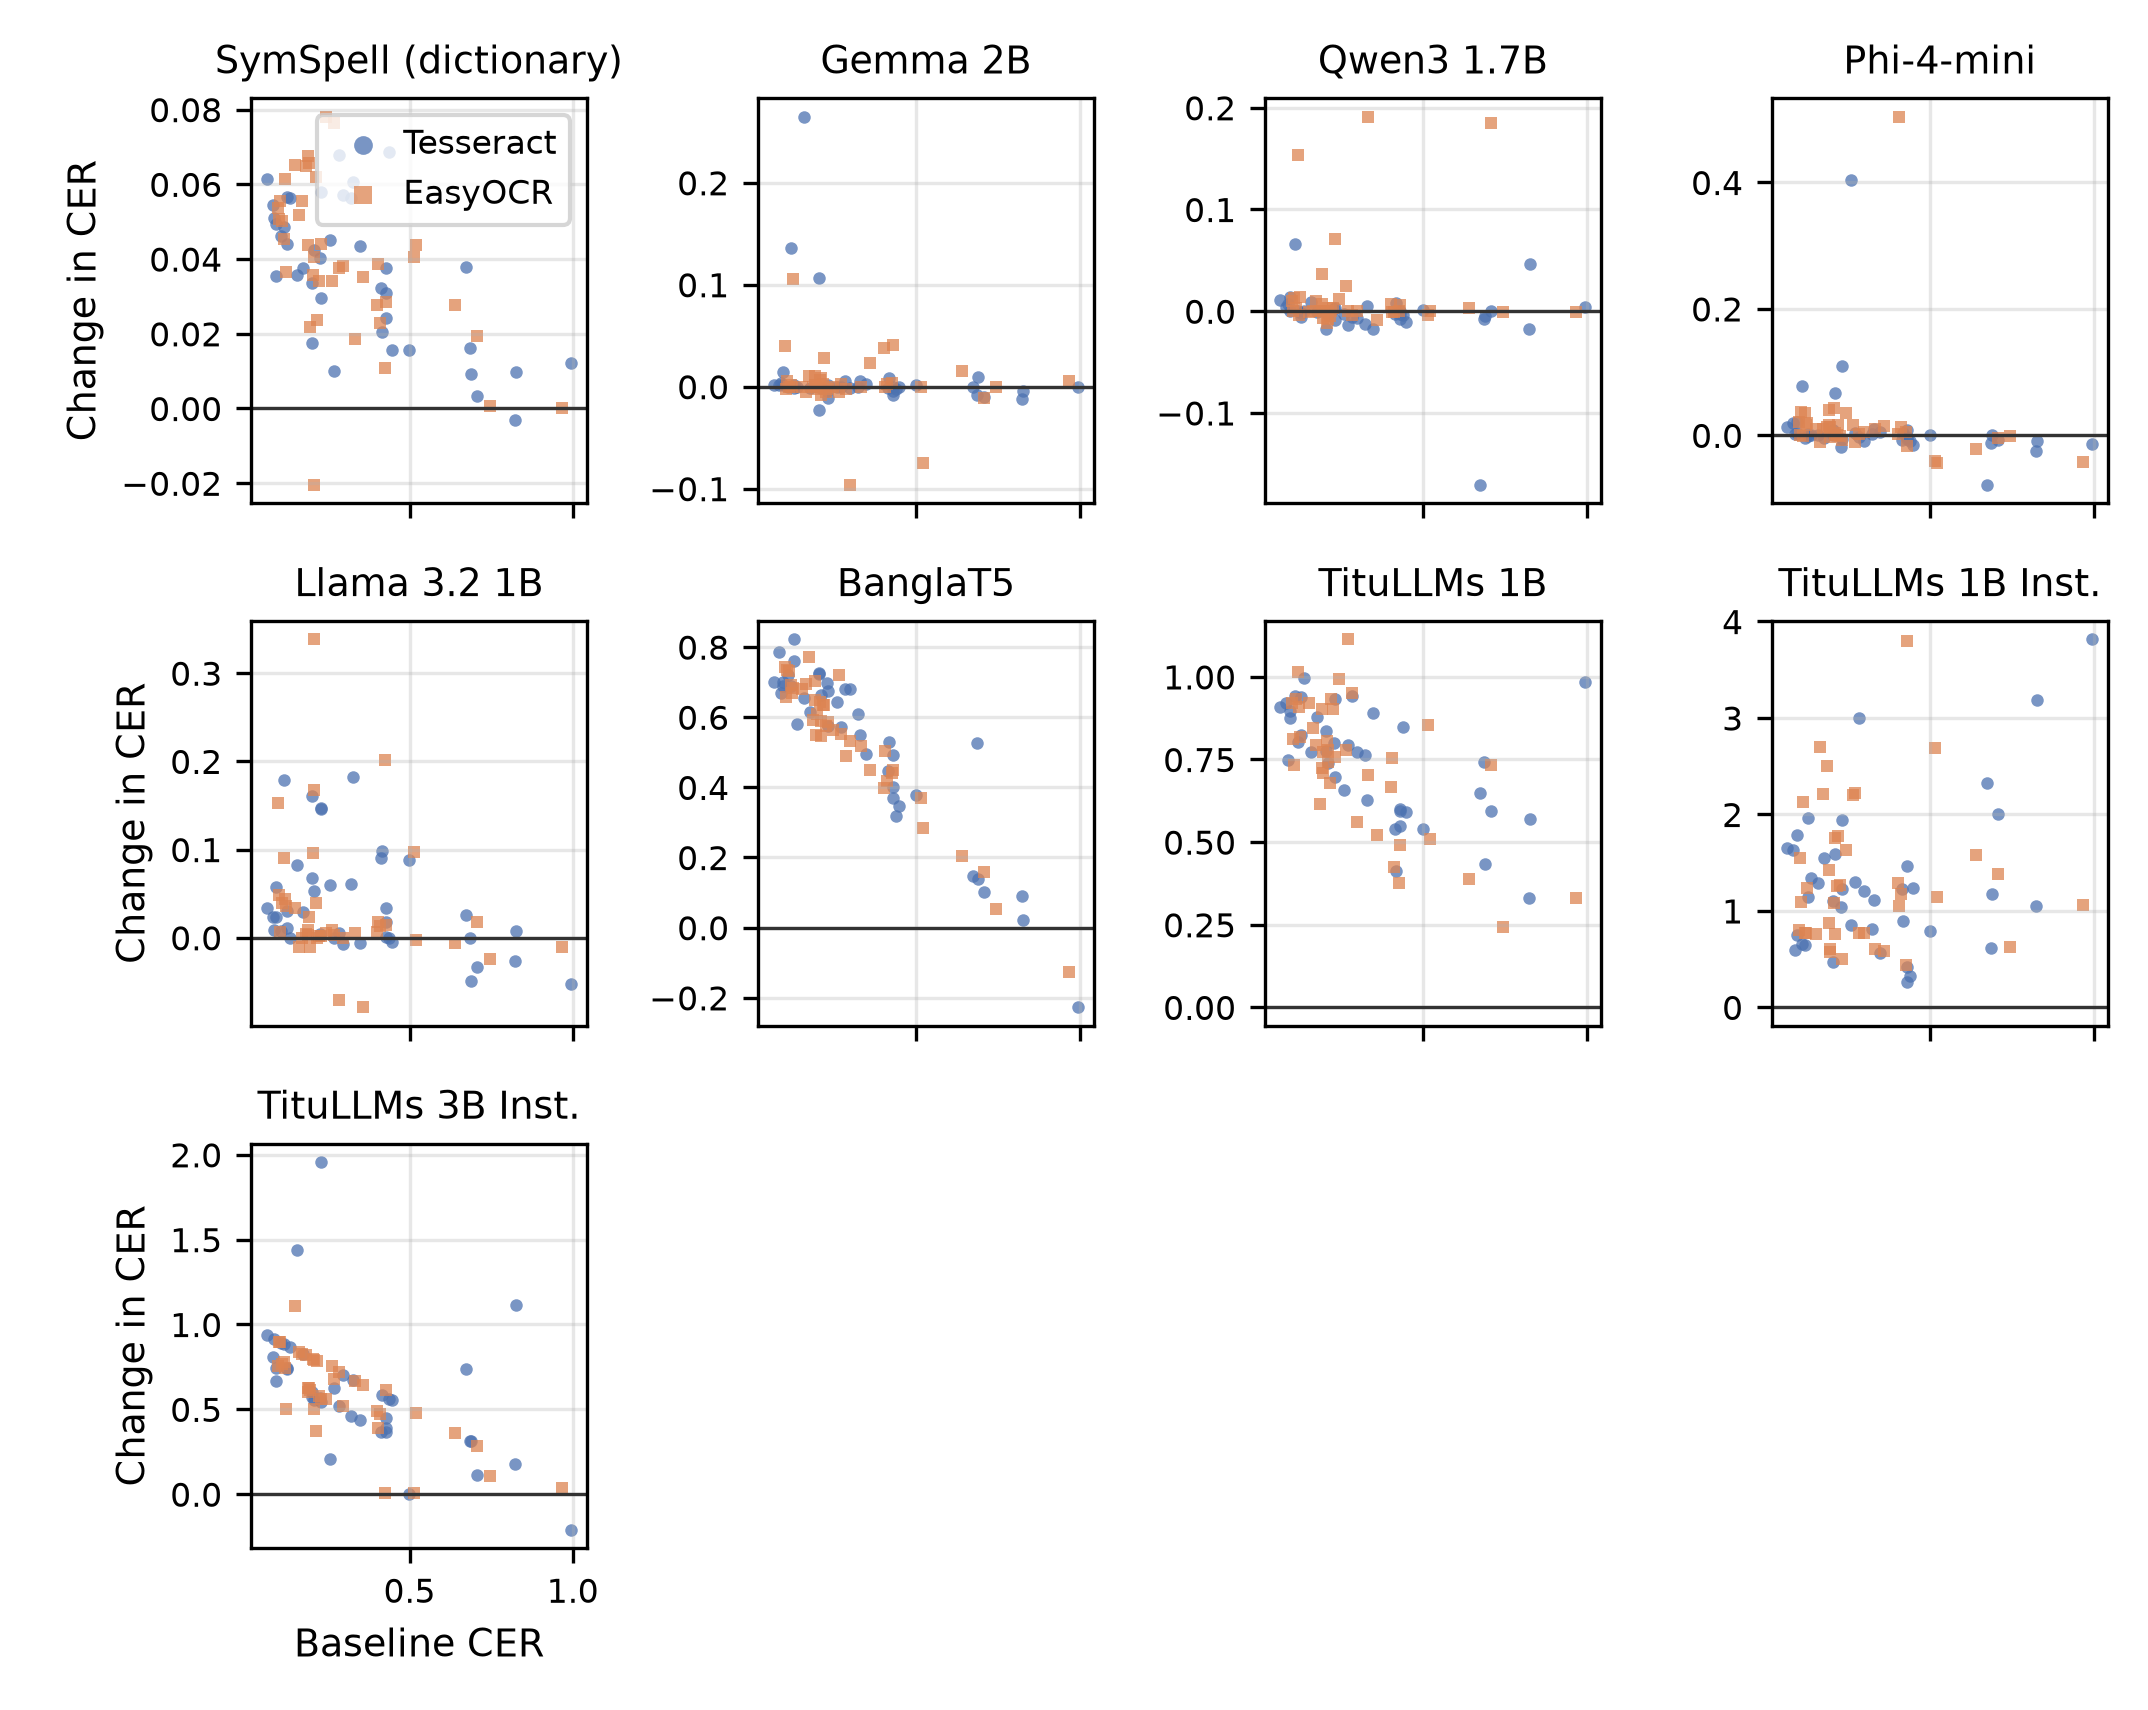
\includegraphics[width=\textwidth]{figures/fig_scatter.png}
\caption{Change in CER per page against the page's baseline CER, one panel per method, for Tesseract (circles) and EasyOCR (squares). Points above the horizontal line are pages the correction made worse. Vertical scales differ between panels.}
\label{fig:scatter}
\end{figure*}

% ---- begin tables/robustness ----
\begin{table*}[t]
\centering
\caption{Robustness of the Main Comparison to the Metric, the Resampling Unit and the Reference}
\label{tab:robustness}
\setlength{\tabcolsep}{4pt}
\footnotesize
\begin{tabular}{lcccccccc}
\toprule
 & & \multicolumn{2}{c}{Grapheme CER} & Books & \multicolumn{2}{c}{Reading order} & \multicolumn{2}{c}{Word recall} \\
\cmidrule(lr){3-4}\cmidrule(lr){5-5}\cmidrule(lr){6-7}\cmidrule(lr){8-9}
Method & \shortstack{Pooled\\CER} & $\Delta$ [95\% CI] & $p_{\mathrm{Holm}}$ & $\Delta$CER 95\% CI & $\Delta$CER & $p_{\mathrm{Holm}}$ & $\Delta$ & $p_{\mathrm{Holm}}$ \\
\midrule
\multicolumn{9}{l}{\textit{Tesseract: raw OCR pooled CER 0.298, grapheme CER 0.431, word recall 0.431 [0.377, 0.488]}} \\
SymSpell (dictionary) & 0.335 & +0.053 [+0.044, +0.061] & $<$0.001 & [+0.031, +0.043] & +0.037 & $<$0.001 & -0.102 & $<$0.001 \\
Gemma-2B-it & 0.315 & +0.010 [-0.002, +0.026] & 1.00\textsuperscript{ns} & [-0.000, +0.027] & +0.012 & 1.00\textsuperscript{ns} & -0.017 & 0.017 \\
Qwen3 1.7B & 0.299 & -0.015 [-0.032, -0.004] & 0.021 & [-0.014, +0.004] & -0.004 & 0.82\textsuperscript{ns} & +0.003 & 0.38\textsuperscript{ns} \\
Phi-4-mini & 0.324 & +0.012 [-0.013, +0.052] & 1.00\textsuperscript{ns} & [-0.003, +0.038] & +0.013 & 1.00\textsuperscript{ns} & -0.028 & $<$0.001 \\
Llama 3.2 1B & 0.343 & +0.028 [+0.009, +0.049] & 0.08\textsuperscript{ns} & [+0.021, +0.058] & +0.038 & 0.002 & -0.034 & $<$0.001 \\
BanglaT5 & 0.857 & +0.462 [+0.350, +0.565] & $<$0.001 & [+0.440, +0.591] & +0.524 & $<$0.001 & -0.386 & $<$0.001 \\
TituLLMs 1B & 1.045 & +0.807 [+0.734, +0.884] & $<$0.001 & [+0.689, +0.795] & +0.748 & $<$0.001 & -0.260 & $<$0.001 \\
TituLLMs 1B Instruct & 1.587 & +1.453 [+1.186, +1.750] & $<$0.001 & [+1.074, +1.545] & +1.306 & $<$0.001 & -0.300 & $<$0.001 \\
TituLLMs 3B Instruct & 0.932 & +0.558 [+0.431, +0.702] & $<$0.001 & [+0.497, +0.763] & +0.623 & $<$0.001 & -0.397 & $<$0.001 \\
\midrule
\multicolumn{9}{l}{\textit{EasyOCR: raw OCR pooled CER 0.286, grapheme CER 0.387, word recall 0.484 [0.444, 0.525]}} \\
SymSpell (dictionary) & 0.325 & +0.054 [+0.044, +0.064] & $<$0.001 & [+0.033, +0.047] & +0.040 & $<$0.001 & -0.113 & $<$0.001 \\
Gemma-2B-it & 0.299 & +0.005 [-0.003, +0.013] & 0.84\textsuperscript{ns} & [-0.006, +0.012] & +0.004 & 0.36\textsuperscript{ns} & -0.019 & 0.002 \\
Qwen3 1.7B & 0.306 & +0.011 [-0.003, +0.030] & 1.00\textsuperscript{ns} & [+0.005, +0.033] & +0.017 & 0.20\textsuperscript{ns} & +0.002 & 0.38\textsuperscript{ns} \\
Phi-4-mini & 0.311 & +0.014 [-0.008, +0.050] & 1.00\textsuperscript{ns} & [+0.000, +0.046] & +0.018 & 0.20\textsuperscript{ns} & -0.026 & $<$0.001 \\
Llama 3.2 1B & 0.322 & +0.021 [+0.001, +0.044] & 0.84\textsuperscript{ns} & [+0.012, +0.055] & +0.031 & 0.012 & -0.027 & $<$0.001 \\
BanglaT5 & 0.832 & +0.468 [+0.393, +0.533] & $<$0.001 & [+0.469, +0.593] & +0.537 & $<$0.001 & -0.454 & $<$0.001 \\
TituLLMs 1B & 1.026 & +0.727 [+0.642, +0.809] & $<$0.001 & [+0.666, +0.800] & +0.737 & $<$0.001 & -0.291 & $<$0.001 \\
TituLLMs 1B Instruct & 1.489 & +1.519 [+1.228, +1.866] & $<$0.001 & [+1.113, +1.575] & +1.338 & $<$0.001 & -0.355 & $<$0.001 \\
TituLLMs 3B Instruct & 0.869 & +0.527 [+0.449, +0.603] & $<$0.001 & [+0.511, +0.665] & +0.592 & $<$0.001 & -0.449 & $<$0.001 \\
\bottomrule
\end{tabular}
\par\smallskip
\begin{minipage}{\linewidth}\footnotesize Pooled CER: total character errors over total reference characters. Grapheme CER: CER over extended grapheme clusters; $\Delta$ = corrected $-$ raw OCR. Books: 95\% interval of the mean change in CER when whole books (37) are resampled instead of pages. Reading order: change in CER against a reference whose regions follow the reading order declared in the PAGE-XML file (17 of 40 references change). Word recall: share of reference word tokens found in the output, ignoring order and extra text; positive $\Delta$ = better; the raw value is followed by its 95\% bootstrap interval. Each $p_{\mathrm{Holm}}$ column is its own exploratory family of 18 tests.\end{minipage}
\end{table*}
% ---- end tables/robustness ----

% ---- begin tables/editops ----
\begin{table}[t]
\centering
\caption{Mean Edit Operations per Page Against the Reference}
\label{tab:editops}
\setlength{\tabcolsep}{4pt}
\footnotesize
\begin{tabular}{llccc}
\toprule
Engine & Model & Subst. & Del. & Ins. \\
\midrule
Tesseract & (no correction) & 92 & 60 & 69 \\
Tesseract & SymSpell (dictionary) & 111 & 71 & 66 \\
Tesseract & Gemma-2B-it & 93 & 76 & 64 \\
Tesseract & Qwen3 1.7B & 92 & 66 & 64 \\
Tesseract & Phi-4-mini & 102 & 70 & 68 \\
Tesseract & Llama 3.2 1B & 90 & 110 & 53 \\
Tesseract & BanglaT5 & 126 & 503 & 5 \\
Tesseract & TituLLMs 1B & 370 & 19 & 384 \\
Tesseract & TituLLMs 1B Instruct & 344 & 33 & 797 \\
Tesseract & TituLLMs 3B Instruct & 170 & 432 & 88 \\
\midrule
EasyOCR & (no correction) & 84 & 58 & 70 \\
EasyOCR & SymSpell (dictionary) & 108 & 68 & 64 \\
EasyOCR & Gemma-2B-it & 83 & 71 & 67 \\
EasyOCR & Qwen3 1.7B & 92 & 62 & 72 \\
EasyOCR & Phi-4-mini & 98 & 68 & 64 \\
EasyOCR & Llama 3.2 1B & 87 & 93 & 59 \\
EasyOCR & BanglaT5 & 181 & 434 & 1 \\
EasyOCR & TituLLMs 1B & 352 & 22 & 385 \\
EasyOCR & TituLLMs 1B Instruct & 350 & 30 & 722 \\
EasyOCR & TituLLMs 3B Instruct & 135 & 458 & 50 \\
\bottomrule
\end{tabular}
\end{table}
% ---- end tables/editops ----

% ---- begin tables/pagetypes ----
\begin{table*}[t]
\centering
\caption{Mean Change in CER by Page Type}
\label{tab:pagetypes}
\setlength{\tabcolsep}{4pt}
\footnotesize
\begin{tabular}{lcccccccc}
\toprule
 & \multicolumn{4}{c}{Tesseract} & \multicolumn{4}{c}{EasyOCR} \\
\cmidrule(lr){2-5}\cmidrule(lr){6-9}
Method & title (10) & verse (8) & prose (13) & list (9) & title (10) & verse (8) & prose (13) & list (9) \\
\midrule
Raw OCR (CER) & 0.319 & 0.334 & 0.199 & 0.576 & 0.255 & 0.293 & 0.184 & 0.511 \\
\midrule
SymSpell (dictionary) & +0.037 & +0.041 & +0.042 & +0.025 & +0.049 & +0.054 & +0.036 & +0.022 \\
Gemma-2B-it & -0.004 & +0.013 & +0.012 & +0.028 & -0.005 & -0.001 & +0.011 & +0.006 \\
Qwen3 1.7B & -0.008 & +0.003 & +0.007 & -0.020 & +0.009 & +0.027 & +0.027 & +0.004 \\
Phi-4-mini & -0.002 & -0.004 & +0.050 & -0.007 & +0.006 & +0.066 & +0.015 & -0.009 \\
Llama 3.2 1B & +0.045 & +0.030 & +0.060 & +0.010 & +0.036 & +0.018 & +0.048 & +0.021 \\
BanglaT5 & +0.567 & +0.546 & +0.650 & +0.252 & +0.576 & +0.544 & +0.629 & +0.340 \\
TituLLMs 1B & +0.797 & +0.723 & +0.774 & +0.654 & +0.740 & +0.839 & +0.814 & +0.524 \\
TituLLMs 1B Instruct & +1.043 & +1.597 & +1.111 & +1.597 & +1.677 & +1.179 & +1.024 & +1.546 \\
TituLLMs 3B Instruct & +0.705 & +0.675 & +0.659 & +0.409 & +0.587 & +0.582 & +0.723 & +0.403 \\
\bottomrule
\end{tabular}
\par\smallskip
\begin{minipage}{\linewidth}\footnotesize First row: mean CER of the raw OCR; other rows: mean change in CER (corrected $-$ raw OCR, positive = worse). Page counts in parentheses. Title: title pages; verse: pages whose main text is metrical, including verse with a commentary; prose: running prose; list: contents, indexes, tables and dictionary entries. Descriptive only: the groups are too small for separate tests.\end{minipage}
\end{table*}
% ---- end tables/pagetypes ----

% ---- begin tables/safeguards ----
\begin{table*}[t]
\centering
\caption{Post-Hoc Safeguards: Length Rule and Edit-Distance Cap (Mean CER, 40 Pages)}
\label{tab:safeguards}
\setlength{\tabcolsep}{4pt}
\footnotesize
\begin{tabular}{lccccccc}
\toprule
 & \multicolumn{3}{c}{Length rule} & \multicolumn{4}{c}{Edit-distance cap $\tau$} \\
\cmidrule(lr){2-4}\cmidrule(lr){5-8}
Method & CER (fallbacks) & $\Delta$CER [95\% CI] & $p_{\mathrm{Holm}}$ & 0.05 & 0.1 & 0.2 & 0.3 \\
\midrule
\multicolumn{8}{l}{\textit{Tesseract: raw OCR CER 0.341}} \\
SymSpell (dictionary) & 0.378 (0/40) & +0.037 [+0.031, +0.043] & $<$0.001 & 0.344 & 0.376$^{+}$ & 0.378$^{+}$ & 0.378$^{+}$ \\
Gemma-2B-it & 0.353 (0/40) & +0.012 [-0.001, +0.029] & 1.00\textsuperscript{ns} & 0.340 & 0.340 & 0.346 & 0.346 \\
Qwen3 1.7B & 0.337 (0/40) & -0.004 [-0.014, +0.005] & 0.70\textsuperscript{ns} & 0.339 & 0.339 & 0.337 & 0.337 \\
Phi-4-mini & 0.354 (0/40) & +0.013 [-0.003, +0.038] & 1.00\textsuperscript{ns} & 0.340 & 0.344 & 0.344 & 0.344 \\
Llama 3.2 1B & 0.380 (0/40) & +0.039 [+0.021, +0.058] & 0.001 & 0.343 & 0.348 & 0.355 & 0.375$^{+}$ \\
BanglaT5 & 0.574 (21/40) & +0.233 [+0.151, +0.317] & 0.001 & 0.341 & 0.341 & 0.341 & 0.341 \\
TituLLMs 1B & 1.084 (0/40) & +0.743 [+0.691, +0.793] & $<$0.001 & 0.341 & 0.341 & 0.341 & 0.341 \\
TituLLMs 1B Instruct & 1.305 (5/40) & +0.964 [+0.785, +1.150] & $<$0.001 & 0.341 & 0.341 & 0.341 & 0.341 \\
TituLLMs 3B Instruct & 0.660 (18/40) & +0.319 [+0.193, +0.460] & 0.001 & 0.341 & 0.341 & 0.341 & 0.341 \\
\midrule
\multicolumn{8}{l}{\textit{EasyOCR: raw OCR CER 0.297}} \\
SymSpell (dictionary) & 0.337 (0/40) & +0.040 [+0.033, +0.046] & $<$0.001 & 0.299 & 0.335$^{+}$ & 0.337$^{+}$ & 0.337$^{+}$ \\
Gemma-2B-it & 0.301 (0/40) & +0.003 [-0.005, +0.012] & 0.48\textsuperscript{ns} & 0.301 & 0.302 & 0.301 & 0.301 \\
Qwen3 1.7B & 0.315 (0/40) & +0.017 [+0.004, +0.033] & 0.18\textsuperscript{ns} & 0.299 & 0.301 & 0.305 & 0.315 \\
Phi-4-mini & 0.315 (0/40) & +0.017 [+0.000, +0.045] & 0.19\textsuperscript{ns} & 0.300 & 0.302 & 0.302 & 0.302 \\
Llama 3.2 1B & 0.330 (0/40) & +0.033 [+0.012, +0.058] & 0.008 & 0.300 & 0.305 & 0.310 & 0.314 \\
BanglaT5 & 0.699 (8/40) & +0.401 [+0.317, +0.483] & $<$0.001 & 0.297 & 0.297 & 0.297 & 0.297 \\
TituLLMs 1B & 1.033 (0/40) & +0.735 [+0.673, +0.794] & $<$0.001 & 0.297 & 0.297 & 0.297 & 0.297 \\
TituLLMs 1B Instruct & 1.231 (6/40) & +0.933 [+0.757, +1.110] & $<$0.001 & 0.297 & 0.297 & 0.297 & 0.297 \\
TituLLMs 3B Instruct & 0.509 (23/40) & +0.212 [+0.124, +0.308] & 0.002 & 0.298 & 0.298 & 0.298 & 0.298 \\
\bottomrule
\end{tabular}
\par\smallskip
\begin{minipage}{\linewidth}\footnotesize Length rule: the raw OCR replaces an output whose length is outside 0.35--2.8 times the input; fallbacks: pages replaced. $\Delta$: safeguarded minus raw OCR (positive = worse); CI: paired bootstrap, 10{,}000 resamples; $p_{\mathrm{Holm}}$: Wilcoxon signed-rank test, Holm-corrected over the 18 length-rule tests. Edit-distance cap: the output is kept only if its CER against the raw OCR is at most $\tau$; $^{+}$/$^{-}$: significantly higher/lower than the raw OCR, Holm-corrected over the 72 cap tests. Both families are exploratory.\end{minipage}
\end{table*}
% ---- end tables/safeguards ----

% Print the appendix tables before the references (editorial review, sec. 5).
\clearpage

% ---- bibliography (compiled from references.bib with IEEEtran.bst) ----
% Generated by IEEEtran.bst, version: 1.14 (2015/08/26)
\begin{thebibliography}{10}
\providecommand{\url}[1]{#1}
\csname url@samestyle\endcsname
\providecommand{\newblock}{\relax}
\providecommand{\bibinfo}[2]{#2}
\providecommand{\BIBentrySTDinterwordspacing}{\spaceskip=0pt\relax}
\providecommand{\BIBentryALTinterwordstretchfactor}{4}
\providecommand{\BIBentryALTinterwordspacing}{\spaceskip=\fontdimen2\font plus
\BIBentryALTinterwordstretchfactor\fontdimen3\font minus
  \fontdimen4\font\relax}
\providecommand{\BIBforeignlanguage}[2]{{%
\expandafter\ifx\csname l@#1\endcsname\relax
\typeout{** WARNING: IEEEtran.bst: No hyphenation pattern has been}%
\typeout{** loaded for the language `#1'. Using the pattern for}%
\typeout{** the default language instead.}%
\else
\language=\csname l@#1\endcsname
\fi
#2}}
\providecommand{\BIBdecl}{\relax}
\BIBdecl

\bibitem{rabby2024enhancement}
\BIBentryALTinterwordspacing
A.~K. M. S.~A. Rabby, H.~Ali, M.~M. Islam, S.~Abujar, and F.~Rahman,
  ``Enhancement of {Bengali} {OCR} by specialized models and advanced
  techniques for diverse document types,'' in \emph{Proceedings of the IEEE/CVF
  Winter Conference on Applications of Computer Vision Workshops (WACVW)},
  2024, pp. 1102--1109. [Online]. Available:
  \url{https://openaccess.thecvf.com/content/WACV2024W/WVLL/papers/Rabby_Enhancement_of_Bengali_OCR_by_Specialized_Models_and_Advanced_Techniques_WACVW_2024_paper.pdf}
\BIBentrySTDinterwordspacing

\bibitem{vershinin2025lightweight}
V.~K. Vershinin, I.~V. Khodnenko, and S.~V. Ivanov, ``Normalization of text
  recognized by optical character recognition using lightweight {LLMs},''
  \emph{Russian Digital Libraries Journal}, vol.~28, no.~5, pp. 1036--1056,
  2025.

\bibitem{thomas2024leveraging}
\BIBentryALTinterwordspacing
A.~Thomas, R.~Gaizauskas, and H.~Lu, ``Leveraging {LLMs} for post-{OCR}
  correction of historical newspapers,'' in \emph{Proceedings of the Third
  Workshop on Language Technologies for Historical and Ancient Languages
  (LT4HALA) @ LREC-COLING-2024}, Torino, Italia, 2024, pp. 116--121. [Online].
  Available: \url{https://aclanthology.org/2024.lt4hala-1.14/}
\BIBentrySTDinterwordspacing

\bibitem{beshirov2025bulgarian}
A.~Beshirov, M.~Dobreva, D.~Dimitrov, M.~Hardalov, I.~Koychev, and P.~Nakov,
  ``Post-{OCR} text correction for {Bulgarian} historical documents,''
  \emph{International Journal on Digital Libraries}, vol.~26, no.~1, p.~4,
  2025.

\bibitem{koynov2025opportunities}
R.~Koynov and T.~H.~A. Doan, ``Opportunities and challenges of {LLMs} as
  post-{OCR} correctors,'' in \emph{Communication Papers of the 20th Conference
  on Computer Science and Intelligence Systems (FedCSIS)}, ser. Annals of
  Computer Science and Information Systems, vol.~45, 2025, pp. 111--118.

\bibitem{kanerva2025nofreelunches}
\BIBentryALTinterwordspacing
J.~Kanerva, C.~Ledins, S.~K{\"a}pyaho, and F.~Ginter, ``{OCR} error
  post-correction with {LLMs} in historical documents: No free lunches,'' in
  \emph{Proceedings of the Third Workshop on Resources and Representations for
  Under-Resourced Languages and Domains (RESOURCEFUL-2025)}, Tallinn, Estonia,
  2025, pp. 38--47. [Online]. Available:
  \url{https://aclanthology.org/2025.resourceful-1.8/}
\BIBentrySTDinterwordspacing

\bibitem{pal2000ocr}
U.~Pal, P.~K. Kundu, and B.~B. Chaudhuri, ``{OCR} error correction of an
  inflectional {Indian} language using morphological parsing,'' \emph{Journal
  of Information Science and Engineering}, vol.~16, no.~6, pp. 903--922, 2000.

\bibitem{ahmed2016improving}
\BIBentryALTinterwordspacing
M.~S. Ahmed, T.~Gon{\c{c}}alves, and H.~Sarwar, ``Improving {Bangla} {OCR}
  output through correction algorithms,'' in \emph{Proceedings of the 10th
  International Conference on Software, Knowledge, Information Management and
  Applications (SKIMA)}.\hskip 1em plus 0.5em minus 0.4em\relax Chengdu, China:
  IEEE, 2016. [Online]. Available: \url{http://hdl.handle.net/10174/20660}
\BIBentrySTDinterwordspacing

\bibitem{joy2026bnmmlu}
S.~S. Joy and S.~Shatabda, ``{BnMMLU}: Measuring massive multitask language
  understanding in {Bengali},'' in \emph{Findings of the Association for
  Computational Linguistics: ACL 2026}.\hskip 1em plus 0.5em minus 0.4em\relax
  San Diego, California, United States: Association for Computational
  Linguistics, 2026, pp. 12\,211--12\,230.

\bibitem{hf2026logits}
\BIBentryALTinterwordspacing
{Hugging Face}, ``Utilities for generation: Logits processors
  ({RepetitionPenaltyLogitsProcessor}, {NoRepeatNGramLogitsProcessor}),''
  Transformers documentation and source,
  \texttt{src/transformers/generation/logits\_process.py}, 2026. [Online].
  Available:
  \url{https://huggingface.co/docs/transformers/internal/generation_utils}
\BIBentrySTDinterwordspacing

\bibitem{safir2021endtoend}
F.~B. Safir, A.~Q. Ohi, M.~F. Mridha, M.~M. Monowar, and M.~A. Hamid,
  ``End-to-end optical character recognition for {Bengali} handwritten words,''
  in \emph{2021 National Computing Colleges Conference (NCCC)}.\hskip 1em plus
  0.5em minus 0.4em\relax IEEE, 2021, pp. 1--7.

\bibitem{chaudhury2022deep}
A.~Chaudhury, P.~S. Mukherjee, S.~Das, C.~Biswas, and U.~Bhattacharya, ``A deep
  {OCR} for degraded {Bangla} documents,'' \emph{ACM Transactions on Asian and
  Low-Resource Language Information Processing}, vol.~21, no.~5, pp. 1--20,
  2022.

\bibitem{nguyen2021survey}
T.~T.~H. Nguyen, A.~Jatowt, M.~Coustaty, and A.~Doucet, ``Survey of post-{OCR}
  processing approaches,'' \emph{ACM Computing Surveys}, vol.~54, no.~6, pp.
  1--37, 2021.

\bibitem{chiron2017icdar}
G.~Chiron, A.~Doucet, M.~Coustaty, and J.-P. Moreux, ``{ICDAR2017} competition
  on post-{OCR} text correction,'' in \emph{Proceedings of the 14th IAPR
  International Conference on Document Analysis and Recognition (ICDAR)}, 2017,
  pp. 1423--1428.

\bibitem{rigaud2019icdar}
C.~Rigaud, A.~Doucet, M.~Coustaty, and J.-P. Moreux, ``{ICDAR} 2019 competition
  on post-{OCR} text correction,'' in \emph{Proceedings of the International
  Conference on Document Analysis and Recognition (ICDAR)}, 2019, pp.
  1588--1593.

\bibitem{rijhwani2020ocr}
S.~Rijhwani, A.~Anastasopoulos, and G.~Neubig, ``{OCR} post correction for
  endangered language texts,'' in \emph{Proceedings of the 2020 Conference on
  Empirical Methods in Natural Language Processing (EMNLP)}, 2020, pp.
  5931--5942.

\bibitem{ehrmann2026hipeocrepair}
M.~Ehrmann, E.~Boros, J.~Opitz, A.~Michail, F.~Wagner, and S.~Clematide,
  ``{ICDAR} 2026 {HIPE-OCRepair} competition on {LLM}-assisted {OCR}
  post-correction for historical documents,'' in \emph{Document Analysis and
  Recognition -- ICDAR 2026}, ser. Lecture Notes in Computer Science.\hskip 1em
  plus 0.5em minus 0.4em\relax Springer, 2026, pp. 405--422.

\bibitem{bourne2025scrambled}
J.~Bourne, ``Scrambled text: Fine-tuning language models for {OCR} error
  correction using synthetic data,'' \emph{International Journal on Document
  Analysis and Recognition (IJDAR)}, vol.~28, no.~4, pp. 741--755, 2025.

\bibitem{boros2024postcorrection}
E.~Boros, M.~Ehrmann, M.~Romanello, S.~Najem-Meyer, and F.~Kaplan,
  ``Post-correction of historical text transcripts with large language models:
  An exploratory study,'' in \emph{Proceedings of the 8th Joint SIGHUM Workshop
  on Computational Linguistics for Cultural Heritage, Social Sciences,
  Humanities and Literature (LaTeCH-CLfL 2024)}.\hskip 1em plus 0.5em minus
  0.4em\relax St. Julians, Malta: Association for Computational Linguistics,
  2024, pp. 133--159.

\bibitem{danilova2025german}
\BIBentryALTinterwordspacing
V.~Danilova and G.~Aangenendt, ``Post-{OCR} correction of historical {German}
  periodicals using {LLMs},'' in \emph{Proceedings of the Third Workshop on
  Resources and Representations for Under-Resourced Languages and Domains
  (RESOURCEFUL-2025)}, Tallinn, Estonia, 2025, pp. 120--129. [Online].
  Available: \url{https://aclanthology.org/2025.resourceful-1.26/}
\BIBentrySTDinterwordspacing

\bibitem{viana2026reframing}
C.~M. Viana, ``Reframing historical text extraction: A cross-pathway validation
  of {OCR}, {LLM}-assisted correction, and direct multimodal transcription,''
  \emph{Information}, vol.~17, no.~8, p. 722, 2026.

\bibitem{zhang2024prosody}
J.~Zhang, W.~Haverals, M.~Naydan, and B.~W. Kernighan, ``Post-{OCR} correction
  with {OpenAI}'s {GPT} models on challenging {English} prosody texts,'' in
  \emph{Proceedings of the ACM Symposium on Document Engineering (DocEng
  '24)}.\hskip 1em plus 0.5em minus 0.4em\relax San Jose, CA, USA: Association
  for Computing Machinery, 2024.

\bibitem{do2025reference}
T.~Do, D.~P. Tran, A.~Vo, and D.~Kim, ``Reference-based post-{OCR} processing
  with {LLM} for precise diacritic text in historical document recognition,''
  in \emph{Proceedings of the AAAI Conference on Artificial Intelligence},
  vol.~39, no.~27, 2025, pp. 27\,951--27\,959.

\bibitem{levchenko2025historical}
\BIBentryALTinterwordspacing
M.~A. Levchenko, ``Evaluating {LLMs} for historical document {OCR}: A
  methodological framework for digital humanities,'' in \emph{Proceedings of
  the First Workshop on Natural Language Processing and Language Models for
  Digital Humanities (LM4DH 2025)}, Varna, Bulgaria, 2025, pp. 75--85.
  [Online]. Available: \url{https://aclanthology.org/2025.lm4dh-1.7/}
\BIBentrySTDinterwordspacing

\bibitem{bhattacharjee2022banglabert}
A.~Bhattacharjee, T.~Hasan, W.~Ahmad, K.~S. Mubasshir, M.~S. Islam, A.~Iqbal,
  M.~S. Rahman, and R.~Shahriyar, ``{BanglaBERT}: Language model pretraining
  and benchmarks for low-resource language understanding evaluation in
  {Bangla},'' in \emph{Findings of the Association for Computational
  Linguistics: NAACL 2022}, Seattle, USA, 2022, pp. 1318--1327.

\bibitem{bhattacharjee2023banglat5}
A.~Bhattacharjee, T.~Hasan, W.~U. Ahmad, and R.~Shahriyar, ``{BanglaNLG} and
  {BanglaT5}: Benchmarks and resources for evaluating low-resource natural
  language generation in {Bangla},'' in \emph{Findings of the Association for
  Computational Linguistics: EACL 2023}, 2023, checkpoint: csebuetnlp/banglat5.

\bibitem{nahin2025titullms}
\BIBentryALTinterwordspacing
S.~K. Nahin, R.~N. Nandi, S.~Sarker, Q.~S. Muhtaseem, M.~Kowsher, A.~C. Shill,
  M.~Ibrahim, M.~H. Menon, T.~A. Muntasir, and F.~Alam, ``{TituLLMs}: A family
  of {Bangla} {LLMs} with comprehensive benchmarking,'' in \emph{Findings of
  the Association for Computational Linguistics: ACL 2025}, Vienna, Austria,
  2025, pp. 24\,922--24\,940. [Online]. Available:
  \url{https://aclanthology.org/2025.findings-acl.1279/}
\BIBentrySTDinterwordspacing

\bibitem{zehady2026banglallama}
\BIBentryALTinterwordspacing
A.~K. Zehady, S.~R. Dipta, N.~Islam, S.~A. Mamun, and S.~Karmaker,
  ``{BanglaLlama}: {LLaMA} for {Bangla} language,'' in \emph{Proceedings of the
  Second Workshop on Language Models for Low-Resource Languages (LoResLM
  2026)}, 2026, pp. 73--89. [Online]. Available:
  \url{https://aclanthology.org/2026.loreslm-1.7/}
\BIBentrySTDinterwordspacing

\bibitem{mahfuz2025toolate}
\BIBentryALTinterwordspacing
T.~Mahfuz, S.~K. Dey, R.~Naswan, H.~Adil, K.~S. Sayeed, and H.~S. Shahgir,
  ``Too late to train, too early to use? a study on necessity and viability of
  low-resource {Bengali} {LLMs},'' in \emph{Proceedings of the 31st
  International Conference on Computational Linguistics (COLING 2025)}, Abu
  Dhabi, UAE, 2025, pp. 1183--1200. [Online]. Available:
  \url{https://aclanthology.org/2025.coling-main.79/}
\BIBentrySTDinterwordspacing

\bibitem{petrov2023tokenizer}
\BIBentryALTinterwordspacing
A.~Petrov, E.~L. Malfa, P.~H.~S. Torr, and A.~Bibi, ``Language model tokenizers
  introduce unfairness between languages,'' in \emph{Advances in Neural
  Information Processing Systems 36 (NeurIPS 2023)}, 2023. [Online]. Available:
  \url{https://proceedings.neurips.cc/paper_files/paper/2023/hash/74bb24dca8334adce292883b4b651eda-Abstract-Conference.html}
\BIBentrySTDinterwordspacing

\bibitem{ahia2023cost}
\BIBentryALTinterwordspacing
O.~Ahia, S.~Kumar, H.~Gonen, J.~Kasai, D.~Mortensen, N.~Smith, and Y.~Tsvetkov,
  ``Do all languages cost the same? tokenization in the era of commercial
  language models,'' in \emph{Proceedings of the 2023 Conference on Empirical
  Methods in Natural Language Processing}, 2023, pp. 9904--9923. [Online].
  Available: \url{https://aclanthology.org/2023.emnlp-main.614/}
\BIBentrySTDinterwordspacing

\bibitem{bhattacharyya2025banglagec}
\BIBentryALTinterwordspacing
P.~Bhattacharyya and A.~Bhattacharya, ``Leveraging {LLMs} for {Bangla} grammar
  error correction: Error categorization, synthetic data, and model
  evaluation,'' in \emph{Findings of the Association for Computational
  Linguistics: ACL 2025}, 2025, pp. 8220--8239. [Online]. Available:
  \url{https://aclanthology.org/2025.findings-acl.431/}
\BIBentrySTDinterwordspacing

\bibitem{kumar2026postasr}
\BIBentryALTinterwordspacing
R.~Kumar, A.~Krishna, G.~Ramakrishnan, and P.~Jyothi, ``Post-{ASR} correction
  in {Hindi}: Comparing language models and large language models in
  low-resource scenarios,'' in \emph{Proceedings of the 19th Conference of the
  European Chapter of the Association for Computational Linguistics (Volume 2:
  Short Papers)}, 2026, pp. 636--645. [Online]. Available:
  \url{https://aclanthology.org/2026.eacl-short.45/}
\BIBentrySTDinterwordspacing

\bibitem{maheshwari2022sanskrit}
A.~Maheshwari, N.~Singh, A.~Krishna, and G.~Ramakrishnan, ``A benchmark and
  dataset for post-{OCR} text correction in {Sanskrit},'' in \emph{Findings of
  the Association for Computational Linguistics: EMNLP 2022}.\hskip 1em plus
  0.5em minus 0.4em\relax Association for Computational Linguistics, 2022, pp.
  6258--6265.

\bibitem{bhandari2026contextual}
A.~Bhandari and G.~Harit, ``A framework and dataset for contextual post-{OCR}
  correction,'' \emph{ACM Transactions on Asian and Low-Resource Language
  Information Processing}, vol.~25, no.~6, 2026.

\bibitem{rahman2023bspell}
C.~R. Rahman, M.~H. Rahman, S.~Zakir, M.~Rafsan, and M.~E. Ali, ``{BSpell}: A
  {CNN}-blended {BERT} based {Bangla} spell checker,'' in \emph{Proceedings of
  the First Workshop on Bangla Language Processing (BLP-2023)}, Singapore,
  2023, pp. 7--17.

\bibitem{bijoy2025transformer}
M.~H. Bijoy, N.~Hossain, S.~Islam, and S.~Shatabda, ``A transformer-based
  spelling error correction framework for {Bangla} and resource scarce {Indic}
  languages,'' \emph{Computer Speech \& Language}, vol.~89, p. 101703, 2025.

\bibitem{clausner2019reid}
C.~Clausner, A.~Antonacopoulos, T.~Derrick, and S.~Pletschacher, ``{ICDAR2019}
  competition on recognition of early {Indian} printed documents
  ({REID2019}),'' in \emph{Proceedings of the 15th International Conference on
  Document Analysis and Recognition (ICDAR)}, Sydney, Australia, 2019.

\bibitem{britishlibrary2019bengaligt}
\BIBentryALTinterwordspacing
T.~Derrick and {British Library}, ``Ground truth transcriptions for training
  {OCR} of historical {Bengali} printed texts -- {Recognition} of early
  {Indian} printed documents competition -- updated with improved {XML}
  coordinates,'' Dataset, version 2. British Library Research Repository. 81
  images (400 dpi TIFF) with PAGE XML transcriptions, books printed 1713--1914;
  Public Domain Mark 1.0, 2020. [Online]. Available:
  \url{https://bl.iro.bl.uk/concern/datasets/bb125e50-4a09-46e8-904b-6e46cf308d91}
\BIBentrySTDinterwordspacing

\bibitem{smith2007tesseract}
R.~Smith, ``An overview of the {Tesseract} {OCR} engine,'' in \emph{Proceedings
  of the 9th International Conference on Document Analysis and Recognition
  (ICDAR)}, Curitiba, Brazil, 2007, pp. 629--633.

\bibitem{tesseract5}
{Tesseract OCR contributors}, ``Tesseract open source {OCR} engine, version
  5,'' \url{https://github.com/tesseract-ocr/tesseract}. Version 5.3.4 used,
  2021.

\bibitem{jaidedai2024easyocr}
\BIBentryALTinterwordspacing
{JaidedAI}, ``{EasyOCR}: Ready-to-use {OCR} with 80+ supported languages,''
  Software, version 1.7.2, 2024. [Online]. Available:
  \url{https://github.com/JaidedAI/EasyOCR}
\BIBentrySTDinterwordspacing

\bibitem{wolf2020transformers}
T.~Wolf \emph{et~al.}, ``Transformers: State-of-the-art natural language
  processing,'' in \emph{Proceedings of the 2020 Conference on Empirical
  Methods in Natural Language Processing: System Demonstrations}, 2020, pp.
  38--45.

\bibitem{wiher2022decoding}
G.~Wiher, C.~Meister, and R.~Cotterell, ``On decoding strategies for neural
  text generators,'' \emph{Transactions of the Association for Computational
  Linguistics}, vol.~10, pp. 997--1012, 2022.

\bibitem{gemma2024card}
{Google}, ``{gemma-2b-it} (gemma 1) model card,'' Hugging Face model card:
  \url{https://huggingface.co/google/gemma-2b-it}, revision 9698841, 2024.

\bibitem{qwen2025card}
{Qwen Team}, ``{Qwen3} model cards ({Qwen3-0.6B}, {1.7B}, {4B}, {8B}, {32B}),''
  Hugging Face model cards, e.g.\ \url{https://huggingface.co/Qwen/Qwen3-1.7B},
  revision 70d244c, 2025.

\bibitem{phi4mini2025card}
{Microsoft}, ``{Phi-4-mini-instruct} model card,'' Hugging Face model card:
  \url{https://huggingface.co/microsoft/Phi-4-mini-instruct}, revision cfbefac,
  2025.

\bibitem{meta2024llama32}
{Meta AI}, ``Llama 3.2: Multilingual large language models,'' Model card:
  \url{https://huggingface.co/meta-llama/Llama-3.2-1B-Instruct}, revision
  9213176, 2024.

\bibitem{garbe2025symspell}
W.~Garbe, ``{SymSpell}: Symmetric delete spelling correction algorithm,''
  \url{https://github.com/wolfgarbe/SymSpell}. Python port symspellpy 6.10.0
  used, 2025.

\bibitem{dave2018frequencywords}
H.~Dave, ``{FrequencyWords}: Frequency word lists generated from
  {OpenSubtitles2018},'' \url{https://github.com/hermitdave/FrequencyWords}.
  Bengali list bn\_50k, CC BY-SA 4.0, 2018.

\bibitem{wikimedia2023wikipedia}
\BIBentryALTinterwordspacing
{Wikimedia Foundation}, ``{Wikipedia} dataset, {Bengali} dump of 1 {November}
  2023 (\texttt{wikimedia/wikipedia}, configuration \texttt{20231101.bn}),''
  Hugging Face dataset, 2023. [Online]. Available:
  \url{https://huggingface.co/datasets/wikimedia/wikipedia}
\BIBentrySTDinterwordspacing

\bibitem{vaessen2022jiwer}
\BIBentryALTinterwordspacing
N.~Vaessen, ``{JiWER}: Similarity measures for automatic speech recognition
  evaluation,'' Software, version 4.0.0, 2022. [Online]. Available:
  \url{https://github.com/jitsi/jiwer}
\BIBentrySTDinterwordspacing

\bibitem{wilcoxon1945}
F.~Wilcoxon, ``Individual comparisons by ranking methods,'' \emph{Biometrics
  Bulletin}, vol.~1, no.~6, pp. 80--83, 1945.

\bibitem{holm1979}
S.~Holm, ``A simple sequentially rejective multiple test procedure,''
  \emph{Scandinavian Journal of Statistics}, vol.~6, no.~2, pp. 65--70, 1979.

\bibitem{selvaraju2017gradcam}
R.~R. Selvaraju, M.~Cogswell, A.~Das, R.~Vedantam, D.~Parikh, and D.~Batra,
  ``{Grad-CAM}: Visual explanations from deep networks via gradient-based
  localization,'' in \emph{Proceedings of the IEEE International Conference on
  Computer Vision (ICCV)}, 2017, pp. 618--626.

\bibitem{gemma3card2025}
{Google}, ``{Gemma 3} model cards ({gemma-3-1b-it}, {gemma-3-4b-it}),'' Hugging
  Face model cards: \url{https://huggingface.co/google/gemma-3-1b-it},
  \url{https://huggingface.co/google/gemma-3-4b-it}, 2025.

\bibitem{dettmers2023qlora}
T.~Dettmers, A.~Pagnoni, A.~Holtzman, and L.~Zettlemoyer, ``{QLoRA}: Efficient
  finetuning of quantized {LLMs},'' in \emph{Advances in Neural Information
  Processing Systems (NeurIPS)}, 2023.

\bibitem{xue2022byt5}
L.~Xue, A.~Barua, N.~Constant, R.~Al-Rfou, S.~Narang, M.~Kale, A.~Roberts, and
  C.~Raffel, ``{ByT5}: Towards a token-free future with pre-trained
  byte-to-byte models,'' \emph{Transactions of the Association for
  Computational Linguistics}, vol.~10, pp. 291--306, 2022.

\bibitem{rahman2026repo}
\BIBentryALTinterwordspacing
A.~Rahman, ``bengali-postocr-sllm: Code, data splits and evaluation for
  zero-shot post-{OCR} correction of {Bengali},'' GitHub repository, 2026.
  [Online]. Available:
  \url{https://github.com/Ariffurrhmn/bengali-postocr-sllm}
\BIBentrySTDinterwordspacing

\end{thebibliography}

\end{document}
